\documentclass[10pt]{book}
\usepackage[utf8]{inputenc}
\usepackage[a4paper]{geometry}
\usepackage{fix-cm}
\usepackage{chngpage}
\usepackage{graphicx}
\usepackage{color}
\usepackage{makeidx}
\usepackage{longtable}
\usepackage{colortbl}
\usepackage[table]{xcolor}
\usepackage{underscore}
\usepackage{caption}
\usepackage{amsmath}
\usepackage{float}
\usepackage{array}
\usepackage{datatool}
\usepackage{subfigure}
\usepackage{fancyhdr}
\usepackage[Bjarne]{fncychap}
\usepackage{listings}
\usepackage{bold-extra}
\usepackage{lettrine}
\usepackage{booktabs}
\usepackage{multirow}
\definecolor{seagreen}{RGB}{64,100,120}
\definecolor{darkpink}{RGB}{200,100,120}
\definecolor{light-gray}{gray}{0.85}
\definecolor{medium-gray}{gray}{0.5}
\usepackage[colorlinks=true,linkcolor=seagreen,citecolor=darkpink]{hyperref}
\usepackage{path}
\usepackage{tikz}
\usetikzlibrary{arrows,positioning,automata,shadows,shapes,snakes,patterns,decorations,calc}
\usetikzlibrary{arrows,arrows.meta,positioning,automata,shadows,shapes,shapes.callouts,snakes,patterns,decorations,calc,shadows.blur}
\usepackage{adjustbox}
\usepackage[most]{tcolorbox}


%
% custom options
%
\renewcommand{\captionlabelfont}{\small \bf}
\renewcommand{\captionfont}{\small \it}
\setlength{\parindent}{0mm}
\setlength{\parskip}{.5\baselineskip}
\fancyhead{} % clear all header fields
\fancyhead[RO,LE]{\thepage}
\fancyhead[LO,RE]{\nouppercase{\rightmark}}
\fancyfoot{} % clear all footer fields
%\fancyfoot[LO,RE]{\slshape The Trampoline Handbook}
\fancyfoot[RO,LE]{\slshape\nouppercase{\leftmark}}
\renewcommand{\headrulewidth}{0.4pt}
\renewcommand{\footrulewidth}{0.4pt}
\pagestyle{fancy}
\ChTitleVar{\raggedleft\Huge\sffamily}
\ChNameVar{\raggedleft\normalsize\sffamily}
\ChNumVar{\raggedleft\bfseries\Large\sffamily}

%
% C language options
%
\lstset{
  language=C,
  basicstyle=\ttfamily\footnotesize,
  commentstyle=\itshape\color{cyan}
}

%
% OIL language options
%
\lstdefinelanguage{OIL}
{
  morekeywords= {
  	  APPMODE,
	  BUILD,
	  STATUS,
	  APP_SRC, 
	  TRAMPOLINE_BASE_PATH,
	  LDFLAGS,
	  APP_NAME,
	  OIL_VERSION,
	  SYSTEM,
	  TRUE,
	  EXTENDED,
	  AUTOSTART,
	  ACTIVATION,
	  IMPLEMENTATION,
	  RESOURCE, RESOURCEPROPERTY, STANDARD, INTERNAL, LINKED, LINKEDRESOURCE,
	  TASK, SCHEDULE, FULL, NONE, PRIORITY, EVENT, ISR, CATEGORY, OS, CPU, MEMMAP,
	  COMPILER, LINKER, SCRIPT, IOC, DATATYPENAME, DATATYPEPROPERTY, RECEIVER, SENDER, RCV_OSAPPLICATION, 	  RECEIVER_PULL_CB, ACTION, SENDER_ID, SND_OSAPPLICATION, FALSE, GDBCOMMANDS, PORT
	}
}

\lstset{
  language=OIL,
%  emph={
%    var,
%    expression,
%    string,
%    instruction_list,
%    template_file_name,
%    reader,
%    hierarchy
%  },
  emphstyle=\em,
  moredelim=[s]{"}{"},
  basicstyle=\ttfamily\small}

\lstdefinelanguage{goilTemplate}
{
  morekeywords= {
	  after,
	  before,
	  between,
	  block,
	  default,
	  do,
	  else,
	  elsif,
	  emptylist,
	  end,
	  error,
	  exists,
	  false,
	  for,
	  foreach,
	  from,
	  here,
	  let,
	  loop,
	  no,
	  if,
	  in,
	  mod,
	  not,
	  or,
	  prefixedby,
	  template,
	  then,
	  to,
	  true,
	  yes,
	  warning,
	  while,
	  write,
	  !,
	  ?
	}
}

\lstset{
  language=goilTemplate,
  emph={
    var,
    expression,
    string,
    instruction_list,
    template_file_name,
    reader,
    hierarchy
  },
  emphstyle=\em,
  moredelim=[s][\color{blue}]{\%}{\%},
  moredelim=[s]{"}{"},
  morecomment=[l][\color{medium-gray}\itshape]{\#},
  basicstyle=\ttfamily\small,
  morekeywords=\bfseries
}

% Inline color boxes

\newtcbox{\inlinebox}[1][red]{
	on line,
	arc=0pt,
	outer arc=0pt,
	colback=#1!10!white,
	colframe=#1!50!black,
	boxsep=0pt,
	left=2pt,
	right=2pt,
	top=1pt,
	bottom=1pt,
	boxrule=.25pt
}

%
% Commands for paragraph types
%
%\newcommand{\note}[1]{\vspace{1mm}\fbox{\begin{minipage}[t]{.1\linewidth}{\bfseries Note:}\end{minipage}%
%\hfill\begin{minipage}[t]{.885\linewidth}#1\end{minipage}}\vspace{1mm}}
\newcommand{\note}[1]{%
\hspace{-12.4mm}
\rowcolors{1}{white}{white}
\begin{tabular}[b]{m{5mm}|m{\linewidth}}

\includegraphics[width=6mm,angle=45]{pictures/note} & #1\\
\end{tabular}
}
\newcommand{\warning}[1]{%
\hspace{-14.2mm}
\rowcolors{1}{white}{light-gray}
\begin{tabular}[b]{m{7mm}|m{\linewidth}}
\includegraphics[width=7mm]{pictures/warn} & #1\\
\end{tabular}
}
%
% Commands for inline formatting of C computing language
%
\newcommand{\argu}[1]{{\ttfamily #1}}
\newcommand{\ctype}[1]{{\small\ttfamily #1}}
\newcommand{\cdata}[1]{{\ttfamily #1}}
\newcommand{\var}[1]{{\ttfamily\em #1}}
\newcommand{\va}{\small\ttfamily\em}
\newcommand{\cfunction}[1]{{\ttfamily #1}}
\newcommand{\pyfunction}[1]{{\ttfamily #1}}
\newcommand{\cmacro}[1]{{\small\ttfamily #1}}
\newcommand{\constant}[1]{{\small\ttfamily #1}}
\newcommand{\oilobj}[1]{\lstinline[language=OIL]{#1}}
\newcommand{\oilattr}[1]{\lstinline[language=OIL]{#1}}
\newcommand{\oilattren}[1]{\texttt{#1}}
\newcommand{\oilval}[1]{\lstinline[language=OIL]{#1}}
\newcommand{\member}[1]{{\small\ttfamily #1}}
\newcommand{\mem}{\small\ttfamily}

%
% Commands for other formatting
%
\newcommand{\tool}[1]{{\small\ttfamily #1}}
\newcommand{\toolarg}[1]{{\small\ttfamily #1}}
\newcommand{\com}[1]{\inlinebox[blue]{\small\ttfamily #1}}
\newcommand{\comoutput}[1]{{\small\ttfamily #1}}
\newcommand{\file}[1]{{\small\ttfamily `#1'}}
\newcommand{\envvar}[1]{{\scriptsize\sffamily #1}}
\newcommand{\longprogramopt}[1]{{\small\ttfamily --#1}}
\newcommand{\programopt}[1]{{\ttfamily -#1}}
\newcommand{\strong}[1]{{\bf #1}}
\newcommand{\ie}{i.e.}
\newcommand{\asfct}[1]{\texttt{#1}}
\newcommand{\hex}[1]{\texttt{#1$_H$}}
\newcommand{\reg}[1]{\textit{#1}}
\newcommand{\dreg}[1]{{\small\ttfamily #1}}
\newcommand{\idxconfflag}[1]{{\footnotesize\ttfamily #1}\index{Configuration macros!#1}\index{#1}}
\newcommand{\toreplace}[1]{{\footnotesize $<$}#1{\footnotesize $>$}}
%\newcommand{\figcaption}[2]{\textit{\caption{\small #1}}\label{#2}}
\newcommand{\goil}{\tool{goil}\index{goil, The OIL/arXML compiler of Trampoline}}
\newcommand{\process}{process\index{process, a task, basic or extended, or an ISR category 2}}
\newcommand{\sysgen}{system generation tool\index{system generation tool, the tool that takes as an input a description of the system (in OIL or in XML) to generate the corresponding .c and .h files.}}
\newcommand{\stringlit}[1]{{\small\ttfamily "{#1}"}}
\newcommand{\character}[1]{{\small\ttfamily `{#1}'}}
\newcommand{\api}[1]{\cfunction{#1}\index{#1}}
\newcommand{\osek}{OSEK}
\newcommand{\autosar}{{\small AUTOSAR}}
\newcommand{\posix}{POSIX}
\newenvironment{penum}{
\begin{enumerate}
  \setlength{\itemsep}{1pt}
  \setlength{\parskip}{0pt}
  \setlength{\parsep}{0pt}
}{\end{enumerate}}
\newenvironment{pitemize}{
\begin{itemize}
  \setlength{\itemsep}{1pt}
  \setlength{\parskip}{0pt}
  \setlength{\parsep}{0pt}
}{\end{itemize}}

%
% Graphic symbols for scheduling diagrams
%
\newcommand{\activate}{\includegraphics[height=9pt]{pictures/activate.pdf}}
\newcommand{\terminate}{\includegraphics[height=9pt]{pictures/terminate.pdf}}

%
% states of a task
%
\newcommand{\RUNNING}{\constant{RUNNING}\index{RUNNING, state of a task}}
\newcommand{\READY}{\constant{READY}\index{READY, state of a task}}
\newcommand{\SUSPENDED}{\constant{SUSPENDED}\index{SUSPENDED, state of a task}}
\newcommand{\WAITING}{\constant{WAITING}\index{WAITING, state of a task}}
\newcommand{\AUTOSTART}{\constant{AUTOSTART}\index{AUTOSTART, state of a task}}
\newcommand{\READYANDNEW}{\constant{READY\_AND\_NEW}\index{READY_AND_NEW, state of a task}}

%
% Kind of task
%
\newcommand{\BASIC}{\constant{BASIC}\index{BASIC, compilation with no extended error checking}}
\newcommand{\EXTENDED}{\constant{EXTENDED}\index{EXTENDED, compilation with extended error checking}}

%
% result codes
%
\newcommand{\OK}{E\_OK}
\newcommand{\OSID}{E\_OS\_ID}
\newcommand{\OSLIMIT}{E\_OS\_LIMIT}
\newcommand{\OSRESOURCE}{E\_OS\_RESOURCE}
\newcommand{\OSCALLLEVEL}{E\_OS\_CALLEVEL}
\newcommand{\OSPROTECTIONMEMORY}{E\_OS\_PROTECTION\_MEMORY}
\newcommand{\OSACCESS}{E\_OS\_ACCESS}
\newcommand{\OSSTATE}{E\_OS\_STATE}

%
% Scalability class
%
\newcommand{\SC}[1]{scalability class #1}

%
% OIL attribute
%
\newcommand{\PRIORITY}{PRIORITY\index{PRIORITY}}
\newcommand{\SCHEDULE}{SCHEDULE\index{SCHEDULE}}
\newcommand{\TRUE}{{\small\ttfamily TRUE}}
\newcommand{\FALSE}{{\small\ttfamily FALSE}}

%
% Conf macros
%
\newcommand{\YES}{{\small\ttfamily YES}}
\newcommand{\NO}{{\small\ttfamily NO}}

%
% environment and commands to describe system services
%
\newcommand{\servicename}{}
\newcommand{\apiname}{}
\newcommand{\servicedescription}{}
\newcommand{\servicereturn}{}
\DTLnewdb{argDB}
\DTLnewdb{resDB}
\newenvironment{service}[2]{%
  \subsection{#1}\label{api:#1}\index{#1}%
  \renewcommand{\servicename}{#1}%
  \renewcommand{\apiname}{\api{#1}}%
  \renewcommand{\servicereturn}{#2}
  \DTLcleardb{argDB}
  \DTLcleardb{resDB}
}{
 
%  \vspace{1mm}
  {\bf Prototype of \servicename:}\nopagebreak
  
  {\tt\if\servicereturn\empty\relax\else\servicereturn\ \fi}{\tt \servicename(%
  \DTLifdbempty{argDB}{void}{%
    \DTLforeach*{argDB}{\argumenttype=type,\argumentname=name}{%
      \DTLiffirstrow{}{, }\argumenttype\ \argumentname%
    }%
  });}

  \DTLifdbempty{argDB}{}{
%    \vspace{1mm}
    {\bf Arguments of \servicename:}\nopagebreak
  
    \DTLforeach*{argDB}{\argumenttype=type,\argumentname=name,\argumentdesc=desc}{%
      \par\begingroup\hangindent=2em\hangafter=1 {\ttfamily\argumentname}\hspace{1em}\argumentdesc.\par\endgroup
    }
  }
  
  \DTLifdbempty{resDB}{}{
%    \vspace{1mm}
    {\bf Status codes returned by \servicename:}\nopagebreak
  
    \DTLforeach*{resDB}{\statusres=value,\statusdesc=desc,\statusstatus=status}{%
      \par\begingroup\hangindent=2em\hangafter=1 {\ttfamily\statusres}\hspace{1em}\statusdesc\ (\statusstatus).\par\endgroup
    }
  }
}

\newcommand{\argument}[3]{%
  \DTLnewrow{argDB}
  \DTLnewdbentry{argDB}{type}{#1}
  \DTLnewdbentry{argDB}{name}{#2}
  \DTLnewdbentry{argDB}{desc}{#3}
}

\newcommand{\resultcode}[2]{%
  \DTLnewrow{resDB}
  \DTLnewdbentry{resDB}{value}{#1}
  \DTLnewdbentry{resDB}{desc}{#2}
  \DTLnewdbentry{resDB}{status}{extended and standard}
}
  
\newcommand{\resultcodeauto}[2]{%
  \DTLnewrow{resDB}
  \DTLnewdbentry{resDB}{value}{#1}
  \DTLnewdbentry{resDB}{desc}{#2}
  \DTLnewdbentry{resDB}{status}{\AUTOSAR, extended and standard}
}
  
\newcommand{\resultcodeext}[2]{%
  \DTLnewrow{resDB}
  \DTLnewdbentry{resDB}{value}{#1}
  \DTLnewdbentry{resDB}{desc}{#2}
  \DTLnewdbentry{resDB}{status}{extended only}
}

\newcommand{\resultcodeautoext}[2]{%
  \DTLnewrow{resDB}
  \DTLnewdbentry{resDB}{value}{#1}
  \DTLnewdbentry{resDB}{desc}{#2}
  \DTLnewdbentry{resDB}{status}{\AUTOSAR, extended only}
}

\newcommand{\resultcodeMP}[2]{%
  \DTLnewrow{resDB}
  \DTLnewdbentry{resDB}{value}{#1}
  \DTLnewdbentry{resDB}{desc}{#2}
  \DTLnewdbentry{resDB}{status}{extended + \autosar\ \SC{3} and \SC{4} only}
}

%
% sorted table
%
\DTLnewdb{tableDB}
\newenvironment{sortedtable}[1]{%
  \DTLcleardb{tableDB}
  \begin{longtable}{#1}
}{
\DTLsort*{name}{tableDB}%
\DTLforeach*{tableDB}{%
\colname=name,\coltype=type,\coldesc=desc}{%
\DTLiffirstrow{\\\hline\endhead}{\\}%
\colname&\coltype&\coldesc}%
\end{longtable}
%\DTLdisplaylongdb{tableDB}
}
\newcommand{\sortline}[3]{%
  \DTLnewrow{tableDB}%
  \DTLnewdbentry{tableDB}{name}{#1}%
  \DTLnewdbentry{tableDB}{type}{#2}%
  \DTLnewdbentry{tableDB}{desc}{#3}%
}
%
% Here we go
%

%\includeonly{porting}

\title{The Trampoline handbook}
\author{Jean-Luc B\'echennec\\Florent Pavin\\Pierre Molinaro}

\makeindex

\begin{document}
\begin{titlepage}
\begin{tikzpicture}[remember picture,overlay]
\node (background) at (0.55\textwidth,-0.7\textheight) {\includegraphics[scale=.5]{trampolineBeaver.jpg}};
\end{tikzpicture}
\begin{minipage}[t]{1.1\linewidth}
\rule{\linewidth}{3pt}
\fontsize{40}{42}\selectfont\raggedleft\sffamily\bfseries The Trampoline Handbook

\vspace{2cm}\Large release 2.0

\vspace{2cm}
\large
Jean-Luc Béchennec\\
Mikaël Briday\\
Sébastien Faucou\\
Pierre Molinaro\\
Florent Pavin\\
\end{minipage}
\end{titlepage}
\setcounter{tocdepth}{2}
\tableofcontents


\part{The Real-Time Operating System}
%!TEX root = ./main.tex

\chapter{Getting started}

This chapter shows how to compile and run your first application. We are going to use the \textsc{Posix} port of Trampoline, Trampoline/\textsc{Posix}, that runs over a Linux or Mac OS X operating system. So we assume you are using a Linux or Mac OS X computer since Trampoline/Posix does not run over Windows\footnote{An API working like Unix signals is missing on Windows.}.

OSEK/VDX and \textsc{Autosar os} are static operating systems. That means the objects of the application, tasks, events, resources, \ldots, cannot be created or deleted during the execution of the application. All objects are statically defined and instead of forcing the user to describe the application in C, a work that can be error prone, a specific language is used, OIL or XML\footnote{for \textsc{Autosar}}. A compiler, \goil, is used to translate the description in the equivalent C structures. \goil\ performs verifications too.

\section{Compiling goil}

Before all, we need to compile \tool{goil}. \goil\ is located in the \file{goil} subdirectory. To compile \goil, go in the directory corresponding to your operating system, \file{goil/makefile-macosx} for Mac OS X or \file{goil/makefile-unix}. Then type \tool{./build.py release}. If everything went well, a \tool{goil} executable is generated. You can test it by typing \tool{./goil --version}. At the time of writing, the command should output:

\begin{verbatim}
alflolol:makefile-macosx jlb$ ./goil --version
./goil : 3.1.1, build with GALGAS 3.2.12
No warning, no error.
\end{verbatim}

You can install \tool{goil} in \file{/usr/local/bin} by typing \tool{sudo ./build.py install-release} or adding to your \envvar{PATH} environment the location where \goil\ has been compiled.

\section{Playing with the \cdata{one_task} application}

Go into the \file{examples/posix/one_task} directory.
%!TEX root = ./main.tex

\chapter{Operating System Execution}
\label{chap:appmodes}

\lettrine{T}his chapter presents how to start and shutdown the operating system as well as the configuration options and the Application Modes. Application Modes are used to start the operating system in different configurations. Usually, the configuration is read from hardware switches. The current Application Mode is passed to the \api{StartOS} service and cannot be changed once the operating system is started. 

\section{Configuration Options}

\section{System Services}

\begin{service}{StartOS}{void}
\argument{AppModeType}{AppModeID}{The Application Mode}

\apiname\ starts the OS in the \argu{AppModeID} Application Mode. First the OS does some initializations, then the Startup Hook, if configured, is called. At last the scheduling is started and the highest priority task runs.

\note{When called from outside a task or an ISR, typically from the \cfunction{main()}, \apiname\ does not returns. When called from a task or an ISR, a case which is forbidden, \apiname\ returns and the Error Hook (if configured) is called.}

\warning{If \argu{AppModeID} does not correspond to any Application Mode, no error occurs but none of the \oilattr{AUTOSTART} objects is started.}

\end{service}

\begin{service}{ShutdownOS}{void}
\argument{StatusType}{Error}{The error that occurred}

\apiname\ shuts down the OS and notify the \argu{Error} error code. If it is configured, the Shutdown Hook is called with \argu{Error} as argument. The behavior may depends on the target platform. On embedded platforms interrupts are disabled and an infinite loop or a \asfct{halt} is executed. On POSIX the application exits.

\end{service}

\section{Application Modes Declarations}
\label{sec:appmodedec}

Application Mode are used to specify which \oilattr{AUTOSTART} objects (tasks, alarms or schedule tables) are started when \api{StartOS} is called. Application Modes are declared in OIL using the \oilobj{APPMODE} object. \goil\ accepts the \oilattr{DEFAULT} boolean attribute. When \oilval{TRUE}, this attributes specifies the default Application Mode. \oilattr{DEFAULT} is implicitly \oilval{FALSE}.

When only one Application Mode is defined, the constant \constant{OSDEFAULTAPPMODE} is set to this Application Mode. When more than one Application Mode are defined, one and only one of the Application Modes \oilattr{DEFAULT}  attribute must be set to \oilval{TRUE} and the constant \constant{OSDEFAULTAPPMODE} is set to this one.

At most 32 application modes may be declared in the current implementation. We believe it is far enough.

In the following example, 2 Application Modes are declared:

\begin{lstlisting}[language=OIL]
APPMODE normal { DEFAULT = TRUE; };

APPMODE diag { };
\end{lstlisting}

Let's consider 2 tasks and one alarm. The first task, {\em command}, is \oilattr{AUTOSTART} in any case, the second one, {\em logging} is not \oilattr{AUTOSTART} and the alarm, {\em trigger_logging}, is \oilattr{AUTOSTART} in Application Mode \constant{diag} only. The goal is to have a periodic task doing some logging when the OS is started in Application Mode \constant{diag}:

\begin{lstlisting}[language=OIL]
TASK command {
  AUTOSTART = TRUE {
    APPMODE = normal;
    APPMODE = diag;
  };
  ...
};

TASK logging {
  AUTOSTART = FALSE;
  ...
};

ALARM trigger_logging {
  AUTOSTART = TRUE {
    APPMODE = diag;
    ALARMTIME = 10;
    CYCLETIME = 10;
  };
  ACTION = ACTIVATETASK {
    TASK = logging;
  };
  ...
};
\end{lstlisting}

If \api{StartOS} is called with argument \constant{normal} or \constant{OSDEFAULTAPPMODE}, the alarm {\em trigger_logging} is not started by \api{StartOS} and task {\em logging} does not run. If \api{StartOS} is called with argument \constant{diag}, the alarm is started and task {\em logging} runs. In both cases task {\em command} is started.

\section{Application Modes Services}

\begin{service}{DeclareApplicationMode}{}
\argument{AppModeType}{AppModeID}{The Application Mode}

On the C side, each declared Application Mode is available as a constant of type \ctype{AppModeType}. However, before using one of the constants, you have to put it in the current scope with the \servicename\ service\,\footnote{This macro is not part of \cite{OSEKOS223} but has been added for convenience purpose}  as follow:

\begin{lstlisting}[language=C]
DeclareApplicationMode(normal);
DeclareApplicationMode(diag);
\end{lstlisting}

An exception is the constant \constant{OSDEFAULTAPPMODE} which is in the scope as long as file \file{tpl_os.h} is included.

\note{\apiname\ is a C macro}
\end{service}

\begin{service}{GetActiveApplicationMode}{AppModeType}
\api{GetActiveApplicationMode} returns the Application Mode that was used to start the OS.
\begin{lstlisting}[language=C]
AppModeType currentAppMode;
currentAppMode = GetActiveApplicationMode();
\end{lstlisting}
If \apiname\ is called before the OS is started, \constant{OSNOAPPMODE} is returned.

\end{service}

\section{Implementation}

At system generation time, an identifier \constant{AppModeID} of type \ctype{AppModeType} is attributed to each Application Mode.
Identifiers range from $0$ to $number~of~application~modes - 1$ and are attributed by \goil\ in their order of appearance in the OIL file.

For each \constant{AppModeID}, \goil\ computes a mask: \lstinline[language=OIL]{AppModeMask = 1 << AppModeID}.
For each task, alarm and schedule table, a table indexed by the object id is computed by \goil. Each element of these tables is the bitwise or of the \constant{AppModeMask} in which the object is \oilattr{AUTOSTART}. If there is no task, alarm or schedule table defined, the corresponding table is not generated.


\api{StartOS} iterates over the tasks, alarms and schedule tables Application Mode mask tables. It does a bitwise and with the mask stored in the table and the mask computed from the Application Mode. If the result is not 0 then the corresponding object is \oilattr{AUTOSTART}  in this Application Mode and is started.

Using the example of section \ref{sec:appmodedec} we have

\begin{lstlisting}[language=C]
CONST(tpl_application_mode, OS_CONST) diag = 0; /* mask = 1 */
CONST(tpl_application_mode, OS_CONST) normal = 1; /* mask = 2 */
\end{lstlisting}

\ctype{AppModeType} is an alias of \ctype{tpl_application_mode}. 

\begin{lstlisting}[language=C]
CONST(tpl_appmode_mask, OS_CONST) tpl_task_app_mode[TASK_COUNT] = {
  3 /* task command : normal | diag */ ,
  0 /* task logging :  */ 
};

CONST(tpl_appmode_mask, OS_CONST) tpl_alarm_app_mode[ALARM_COUNT] = {
  1 /* alarm trigger_logging : diag */ 
};
\end{lstlisting}

The \ctype{tpl_appmode_mask} type is computed according to the number of Application Modes.

\begin{table}[htbp]
\caption{Size of \ctype{tpl_appmode_mask} type.}
\rowcolors{1}{white}{light-gray}
\begin{longtable}[c]{c|c}
\bf Number of Application Modes & \bf \ctype{tpl_appmode_mask} type\\
\hline
$[ 1, 8]$ & \ctype{u8}\\
$[ 9, 16]$ & \ctype{u16}\\
$[ 17, 32]$ & \ctype{u32}\\
\end{longtable}
\label{tab:statetrans}
\end{table}


%!TEX root = ./main.tex

\chapter{Tasks}
\label{chap:tasks}

\lettrine{A} task is an execution framework for the functions of the application\,\footnote{The term {\em Application} is also used in \autosar\ to designate a set of object, this manual uses OS Application to name the \autosar\ applications and Application to name the user level software.}. A task is a kind of \process. Tasks are executed concurrently and asynchronously, see \ref{sec:scheduling}. 2 kinds of task exist: basic tasks and extended tasks. A basic task cannot block (\ie\ it cannot use a service that may block) while an extended task can.
The tasks and their properties are declared in the OIL file, see \ref{oil:task}. Their functions are defined in a C file.

\section{States a task}
\label{sec:taskstate}

A task may be in different states. A basic task may be currently executing (in the \RUNNING\ state), ready to execute (in the \READY\ state) or not active at all (in the \SUSPENDED\ state). Figure \ref{fig:basictaskstates} shows the states of a basic task. An extended task has an additional \WAITING\ state.  Figure \ref{fig:extendedtaskstates} shows the states of an extended task. See section \ref{sec:internaltaskstate} for additional informations about the states of a task.

\begin{figure}[htbp] %  figure placement: here, top, bottom, or page
   \centering
   \parbox{.45\linewidth}{%
     \includegraphics[scale=.6]{pictures/statesBasic.pdf} 
     \caption{States of a \BASIC\ task.}%
     \label{fig:basictaskstates}}%
%   \qquad
   \begin{minipage}{.55\linewidth}%
     \includegraphics[scale=.6]{pictures/statesExtended.pdf} 
     \caption{States of an \EXTENDED\ task.}%
     \label{fig:extendedtaskstates}%
   \end{minipage}%
\end{figure} 


A task goes from one state to the other according to various conditions as shown in table \ref{tab:statetrans}.

\begin{table}[htbp]
\caption{Transition from state to state of a task.}
\rowcolors{1}{white}{light-gray}
\begin{longtable}[c]{l|l|l|p{7cm}}
\bf transition & \bf former state & \bf new state & \bf description\\
\hline
activate & \SUSPENDED & \READY & the task is set in the \READY\ state on one of the following occurrences: services \api{ActivateTask} or \api{ChainTask}, activation notification coming from an alarm, a schedule table or a message. \\
start & \READY & \RUNNING & the task is set to the running state and begin to execute because it has the highest priority in the system and has been elected by the scheduler. \\
terminate & \RUNNING & \SUSPENDED & the task is set to the \SUSPENDED\ state when it calls the \api{TerminateTask} or \api{ChainTask} service.\\
preempt & \RUNNING & \READY & the task is set to the \READY\ state when the scheduler starts a higher priority task.\\
wait & \RUNNING & \WAITING & the task may be set to the \WAITING\ state when it calls the service \api{WaitEvent}.\\
release & \WAITING & \READY & the task is set to the \READY\ state when it gets one of the  events it is waiting for. \\
\end{longtable}
\label{tab:statetrans}
\end{table}

\note{A system service may do more than one transition at a time. For instance, if a task is activated by calling \cfunction{ActivateTask} and its priority is higher than the priority of the current running task, the new task will go from \SUSPENDED\ to \RUNNING\ and the intermediate state \READY\ will not be observable.}

\section{The scheduling}
\label{sec:scheduling}

Trampoline schedules the tasks dynamically during the execution of the application. A task is scheduled according to its priority and whether it is preemptable or not. The priority of a task is given at design stage, and indicated in the OIL file using the \PRIORITY\ attribute, see \ref{sec:oiltask}, and may change during execution when the task gets or release a resource. The preemptability of a task may be set too. It is also indicated in the OIL file using the \SCHEDULE\ attribute, see \ref{sec:oiltask}.

A tasks continues to run until it is preempted because a task having a higher priority is put in the \READY\ state,  or it blocks because it is waiting for an event. Only extended tasks may block. If more than one task have the same priority, tasks are run one after the other because a task may not preempt an other task having the same priority. So there is no round robin among tasks of the same priority level.

A non-preemptable task runs until it calls \api{Schedule} and a higher priority task is in the \READY\ state or until it blocks. More informations about priority and preemptability may be found in chapter \ref{chap:resources}.

In the following examples, the horizontal axis is the time.  The state of the task is indicated in a rectangle that spans a period of time. When the task is running the rectangle is grayed. An up arrow \activate\ indicates a task activation and a down arrow \terminate\ a task termination.

\begin{figure}[htbp] %  figure placement: here, top, bottom, or page
   \centering
   \includegraphics[scale=.7]{pictures/schedulingPreempt.pdf} 
   \caption{{\bfseries Scheduling of preemptable tasks.} During A period, $T_1$ is {\sffamily\scshape running} and $T_2$ is {\sffamily\scshape suspended}. Then $T_2$ is activated. Since $Prio(T_2) > Prio(T_1)$, $T_1$ is preempted and $T_2$ runs (B period). $T_2$ terminates and $T_1$ becomes {\sffamily\scshape running} again (C period) until it terminates.}
   \label{fig:schedulePreempt}
\end{figure} 

\begin{figure}[htbp] %  figure placement: here, top, bottom, or page
   \centering
   \includegraphics[scale=.7]{pictures/schedulingNonPreempt.pdf} 
   \caption{{\bfseries Scheduling of non-preemptable tasks.} During A period, $T_1$ is {\sffamily\scshape running} and $T_2$ is {\sffamily\scshape suspended}. Then $T_2$ is activated. Even if $Prio(T_2) > Prio(T_1)$, $T_1$ is non-preemptable and continues to run until it terminates (B period). In the meantime, $T_2$ is {\sffamily\scshape ready}. $T_1$ terminates and $T_2$ runs (C period) until it terminates.}
   \label{fig:schedulePreempt}
\end{figure} 

\section{Writing the code of a task}

Trampoline provides a \cmacro{TASK} macro to define a task in a C source file. The macro takes one argument which is the identifier of the task:

%\newpage
\begin{lstlisting}[language=C]
TASK(MyTask)
{
  /* code of the task */
  
  TerminateTask();
}
\end{lstlisting}

The code of the task is plain C.

The task should always end with a call to the \api{TerminateTask} service. See \ref{api:TerminateTask}.


\section{Tasks services}

\begin{service}{DeclareTask}{}

Each task has an identifier of type \ctype{TaskType}. This identifier is declared in the OIL file and is used in system calls to refer to a particular task. Before using such an identifier in your program, you have to declare it:

\begin{lstlisting}[language=C]
DeclareTask(MyTask);
\end{lstlisting}

This makes the \cdata{MyTask} identifier available in the current scope.

\note{ \servicename\ is a C macro. When the task has been define above using the macro \cmacro{TASK}, the identifier of the task is already in the scope and \cmacro{DeclareTask} is not needed.}

\argument{TaskType}{TaskID}{The id of the task to declare}
\end{service}

\begin{service}{ActivateTask}{StatusType}

\note{This service does a rescheduling}

Activates a new instance of a task. If activation counter has reached the maximum activation count or the task cannot be activated for timing protection purpose, the service fails. Otherwise if an instance is already active (\RUNNING\ or \READY), the state does not change and the activation is recorded to be done later. If no instance is active, the state of the task is changed to \READY.

Figures \ref{fig:scheduleT1lp}, \ref{fig:scheduleT1hp} and \ref{fig:scheduleMultiple} show 2 examples of task activation.

\argument{TaskType}{TaskID}{The id of the task to activate}
\resultcode{\OK}{No error, the task has been successfully activated}
\resultcodeext{\OSID}{Invalid TaskID. No task with such an id exists}
\resultcode{\OSLIMIT}{Too many activations of the task}
\end{service}

\begin{figure}[htbp] %  figure placement: here, top, bottom, or page
   \centering
   \begin{minipage}[c]{.6\linewidth}
   \includegraphics[scale=.7]{pictures/schedulingT1lp.pdf}
   \end{minipage}\hfill
   \begin{minipage}[c]{.3\linewidth}
   \begin{lstlisting}[language=C]
   TASK(T2) {
     ... /* C period */
     TerminateTask();
   }
   
   TASK(T1) {
     ... /* A period */
     ActivateTask(T2);
     ... /* B period */
     TerminateTask();
   }
 \end{lstlisting}
   \end{minipage}
   \caption{{\bfseries Activation of a lower priority task.} $Prio(T_1) \ge Prio(T_2)$. During A period, $T_1$ is {\sffamily\scshape running} and $T_2$ is {\sffamily\scshape suspended}. Then $T_1$ calls {\upshape\ttfamily ActivateTask(T2);}. Since $T_2$ does not have a higher priority, it becomes {\sffamily\scshape ready} (B period).  $T_1$ terminates and $T_2$ runs (C period) until it terminates.}
   \label{fig:scheduleT1lp}
\end{figure} 

\begin{figure}[htbp] %  figure placement: here, top, bottom, or page
   \centering
   \begin{minipage}[c]{.6\linewidth}
   \includegraphics[scale=.7]{pictures/schedulingT1hp.pdf}
   \end{minipage}\hfill
   \begin{minipage}[c]{.3\linewidth}
   \begin{lstlisting}[language=C]
   TASK(T2) {
     ... /* B period */
     TerminateTask();
   }
   
   TASK(T1) {
     ... /* A period */
     ActivateTask(T2);
     ... /* C period */
     TerminateTask();
   }
 \end{lstlisting}
   \end{minipage}
   \caption{{\bfseries Activation of a higher priority task.} $Prio(T_1) < Prio(T_2)$. During A period, $T_1$ is {\sffamily\scshape running} and $T_2$ is {\sffamily\scshape suspended}. Then $T_1$ calls {\upshape\ttfamily ActivateTask(T2);}. Since $T_2$ has a higher priority, it becomes {\sffamily\scshape running} (B period).  $T_2$ terminates and $T_1$ resumes (C period) until it terminates.}
   \label{fig:scheduleT1hp}
\end{figure} 


\begin{figure}[htbp] %  figure placement: here, top, bottom, or page
   \centering
   \begin{minipage}[c]{.6\linewidth}
   \includegraphics[scale=.7]{pictures/schedulingMultiple.pdf}
   \end{minipage}\hfill
   \begin{minipage}[c]{.3\linewidth}
   \begin{lstlisting}[language=C]
   TASK(T2) {
     ... /* C period */
     TerminateTask();
   }
   
   TASK(T1) {
     ... /* A period */
     ActivateTask(T2);
     ActivateTask(T2);
     ActivateTask(T2);
     ... /* B period */
     TerminateTask();
   }
 \end{lstlisting}
   \end{minipage}
   \caption{{\bfseries Multiple activations of a lower priority task.} $Prio(T_1) \ge Prio(T_2)$. During A period, $T_1$ is {\sffamily\scshape running} and $T_2$ is {\sffamily\scshape suspended}. Then $T_1$ calls {\upshape\ttfamily ActivateTask(T2);} 3 times. Since $T_1$ has a higher priority, $T_2$ does not run immediately and the 3 activations are recorded provided the ACTIVATION attribute in the OIL description of the task is a least 3 (B period). When $T_1$ terminates, the scheduler executes $T_2$ 3 times (C periods).}
   \label{fig:scheduleMultiple}
\end{figure} 



\begin{service}{ChainTask}{StatusType}

\note{This service does a rescheduling}

This service puts task TaskID in \READY\ state, and the calling task in the \SUSPENDED\ state. It acts as the \api{TerminateTask} service for the calling task.
\argument{TaskType}{TaskID}{The id of the task to activate}
\resultcode{\OK}{No error, the task TaskID has been successfully activated and the calling task has been successfully terminated. Note in this case {\ttfamily\servicename} does not return so actually \OK\ is never returned}
\resultcodeext{\OSID}{Invalid TaskID. No task with such an id exists}
\resultcode{\OSLIMIT}{Too many activations of the task}
\resultcodeext{\OSRESOURCE}{The calling task still held a resource}
\resultcodeext{\OSCALLLEVEL}{Called outside of a task}
\end{service}

\begin{figure}[htbp] %  figure placement: here, top, bottom, or page
   \centering
   \begin{minipage}[c]{.6\linewidth}
   \includegraphics[scale=.7]{pictures/schedulingChain.pdf}
   \end{minipage}\hfill
   \begin{minipage}[c]{.3\linewidth}
   \begin{lstlisting}[language=C]
   TASK(T2) {
     ... /* B period */
     TerminateTask();
   }
   
   TASK(T1) {
     ... /* A period */
     ChainTask(T2);
   }
 \end{lstlisting}
   \end{minipage}
   \caption{{\bfseries Chaining of tasks.} During A period, $T_1$ is {\sffamily\scshape running} and $T_2$ is {\sffamily\scshape suspended}. Then $T_1$ calls {\upshape\ttfamily ChainTask(T2);}. $T_1$ terminates and $T_2$ is activated. Then $T_2$ runs (B periods).}
   \label{fig:scheduleMultiple}
\end{figure} 

\begin{service}{TerminateTask}{StatusType}

\note{This service does a rescheduling}

This service stops the calling task and puts it in \SUSPENDED\ state.
\resultcode{\OK}{No error, the calling task has been successfully terminated. Note in this case {\ttfamily\servicename} does not return so actually \OK\ is never returned}
\resultcodeext{\OSRESOURCE}{The calling task still held a resource}
\resultcodeext{\OSCALLLEVEL}{Called outside of a task}
\end{service}

\begin{service}{Schedule}{StatusType}
\note{This service does a rescheduling. 
Schedule does not deal directly with tasks but since it is a call to the scheduler, it is presented here.}

If called from a preemptable task that does not use an internal resource, Schedule has not effect. If called from a preemptable or a task that uses an internal resource, the priority of the task revert to its base priority and a rescheduling occurs.

Schedule allows to implement cooperative multitasking to insure synchronous rescheduling.
\resultcode{\OK}{No error.}
\resultcodeext{\OSRESOURCE}{The calling task still held a resource}
\resultcodeext{\OSCALLLEVEL}{Called outside of a task}
\end{service}

\begin{service}{GetTaskID}{StatusType}
\cfunction{\servicename} writes in the \var{TaskID} variable passed as reference the identifier of the task currently \RUNNING. If no task is currently \RUNNING\ because \cfunction{\servicename} was called from an ISR of before Trampoline is started, \constant{INVALID_TASK} is got.

\warning{The argument is a pointer. Do not pass an uninitialized pointer. Proper use of this service supposes a \ctype{TaskType} variable is instantiated, then its address is passed to \cfunction{\servicename} as shown in the example below:}

\begin{lstlisting}[language=C]
TaskType runningTaskID;
GetTaskID(&runningTaskID);
\end{lstlisting}

\resultcode{\OK}{No error.}
\resultcodeMP{\OSPROTECTIONMEMORY}{The caller does not have access to the addresses of \var{TaskID} reference} 
\argument{TaskRefType}{TaskID}{Reference to the task}
\end{service}

\begin{service}{GetTaskState}{StatusType}
\cfunction{\servicename} writes in the variable passed as reference in \var{State} the state of the task given in \var{TaskID}.

\warning{The \var{State} argument is a pointer. Do not pass an uninitialized pointer. Proper use of this service supposes a \ctype{TaskState} variable is instantiated, then its address is passed to \cfunction{\servicename} as shown in the example below:}

\begin{lstlisting}[language=C]
TaskStateType T1State;
GetTaskState(T1, &T1State);
\end{lstlisting}

\resultcode{\OK}{No error.}
\resultcodeext{\OSID}{Invalid TaskID. No task with such an id exists}
\resultcodeMP{\OSPROTECTIONMEMORY}{The caller does not have access to the addresses of \var{State} reference} 
\argument{TaskType}{TaskID}{The id of the task.}
\argument{TaskStateRefType}{State}{Reference to the state.}
\end{service}


%\strong{Processes} are both Tasks and ISRs category 2. Trampoline category 2 ISRs are like Basic Tasks except the priority level of the interrupt controller is raised to the priority of the ISR while the later is running.

\section{Inside Task management}
\label{sec:addtaskstate}

\subsection{Static attributes}

A task has the following static attributes:

\begin{description}
\item[The entry point of the task.] A pointer to the code of the task. When the scheduler start a task instance the first time, it uses this pointer to begin the execution.
\item[The internal resource] the task uses if any. An internal resource is automatically taken when a task enters the \RUNNING\ state and automatically released when the task leaves the \RUNNING\ state. See \ref{sec:internalresources} for more informations.
\item[The base priority] of the task as specified in the OIL file. This priority is used to reset the current priority when the task is activated.
\item[The maximum activation count] of the task as specified in the OIL file.
\item[The kind of task,] \BASIC\ or \EXTENDED.
\item[The task id.] Used for internal checking.
\item[The id of the OS Application] the tasks belong to (only available in \autosar\ \SC{3} and \SC{4}).
\item[The timing protection configuration] if any (only available in \autosar\ \SC{2} and \SC{4}).
\end{description}

\subsection{Dynamic attributes}

A task has also the following dynamic attributes:

\begin{description}
\item[The context.] This is the chunk of RAM where the current execution context of a task is stored when the task is in the \READY\ or \WAITING\ state. The execution context is the value of the microprocessor's registers (program counter, stack pointer, other working registers). So the context depends on the target on which Trampoline runs.
\item[The stack(s).] This is the chunk of RAM where registers are pushed for function call. This attributes depends on the target architecture. For instance, the C166 micro-controller uses 2 stacks.
\item[The current activation count.] When a task is activated while not in \SUSPENDED\ state, the activation is recorded and is actually done when the task returns to the \SUSPENDED\ state.  Many activation may be recorded according to the value given to the \oilattr{ACTIVATION} task OIL attribute. When a task is activated, the current activation count is compared to the maximum activation count and if $\ge$, the activation fails.
\item[The list of resources] the task currently owns.
\item[The current priority] of the task. This priority starts equal to the basic priority and may increase when the task get a resource.
\item[The state of the task] as defined in sections \ref{sec:taskstate} and \ref{sec:internaltaskstate}.
\item[The trusted counter.] If $=0$, the task is non-trusted. If $>0$ the task is trusted. See chapter \ref{chap:osapplications} for more informations. This counter is available if Trampoline is compiled with memory protection support.
\item[The activation allowed flag.] If true, the task may be activated. If false, it cannot be activated. This flag is set by the timing protection facility. It is available if Trampoline is compiled with timing protection support. See chapter \ref{chap:timingprotection}.
\end{description}

\subsection{Additional task states}
\label{sec:internaltaskstate}

In addition to states presented in section \ref{sec:taskstate}, 2 extra states are used for internal management: 

\begin{description}
\item[\AUTOSTART] This state is used to indicate what task should be started automatically when \api{StartOS} is called. An \AUTOSTART\ task is in this initial state but no task is in this state once the application code is running. \api{StartOS} iterates through the tasks and activates those that are in the \AUTOSTART\ state.
\item[\READYANDNEW] This state is used to flag a task that is ready but has its context uninitialized. This happens when the task has just been activated. The kernel initializes the context of the task the first time it goes to the \RUNNING\ state.
\end{description}

Figure \ref{fig:states} show a complete task state automaton for both basic and extended tasks with these states added.

\begin{figure}[htbp] %  figure placement: here, top, bottom, or page
   \centering
   \includegraphics[width=4in]{pictures/states.pdf} 
   \caption{States of a task in Trampoline. \cmacro{AUTOSTART} is the initial state of autostart tasks. \cmacro{SUSPENDED} is the initial state of both non autostart tasks.}
   \label{fig:states}
\end{figure} 


\section{The {\em idle} task}

The {\em idle} task is activated by \api{StartOS}. It is a \BASIC\ task with a priority of 0 (\ie\ the lowest priority in the system, the lowest priority of tasks defined in the application is 1). So when no other task is currently running, the {\em idle} task run.

To be able to use specific platform capabilities (to put the micro-controller in stand by mode for example), this task calls repetitively a hardware specific function called \cfunction{tpl_sleep} (defined in \textit{machines/}). The tasks is then able to quantify the microprocessor occupation.

GOIL doesn't produce anything about this idle task (unlike application(s) task(s)). The idle task descriptor is defined in \file{tpl_os_kernel.c}.
%!TEX root = ./main.tex

\chapter{Alarms}
\label{chap:alarms}

\lettrine{A}larms are used to perform an action after an interval of time for a single shot alarm and periodically for a periodic alarm. The action may be the activation of a task, the setting of an event to a task or the execution of an alarm callback function\footnote{This third action is not available in AUTOSAR}.




%!TEX root = main.tex
%!TEX encoding = UTF-8 Unicode

\chapter{Resources}
\label{chap:resources}

\lettrine{A} resource is an object used to protect a critical section in a task or in an ISR category 2 and to insure mutual exclusion.
By using a resource to protect the use of a shared piece of data or a shared hardware device, the programmer avoids race conditions.
Figure \ref{fig:exampleRaceCondition} shows an example of race condition.


\begin{figure}[htbp] %  figure placement: here, top, bottom, or page
   \centering
   \begin{minipage}[c]{.55\linewidth}
\begin{lstlisting}[language=C]
int val = 0;
int actCount = 0;

TASK(bgTask)
{
  while (1) {
    val++;
    val--;
  }
}

TASK(periodicTask)
{

  activationCount++;
  if ((actCount % 2) == 1) {
    val++;
  }
  else {
    val--;
  }
    
  TerminateTask();
}

TASK(displayTask)
{
  printf("val=%d count=%d\n",
         val,
         activationCount);
    
  TerminateTask();
}
\end{lstlisting}
   \end{minipage}\hfill
   \begin{minipage}[c]{.35\linewidth}
\begin{lstlisting}[language=C]
val=2 count=10
val=3 count=20
val=4 count=30
val=5 count=40
val=2 count=50
val=2 count=60
val=0 count=70
val=-2 count=80
val=-1 count=90
val=-1 count=100
val=-2 count=110
val=0 count=120
val=0 count=130
val=0 count=140
val=0 count=150
val=-2 count=160
val=-1 count=170
val=-2 count=180
val=-4 count=190
val=-4 count=200
val=-6 count=210
val=-4 count=220
val=-5 count=230
val=-6 count=240
val=-7 count=250
val=-6 count=260
val=-3 count=270
val=-3 count=280
val=-5 count=290
val=-5 count=300
\end{lstlisting}
   \end{minipage}
   \caption{{\bfseries Shared data access.} In this example 3 preemptable tasks are used. \constant{bgTask} increments and decrements the global integer variable \var{shared} in an infinite loop. \constant{periodicTask} runs every 100ms and increments the global integer variable \var{activateCount}. If \var{activateCount} is odd, \constant{periodicTask} increments \var{shared} otherwise it is decremented. A third task, \constant{displayTask} runs every second and displays both variables. On the left, the corresponding program, on the right one of the possible outputs}
   \label{fig:exampleRaceCondition}
\end{figure}

\section{\osek\ Priority Ceiling Protocol}

\osek\ uses a modified version of the Priority Ceiling Protocol\,\cite{PCP}. A priority is assigned to each resource. This 
priority is computed to be at least equal to the highest priority of the tasks and ISRs that use the resource. So let $T_1, T_2, \dots, T_n$ a set of tasks sharing the same resource $R$ and $P_1, P_2, \dots, P_n$ their priorities so that $P_i = P(T_i)$. We have $P(R) = \max_{i=1,n}(P_i)$.

When a task gets a resource, its priority is raised to the priority of the resource. That way, the task will run with the priority of the highest priority task and will insure the release of the resource is not delayed by a lower priority task. In addition, since every other tasks that use the same resource have now a priority $\leq$, they cannot preempt the running task and mutual exclusion is insured. Figure \ref{fig:exampleResource} show an example of resource use.

\begin{figure}[htbp] %  figure placement: here, top, bottom, or page
   \centering
   \includegraphics[scale=.7]{pictures/schedulingResource.pdf} 
   \caption{{\bfseries Scheduling with a resource used by 3 tasks and a fourth task having a higher priority.} $P(T_0)>P(T_1)>P(T_2)>P(T_3)$. $R$ is used by $T_1$, $T_2$ and $T_3$ so $P(T_0)>P(R)\ge P(T_1)$. During A period, $T_3$ is {\sffamily\scshape running} and other tasks are {\sffamily\scshape suspended}. Then $T_3$ gets $R$ and $P(T_3) \leftarrow P(R)$ (B to F periods). $T_1$ is activated and becomes {\sffamily\scshape ready}; since $P(T_3) \ge P(T_1)$, $T_1$ does not run (C to F periods). $T_2$ is activated and becomes {\sffamily\scshape ready}; for the same reason it does not run (D to H periods). $T_0$ is activated and because $P(T_0)>P(R)$ it runs (E period). $T_0$ terminates and $T_3$ continues its execution (F period). Then $T_3$ releases $R$ and $P(T_3)$ reverts to its base priority; so since $P(T_1)>P(T_2)>P(T_3)$, $T_1$ runs (G period). $T_1$ gets $R$ and $P(T_1) \leftarrow P(R)$ (H period).}
   \label{fig:exampleResource}
\end{figure} 

The priority of a resource is computed by \goil\ according to the priorities of the tasks and ISRs that use the resource.

\section{The {\normalsize RES_SCHEDULER} resource}

Trampoline provides a predefined standard resource called \constant{RES_SCHEDULER}. This resource has a priority $\ge$ to the maximum priority of the tasks but $<$ to the minimum priority of the ISR. When a task gets \constant{RES_SCHEDULER}, it becomes non preemptable. To make \constant{RES_SCHEDULER} available to the application, the \oilattr{USERESCHEDULER} attribute must be set to \TRUE\ within the \oilattr{OS} object in the OIL file. Unlike resources defined by the application, there is no need to declare \constant{RES_SCHEDULER} is used by a task in the OIL file.

\section{Standard and Internal Resources}

Standard resources are got and released explicitly by tasks and ISRs using the ad-hoc services. Internal resources are got implicitly when the task enters the \RUNNING\ state and released implicitly when the task calls \api{Schedule} or blocks when using \api{WaitEvent}.

\note{At most one internal resource may be used by a task.}

Standard resources are dedicated to the protection of critical sections around the access to a shared data or to a device. Internal resources are used to implement non preemptable tasks within a task group.
A task group is a set of task that are non preemptable by each other but remain preemptable by higher priority tasks in the application. A task group priority is the priority of its internal resource.

Trampoline provides a predefined internal \constant{RES_SCHEDULER} resource with the same priority. This internal resource is used to implement non preemptable tasks in the whole application as if all the non preemptable tasks belong to an implicit task group. When a task is non preemptable by setting the \oilattr{SCHEDULE} attribute to \constant{NON} in its OIL description, the task is assigned the internal \constant{RES_SCHEDULER} resource.

\section{Nested resources accesses}
\label{sec:resnested}

Resources may be accessed in a nested way. That is once a resource is got, another one may be got before releasing the first one and so on. However resources must be released in the reverse order they have been got as if they were pushed on a stack. The following example shows the good usage of resources:

\begin{lstlisting}
TASK(MyTask)
{
  GetResource(rez1);
  ...
  /* critical section protected by rez1 */
  ...
  GetResource(rez2);
  ...
  /* critical section protected by rez2 and rez1 */
  ...
  ReleseResource(rez2);
  ...
  /* more critical section protected by rez1 */
  ...
  ReleaseResource(rez1);
  TerminateTask();
}
\end{lstlisting}



\section{OIL description}

A resource is described using a \oilattr{RESOURCE} object. \oilattr{RESOURCEPROPERTY} is the single attribute of this object. A standard resource is defined with the following code:

\begin{lstlisting}[language=OIL]
RESOURCE res {
  RESOURCEPROPERTY = STANDARD;
};
\end{lstlisting}

And an internal resource is defined with the following code:

\begin{lstlisting}[language=OIL]
RESOURCE other_res {
  RESOURCEPROPERTY = INTERNAL;
};
\end{lstlisting}

A third kind of declaration exists for {\bfseries\oilattr{LINKED}} resources. A linked resource may be linked to a linked resource or a standard resource but a link tree of resources must have a standard resource at the root. A linked resource has the same priority as the standard resource it is linked to and is a kind of reference. Linked resources are provided to replace nested access to the same resource (which is prohibited) and are rarely used.

\begin{lstlisting}[language=OIL]
RESOURCE l_res {
  RESOURCEPROPERTY = LINKED { LINKEDRESOURCE = res };
};
\end{lstlisting}

\warning{Every task and ISR category 2 that uses a resource in the C code must declare it in the OIL file. Otherwise \goil\ will compute a wrong priority for the resource and the scheduling of tasks and the execution of ISR will not be as expected.}

\section{Resources services}

\begin{service}{DeclareResource}{}
\argument{ResourceType}{ResourceID}{The id of the resource}
Each resource has an identifier of type \ctype{ResourceType}. This identifier is declared in the OIL file and is used in system calls to refer to a particular resource. \servicename\ declares a resource exists. The result is to make the id of the resource available and allows to use it in services' calls.

\note{\servicename\ is a C macro}
\end{service}

\begin{service}{GetResource}{StatusType}
\argument{ResourceType}{ResourceID}{The id of the resource to get}
\servicename\ enters the critical section protected by the resource. For each call to \servicename, a corresponding call to \api{ReleaseResource} must be made in the control flow of the task or ISR. Nested calls are allowed, see \ref{sec:resnested} for nested resource accesses.
\resultcode{\OK}{No error}
\resultcode{\OSID}{Invalide resource id. No resource with such an id exists}
\resultcodeext{\OSACCESS}{The resource is already taken by a task or an ISR or has a priority lower than the base priority of the calling task or ISR. This should not happen if the application is configured correctly except if the same task or ISR try to get the same resource twice}
\end{service}

\begin{service}{ReleaseResource}{StatusType}
\argument{ResourceType}{ResourceID}{the id of the resource}
\servicename\ leaves the critical section protected by the resource. For each call to \servicename, a corresponding call to \api{GetResource} must have been made in the control flow of the task or ISR. Nested calls are allowed, see \ref{sec:resnested} for nested resource accesses.

\note{This service does a rescheduling}

\resultcode{\OK}{No error}
\resultcode{\OSID}{Invalide resource id. No resource with such an id exists}

\end{service}
%!TEX root = main.tex
%!TEX encoding = UTF-8 Unicode

\chapter{Events}

\lettrine{E}vents are used to synchronize an extended task to a condition external to the task. Each extended task has a private set of events (it owns the event) and an event is explicitly sent to a task. Having the same event attributed to many tasks does not mean the tasks share the event. They share only the value (or mask) associated to the event.

Events may be set by any other task, by an ISR2, by an alarm, by a schedule table or by the arrival of a message. 
Any task or ISR may read the events of a task but only the extended task owning the event is able to wait for it or to clear it.

\note{If you use \autosar\ OS Applications, involved objects must belong to the same OS Application or must have an access right to the OS Application of the target task.}

A \RUNNING\ task that wait for an event is put in the \WAITING\ state if the event has not occured or stay in the \RUNNING\ state if it has already occured. 

A \WAITING\ task is put in the \READY\ state if one of the events it is waiting for occurs. See chapter \ref{chap:tasks} for more informations.

\begin{figure}[htbp] %  figure placement: here, top, bottom, or page
   \centering
   \includegraphics[scale=.7]{pictures/schedulingEvent.pdf} 
   \caption{{\bfseries Scheduling with an event.}  $T_2$ is an extended task. During A period, $T_2$ is {\sffamily\scshape running} and $T_1$ is {\sffamily\scshape ready}. Then $T_2$ wait for $E_1$ and blocks. $T_2$ runs (B period) and sets $E_1$. $T_2$ is released and since $P(T_2)>P(T_1)$, $T_2$ runs (C period), clears $E_1$ and continues to run (D period). Then $T_2$ wait for $E_1$ again and blocks, $T_1$ runs (E period).}
   \label{fig:scheduleEvent}
\end{figure} 


\warning{Events must be explicitly cleared once read. If a tasks does not clear the previous occurrence of an event, it will be seen as ``already occurred'' the next time the task will wait for it.}
 

\section{OIL description}

An event is described using a \oilattr{EVENT} object. \oilattr{MASK} is the single attribute of this object. \oilattr{MASK} may be set to a literal value:

\begin{lstlisting}[language=OIL]
EVENT ev {
  MASK = 0x1;
};
\end{lstlisting}

\note{The literal value should have  only 1 bit set. Goil emits a warning when this is not the case.} 

Or \oilattr{MASK} may be set to \oilattr{AUTO}. In this case, the \sysgen\ computes the event mask:

\begin{lstlisting}[language=OIL]
EVENT ev {
  MASK = AUTO;
};
\end{lstlisting}


\section{Events services}

\begin{service}{SetEvent}{StatusType}
Events of task \var{TaskID} are set according to the Mask passed as $2^{nd}$ argument. This service is non blocking and may be called from a task or an ISR2.

\note{\servicename\ may do a rescheduling if the target task is unblocked and goes to the \READY\ state.}

\argument{TaskType}{TaskID}{the id of the task}
\argument{EventMaskType}{Mask}{the event mask}
\resultcode{\OK}{No error}
\resultcodeext{\OSID}{Invalid TaskID}
\resultcodeext{\OSACCESS}{TaskID is not an extended task (not able to manage events)}
\resultcodeext{\OSSTATE}{Events cannot be set because the target task is in the \SUSPENDED\ state}
\end{service}


\begin{service}{WaitEvent}{StatusType}
The calling task waits for event(s) \var{Mask}. If one the events are already set, the task continues its execution. If none of the events are set, the task is put in the \WAITING\ state and blocks.

\note{\servicename\ may do a rescheduling if the calling task blocks.}

\argument{EventMaskType}{Mask}{The event(s) to wait for}
\resultcode{\OK}{No error}
\resultcodeext{\OSACCESS}{The calling task  is not an extended task (not able to manage events)}
\resultcodeext{\OSRESOURCE}{The calling task holds a resource}
\resultcodeext{\OSCALLLEVEL}{The caller is not a task}

\end{service}

\begin{service}{GetEvent}{StatusType}
Events of task \var{TaskID} are copied in \var{Mask} argument passed as reference.

\note{\servicename\ does not reset the event mask. \api{ClearEvent} should be used to clear, in the event mask, the events that have been processed.}

\warning{The \var{Mask} argument is a pointer. Do not pass an uninitialized pointer. Proper use of this service supposes a \ctype{EventMask} variable is instantiated, then its address is passed to \cfunction{\servicename} as shown in the example below:}

\begin{lstlisting}[language=C]
EventMaskType myEventMask;
GetEvent(aTask, &myEventMask);
\end{lstlisting}

\argument{TaskType}{TaskID}{the id of the task}
\argument{EventMaskRefType}{Mask}{the reference of the event mask where the \var{TaskID} event mask is copied}
\resultcode{\OK}{No error}
\resultcodeext{\OSID}{Invalid TaskID}
\resultcodeext{\OSACCESS}{The task identified by TaskID is not an extended task (not able to manage events) or, in \autosar, the caller cannot access the task}
\resultcodeext{\OSSTATE}{The task identified by TaskID is in \SUSPENDED\ state}
\end{service}
%!TEX root = ./trampoline.tex

\chapter{OS Applications}

OS Applications are a set of objects managed by Trampoline and sharing common data and access rights.

\section{Execution of the OS Applications startup and shutdown hooks}

These hooks are executed from the kernel but with the access right of a task belonging to the OS Application. The \sysgen\ should choose one of the tasks of the OS Application to be used as context to execute the OS Application startup and shutdown hooks. Execution of an OS Application startup hook is done by the \cfunction{tpl_call_startup_hook_and_resume} function. The argument of this function is a function pointer to the hook. Similarly execution of an OS Application shutdown hook is done by the \cfunction{tpl_call_shutdown_hook_and_resume} function. These functions end by a call to \api{NextStartupHook} and \api{NextShutdownHook} services respectively to cycle through the hooks.

%!TEX root = ./main.tex

\chapter{Timing Protection Implementation}

The Timing Protection Implementation uses 2 timers. The first one is a {\em Free Running Timer} (FRT) which is used for {\em Time Frame}. The second one is a classical timer called {\em Timing Protection Timer} (TPT) which is used for \emph{Execution Time Budget}, \emph{Resource Locking Budget} and \emph{Interrupt Disabling Budget}.

\section{Low Level Functions}

These functions are provided by the {\em Board Support Package} and are used to manage the timers needed by the Timing Protection.

\subsection{FRT related functions}

\paragraph{\cfunction{tpl_status tpl_start_frt(void)}} starts the FRT. On a microcontroller having a FRT that starts automatically when the system is powered on, this function does nothing but must be present since it is called by Trampoline in initialization stage. An error code is returned: {\em E\_OK} means no error, {\em E\_OS\_NOFUNC} means the FRT could not be started.

\paragraph{\cfunction{tpl_status tpl_read_frt(tpl_tp_tick *out_value)}} write the current value of the FRT in \var{out_value}. An error code is returned: {\em E\_OK} means no error, {\em E\_OS\_NOFUNC} means the FRT could not be read.

\paragraph{\cfunction{tpl_status tpl_elapsed_frt(tpl_tp_tick last_tick, tpl_tp_tick *out_value)}} write the number of ticks elapsed since \var{last_tick} in \var{out_value}. If the FRT has overflown/underflown between the time \var{last_tick} was get and the time \cfunction{tpl_elapsed_frt} is called, \cfunction{tpl_elapsed_frt} gives a correct value. An error code is returned: {\em E\_OK} means no error, {\em E\_OS\_NOFUNC} means the FRT could not be read.

\subsection{TPT related functions}

\paragraph{\cfunction{tpl_status tpl_init_tpt(???)}} initializes the TPT. An error code is returned: {\em E\_OK} means no error, {\em E\_OS\_NOFUNC} means the TPT could not be initialized.

\paragraph{\cfunction{tpl_status tpl_deinit_tpt(void)}} deinitializes the TPT. An error code is returned: {\em E\_OK} means no error, {\em E\_OS\_NOFUNC} means the TPT could not be deinitialized.

\paragraph{\cfunction{tpl_status tpl_start_tpt(tpl_tp_tick delay)}} starts the TPT with an expiration delay equal to \var{delay} ticks. At that time, the \cfunction{tpl_tpt_handler} function is called. An error code is returned: {\em E\_OK} means no error, {\em E\_OS\_NOFUNC} means the TPT could not be started because it is not initialized.

\paragraph{\cfunction{tpl_status tpl_read_tpt(tpl_tp_tick *out_value)}} write the current value of the TPT in \var{out_value}. An error code is returned: {\em E\_OK} means no error, {\em E\_OS\_NOFUNC} means the TPT could not be read.

\paragraph{\cfunction{tpl_status tpl_elapsed_tpt(tpl_tp_tick last_tick, tpl_tp_tick *out_value)}} write the number of ticks elapsed since \var{last_tick} in \var{out_value}. An error code is returned: {\em E\_OK} means no error, {\em E\_OS\_NOFUNC} means the TPT could not be read.




%% HEAD SUPERTABULAR %%
\rowcolors{1}{light-gray}{white}
\newlength{\Li}\settowidth{\Li}{\textbf{Decimal}}
\newlength{\Liii}\settowidth{\Liii}{(bootstrap  )}
\newlength{\Lii}\settowidth{\Lii}{SCHEDULETABLE\_AUTOSTART }
\tablefirsthead{ \textbf{Decimal Value} & \textbf{bit 5}  & \textbf{bit 4} & \textbf{bit 3} & \textbf{bit 2} & \textbf{bit 1} & \textbf{bit 0} & \textbf{Meaning} \\ \hline }
\tablehead{ \rowcolor{white} \rowcolors{1}{light-gray}{white} \textbf{Decimal Value} & \textbf{bit 5}  & \textbf{bit 4} & \textbf{bit 3} & \textbf{bit 2} & \textbf{bit 1} & \textbf{bit 0} & \textbf{Meaning} \\ \hline  }
\tabletail{ \hline } 
\tablelasttail{}


\chapter{Schedule Table Implementation}

\section{The States of a Schedule Table}

A schedule table always has a defined state. States include those found at page 42 of the AUTOSAR specifications 3.1 and others states used for internal management.

Indeed, \textbf{bit 1} is the "autostart" bit. It's used when autostarted schedule tables have been declared in the OIL file. Goil generates schedule tables with SCHEDULETABLE\_AUTOSTART\_X (X can be RELATIVE, ABSOLUTE or SYNCHRON) state. At startup (in tpl\_init\_os()), the system starts autostarted schedule tables and resets the \textbf{bit 1}.

\textbf{bit 4} is the "bootstrap" bit. It's used when the first expiry point of a schedule table is dated in more than \textbf{OsCounterMaxAllowedValue} ticks from the current date \footnote{As the \textit{$<$offset$>$} parameter of StartScheduleTableRel() cannot be greater than \textbf{OsCounterMaxAllowedValue} minus the \textbf{InitialOffset} of the schedule table (OS276), the first expiry point cannot be in more than \textbf{OsCounterMaxAllowedValue} ticks from the current date. Thus the "bootstrap" bit can set by StartScheduleTableAbs() only.}. It can happen when :
	\begin{itemize}
	\item the schedule table start ($<$tick\_val$>$) is after the current date and the first expiry point comes between the current date and $<$tick\_val$>$
	\item $<$tick\_val$>$ is before the current date and the first expiry point comes after the current date
	\end{itemize}

The Figure \ref{fig:bootstrapexample} below shows the bootstrap for the first item.

\begin{figure}[htbp] %  figure placement: here, top, bottom, or page
   \centering
   \includegraphics[width=6in]{pictures/BootstrapExample.pdf}  
   \caption{Bootstrap example}
   \label{fig:bootstrapexample}
\end{figure} 

The \textbf{bit 5} is the "asynchronous" bit. It tells the system that the schedule table is in asynchronous mode.\\

\begin{center}
\topcaption{\textcolor{white}{q}States of a schedule table } % Latex is weird, the table goes on the next page without the "\textcolor{white}{q}"
\begin{supertabular}{p{\Li}|c|c|c|c|c|c|p{\Lii}|} 
0	& 0	& 0	& 0 	& 0	& 0	& 0	& SCHEDULETABLE\_STOPPED  \\ 
1	& 0	& 0	& 0 	& 0	& 0	& 1	& SCHEDULETABLE\_RUNNING  \\ 
5	& 0	& 0	& 0 	& 1	& 0	& 1	& SCHEDULETABLE\_NEXT  \\  
9	& 0	& 0	& 1 	& 0	& 0	& 1	& SCHEDULETABLE\_WAITING  \\  
13	& 0	& 0	& 1 	& 1	& 0	& 1	& SCHEDULETABLE\_RUNNING\_AND\_SYNCHRONOUS \\ %\hline \hline
6	& 0	& 0	& 0 	& 1	& 1	& 0	& SCHEDULETABLE\_AUTOSTART \_ABSOLUTE  \\ 
10	& 0	& 0	& 1 	& 0	& 1	& 0	& SCHEDULETABLE\_AUTOSTART \_RELATIVE  \\  
14	& 0	& 0	& 1 	& 1	& 1	& 0	& SCHEDULETABLE\_AUTOSTART \_SYNCHRON  \\  \hline \hline
16	& 0	& 1	& 0 	& 0	& 0	& 0	& SCHEDULETABLE\_BOOTSTRAP \\ 
32	& 1	& 0	& 0 	& 0	& 0	& 0	& SCHEDULETABLE\_ASYNC  \\ 
\end{supertabular} 
\end{center}
\label{schedtablestates}

Figure  \ref{fig:STstates} shows how a schedule table goes from state to state.

\begin{figure}[htbp] %  figure placement: here, top, bottom, or page
   \centering
   \includegraphics[width=6in]{pictures/STstates.pdf}  
   \caption{States of a schedule table in Trampoline.}
   \label{fig:STstates}
\end{figure} 
	
\section{Processing a Schedule Table}

Depending on the OIL file, GOIL generates one expiry point more than the number of expiry point delared by the User : the "finalize" expiry point. Indeed, the RUNNING state of a NEXT schedule table should be set at the finalize expiry point, thus, we have to add this expiry point to do it. For a periodic schedule table, the finalize expiry point helps to launch the first expiry point of the next period. The Figure below shows the processing schedule table petri net. \\%different expiry point actions and the one we've added for the finalize expiry point.

As a schedule table is a time object, as an alarm, ...\\

%figure showing that the tpl_process_schedtable() is the main function (launched by each expiry point of a schedule table). It increment the index of the expiry point, launch the action of the  index is incremented






























%!TEX root = ./trampoline.tex

\chapter{The communication library}

\section{Internals}


%!TEX root = ./main.tex

\chapter{The inter-OS Application Communication Library}

\lettrine{I}nter-OS Application Communication library is an API for communications between OS Application. In the fallowing, Inter-OS-Application Communication will be denoted by IOC.
This chapter presents the IOC configuration and API
Implementation details as well as examples of extension are provided at the end of the chapter.

\section{IOC declaration in OIL}

The IOC configuration is performed using OIL. Parameters such as IOC name, the type of manipulated data, the kind of communication (queued or last is best) and informations about sender/receiver are mandatory. The syntax is presented below using tow example.

First, let us consider the case where a task A (as part of OS-Application \textit{os-app1}) sends a data to a task B (as part of OS-Application \textit{os-app2}) using the last is best semantic. Only one data of type u8 is sent. Second, we will consider the same example using the queued semantic (buffer size of 2) but we send an additional data of type \textit{mytype}. This type is defined by user in file \textit{ioc_types.h} at the root of the project directory as:

\begin{lstlisting}[language=C]
struct mytype {
  u8	  a;
  u8	  b,
}
\end{lstlisting}

\begin{lstlisting}[language=OIL]

/* LAST_IS_BEST semantic */

IOC com_A_to_B_last_is_best {
  DATATYPENAME u8 {
    DATATYPEPROPERTY = DATA;
  };
  SEMANTICS = LAST_IS_BEST {
    INIT_VALUE_SYMBOL = AUTO;
  };
  RECEIVER rcv {
    RCV_OSAPPLICATION = os-app2;
    RECEIVER_PULL_CB = AUTO;
    ACTION = NONE;
  };
  SENDER sender0 {
    SENDER_ID = 0;
    SND_OSAPPLICATION = os-app1;
  };
}; 

/* QUEUED semantic */

IOC com_A_to_B_queued {
  DATATYPENAME u8 {
    DATATYPEPROPERTY = DATA;
  };
  DATATYPENAME mytype {
    DATATYPEPROPERTY = REFERENCE;
  };
  SEMANTICS = QUEUED {
    BUFFER_LENGTH = 2;
  };
  RECEIVER rcv {
    RCV_OSAPPLICATION = os-app2;
    RECEIVER_PULL_CB = AUTO;
    ACTION = NONE;
  };
  SENDER sender0 {
    SENDER_ID = 0;
    SND_OSAPPLICATION = os-app1;
  };
}; 

\end{lstlisting}

The DATATYPENAME parameter defines the name of the data type to be transferred. A file named \textit{ioc_types.h} should be created by user in order to defined new types, if any. The associated property specifies if the data is passed to sending functions by reference or by value. It is worth noting that it is possible to specify many DATATYPENAME as illustrated with the second example. In that case, the applicative sending function should have as many parameters as the number of DATATYPE specify in the OIL file. 
In case of a last is best semantic, the INIT_VALUE_SUMBOL defines the initial data value. It can be set to AUTO is there are no initial value. Otherwise, the INIT_VALUE_SYMBOL has to be defined by user and the function IOC_init() has to be called at the beginning of application. In case of a queued semantic, only a buffer length has to be specified.
The receiver configuration requires the setting of the target OS-Application, the king of task notification used when the message has arrived (ACTION = ACTIVATETASK, SETEVENT or NONE) and the callback function to call.
The sender configuration require the sender id, as an integer, and the sender OS-Application. 

\section{Implementation}

The IOC is divided in two set of source files. First, the API (part of the OS) containing kernel function are generic. They can be found in ioc/ directory. Second, specific files for the ioc configuration are generated. The IOC api is very closed to internal communication library and will not be detailed here. Let us now detailed what is generated in \textit{tpl_ioc_api_config.c}.

In case of the last is best communication (example 1), the sending operation is performed by the call of \textit{IocWrite_ioc name} function and the receiving operation, by the call of \textit{IocRead_ioc_name}. In the case of a queued communication, the sending and receiving operations are performed by the call of \textit{IocSend_ioc_name} and \textit{IocReceive_ioc_name} respectively. These functions has to be called directly by users in applicative function. The api transmit the request to the kernel. Let us now illustrated the generated code.

\begin{lstlisting}[language=C]

FUNC(Std_ReturnType, OS_CODE) IocWrite_com_A_to_B_last_is_best(
  VAR(u8, AUTOMATIC) IN0	/* data to send */
)
{
  VAR(tpl_ioc_message, AUTOMATIC) message[1]; /* only one data */
  VAR(Std_ReturnType, AUTOMATIC) result;

  /* Fill in the message structure with the data address and its size */
  message[0].data=(tpl_ioc_data *)&IN0;
  message[0].length=sizeof(u8);
  
  /* Call the kernel function */
  result = IOC_Write(0, message); 
  
  return result;
}

FUNC(Std_ReturnType, OS_CODE) IocRead_com_A_to_B_last_is_best(
  P2VAR(u8, AUTOMATIC, OS_APPL_DATA) IN0
)
{
  VAR(tpl_ioc_message, AUTOMATIC) message[1]; /* only one data */
  VAR(Std_ReturnType, AUTOMATIC) result;

  message[0].data=(tpl_ioc_data *)IN0;
  message[0].length=sizeof(u8);
  
  /* Call the kernel function */
  result = IOC_Read(0, message);
  
  return result;
}

\end{lstlisting}

The functions in case of the second example would be of the same form.
%!TEX encoding = UTF-8 Unicode
%!TEX root = ./main.tex

\chapter{Memory mapping}

\lettrine{T}rampoline uses the memory mapping scheme defined by the \autosar\ consortium.
%!TEX root = ./main.tex

\chapter{Tracing the execution}

\section*{Introduction}

The code of Trampoline RTOS embeds a tracing subsystem that can be activated at
system configuration time.
This toolkit sends a stream of events describing the execution of the
application to a target specific backend.
The resulting data can then be exploited to compute statistics on some
performance figures of the system (such as execution times, jitters, etc.)
and/or to feed a visualization tool.
Please notice that, in the current implementation, the tracing toolkit has a small, albeit non null, overhead so
the system from which traces are computed is not exactly the same than the
system without traces.

\section{Traced events}

Events that can be traced during an execution are given below.
Each event is described by its name and a set of attributes.
These attributes are made available by the kernel to the platform specific
backend (see section~\ref{sec:trace:targetbackend} below).

\begin{description}
  \item[PROC\_CHANGE\_STATE]: state of a process (task or ISR) is changed.
    \begin{itemize}
      \item \texttt{proc\_id}: identifier of the process.
      \item \texttt{target\_state}: new state of the proc. %TODO: list states
    \end{itemize}

  \item[RES\_CHANGE\_STATE]: state of a resource is changed.
    \begin{itemize}
      \item \texttt{res\_id}: identifier of the resource.
      \item \texttt{target\_state}: new state of the resource. %TODO: list states
    \end{itemize}

  \item[EVENT\_SET]: a process sets one or more event to another process.
    \begin{itemize}
      \item \texttt{proc\_id}: owner of the events.
      \item \texttt{ev\_id}: list of events that have been set.
    \end{itemize}

  \item[EVENT\_RESET]: a process resets a subset of its events
    \begin{itemize}
      \item \texttt{ev\_id}: list of events that have been reset.
    \end{itemize}

  \item[TIMEOBJ\_CHANGE\_STATE]: state of a timeobj (alarm, schedule table
    expiry point) is changed.
    \begin{itemize}
      \item \texttt{timeobj\_id}: identifier of the timeobj.
      \item \texttt{target\_state}: new state of the timeobj.
    \end{itemize}

  \item[TIMEOBJ\_EXPIRE]: a timeobj expires.
    \begin{itemize}
      \item \texttt{alarm\_id}: identifier of the timeobj.
    \end{itemize}

\end{description}

Notice that each event contains the minimal information that is needed
to rebuild the whole state of the system.
Hence, the running task is never used as an attribute because it can be deduced
by analysing the sequence of \emph{PROC\_CHANGE\_STATE} events.

\section{OIL declaration}
\subsection{Generic part}

Activation of tracing is done at system configuration time through the OIL file.
A boolean attribute \oilattr{TRACE} is defined in the \oilobj{OS} object. It has
several subattributes has shown in the code below:

\begin{lstlisting}[language=OIL]
TRACE = TRUE {
    FORMAT = SERIAL;
    PROC = TRUE;
    RESOURCE = TRUE;
    ALARM = TRUE;
    EVENT = TRUE;
};
\end{lstlisting}

\begin{description}
	\item[FORMAT] specifies the output format of the trace. This is a target dependant attribute. For instance, the posix target allows the \texttt{json} output, while the msp430 allows the \texttt{serial} and \texttt{fram} targets (with sub-attributes). See section \ref{sec:traceTargetFormat}.

  \item[PROC] controls the tracing of event \texttt{PROC\_CHANGE\_STATE};

  \item[RESOURCE] controls the tracing of event \texttt{RES\_CHANGE\_STATE};

  \item[ALARM] controls the tracing of events \texttt{TIMEOBJ\_CHANGE\_STATE}
    and \texttt{TIMEOBJ\_EXPIRE};

  \item[EVENT]  controls the tracing of events \texttt{EVENT\_SET}
    and \texttt{EVENT\_RESET};
\end{description}

\subsection{Target specific part}
\label{sec:traceTargetFormat}
\subsubsection{Posix target}
The posix target is the simplest one, as there is no problem to get back the trace. The trace can be saved in \texttt{json} mode only. The generated file is always called \file{trace.json}.

\subsubsection{MSP430 target}
For the MSP430 format, different methods can be implemented to retrieve the trace:
\begin{description}
	\item[\texttt{SERIAL}] the serial communication, using the \emph{serial over USB} link on launchpad dev board;
	\item[\texttt{FRAM}] the FRAM storage. In that case, the trace is stored directly on the FRAM and can be read using a gdb dump. Sub-attributs are:
\begin{description}
	\item[\texttt{SIZE}] the size of the dump in bytes;
	\item[\texttt{ADDRESS}] the base address.
\end{description} It should not be used if the throughput is too high!
(not implemented yet).

	\item[\texttt{SD}] the embedded SD card (not implemented yet).
\end{description}

In all cases, a trace event should take as low room as possible, and is stored in binary format (see section \ref{sec:traceBinFormat}).



\section{Using the tracing subsystem}

The trace are generated by trampoline on the target. A difficulty resides in the ability to retrieve the information on the host system. 

The trace system is split in 3 steps, as defined in Figure \ref{fig:trace}:
\begin{description}
	\item[TraceReader] reads \textsl{raw events} from the target. A \textsl{raw event} deals only with numerical ids from Trampoline. The reader can read events from the serial or from a file at this date. It can store them to a file for later evaluation.
	\item[TraceEvaluate] associates a name with each ids, thanks to the \file{tpl_static_info.json} file generated by goil. It can make some extra evaluation on the application: there is never an event received to a suspended task, there is never critical section overlap due to bad resource usage, …
	\item[TraceExport] prints the trace (text based or graphical).
\end{description}

\begin{figure}[htbp]
    \centering
	\begin{adjustbox}{width=.7\linewidth,keepaspectratio}
		\definecolor{WPAColor}{RGB}{218,232,252}     %DAE8FC => 218 232 252
\definecolor{WPAColorLine}{RGB}{108,142,191} %6C8EBF => 108 142 191
\definecolor{WPBColor}{RGB}{213,232,212}     %D5E8D4 => 213 232 212
\definecolor{WPBColorLine}{RGB}{130,179,102} %82B366 => 130 179 102
\definecolor{WPCColor}{RGB}{230,230,230}     %E6E6E6 => 230 230 230
\definecolor{WPCColorLine}{RGB}{182,182,182} %B6B6B6 => 182 182 182
\definecolor{WPDColor}{RGB}{255,233,212}     %FFE9D4 => 255 233 212
\definecolor{WPDColorLine}{RGB}{148,135,123} %94877B => 148 135 123

\begin{tikzpicture}[
WPA/.style ={WPAColorLine,fill=WPAColor,thick}, 
WPB/.style ={WPBColorLine,fill=WPBColor,thick},
WPC/.style ={WPCColorLine,fill=WPCColor,thick},
WPD/.style ={WPDColorLine,fill=WPDColor,thick},
txt/.style = {font=\Large},
boxTxt/.style = {txt,text width=3cm, text centered,text=black},
box/.style ={draw,drop shadow={opacity=0.25},boxTxt,minimum height=2cm,minimum width=3.5cm},
cercle/.style ={draw,circle,drop shadow={opacity=0.25},boxTxt,minimum height=3cm,minimum width=3.5cm},
boxLegende/.style={box,minimum width=1.5cm,text width = 0cm,minimum height=1cm},
fleche/.style={->,>=stealth,line width=0.5mm},
srcFile/.style={draw,tape,drop shadow={opacity=0.25},boxTxt, minimum height=2cm, tape bend top=out and in, tape bend bottom=out and in}
]

  \node[WPB,srcFile,text width = 3cm] (traceJson) at (0,0) {\texttt{trace.json}};
  \node[WPA,srcFile,text width = 6cm] (traceStaticJson) at (-6,0) {\texttt{tpl\_static\_info.json}};
  \node[WPD,srcFile,text width = 3cm] (traceTarget) at (0,7) {compressed event list};
  \node[fill=WPCColor,box,minimum height=1cm] (readBin) at (0,3) {\texttt{readBin.py}};
  \node[fill=WPCColor,box,minimum height=1cm] (readTrace) at (-3,-3) {\texttt{readTrace.py}};
  \draw[fleche] (traceStaticJson) -- (readTrace) node[midway,left] {id $\Leftrightarrow$ name}; 
  \draw[fleche] (traceJson) -- (readTrace) node[midway,right] {event list with ids}; 
  \draw[fleche] (readBin) -- (traceJson) node[midway,right] {event list}; 
  \draw[fleche,<-] ($(readBin.north)+( 1,0)$) -- ($(traceTarget.south)+(+1,0)$) node[midway,right,text width = 2cm] {serial comm}; 
  \draw[fleche,<-] ($(readBin.north)+(-1,0)$) -- ($(traceTarget.south)+(-1,0)$) node[midway,left ,text width = 2cm] {gdb binary dump}; 
  \draw[fleche,<-] ($(readBin.north)+( 0,0)$) -- ($(traceTarget.south)+( 0,0)$) node[midway,left] {…}; 
  \draw[line width=0.2mm,dashed] (-10,6.5) -- ++(0,-1) node[above right] {target}-- ++(13,0) -- ++(0,1);
  \draw[line width=0.2mm,dashed] (-10,3.3) -- ++(0,+1) node[below right] {host}-- ++(13,0) -- ++(0,-1);
  \draw[fleche] (readTrace) -- ++(0,-1) node[below] {event list (text based, gui)};
\end{tikzpicture}

	\end{adjustbox}
	\caption{Getting trace list from the target. The \file{readTrace.py} script calls the 3 steps of the trace : \pyfunction{TraceReader}, \pyfunction{TraceEvaluate} and \pyfunction{TraceExport}, for each event.}
	\label{fig:trace}
\end{figure}

For the serial line reader, the events are queued in a dedicated thread, so that there is no event loss, even if evaluation/export are too slow.

\note{On the posix target, trampoline generates directly the \texttt{trace.json} file.}

Tools are provided in the \file{extra/trace-tools/} directory of Trampoline, and called directly by the generated script \file{readTrace.py}. Run to have information how to use the script:

\begin{lstlisting}
./readTrace.py --help
\end{lstlisting}

For now, the script can read from a json file (posix or saved trace) or a serial line. It can save a received trace to a file for later use. The export is text based only.

\note{When receiving an endless trace (serial line for instance), you can terminate the reception with \texttt{Ctrl+C}}.


\section{Implementation}
The implementation is split in 2 parts:
\begin{pitemize}
	\item the \emph{generic} part is a set of macro in the \file{os/} kernel files to captures trace events. The file \file{os/tpl_trace.h} list all the specific functions that should be implemented.
	\item the \emph{target specific} part in \file{machine/.../tpl_trace.c} implements the trace back-end. 
\end{pitemize}

\subsection{Implementing target specific backends}
\label{sec:trace:targetbackend}

The backend consists in a set of 7 functions that should be implemented in the target to store events, and communicate them to an host computer for analysis. Prototypes are in the \texttt{os/tpl_trace.h} are each function is related to a trace event. For instance, the following function will be called by the kernel internal files (\emph{in kernel mode!}) each time a proc (task/isr) state is updated.

\begin{lstlisting}[language=C]
/**
 * trace the execution of a task or ISR
 * This function should be implemented
 * in the machine dependant trace backend.
 */
FUNC(void, OS_CODE) tpl_trace_proc_change_state(
    CONST(tpl_proc_id,AUTOMATIC) proc_id,
    CONST(tpl_proc_state,AUTOMATIC) target_state);
\end{lstlisting}

A new file is now generated by goil \file{tpl_static_info.oil} that lists the objects defined in the oil file. This file can be combined with the trace to deal with the name of an object instead of its internal id.


\subsection{Binary format}
\label{sec:traceBinFormat}

The binary format is defined in Figure \ref{fig:traceBin}. It is composed of:
\begin{description}
	\item[Type] There are 6 events types: PROC\_CHANGE\_STATE, RES\_CHANGE\_STATE, EVENT\_SET, EVENT\_RESET, TIMEOBJ\_CHANGE\_STATE and TIMEOBJ\_EXPIRE. One extra type \emph{OVERFLOW} is defined if the communication medium cannot assure a sufficent bandwidth. 3 bits are required.
	\item[TimeStamp] The time stamp. The overflow should be taken into account by the receiver (events are in chronological order). Most significant byte first.
	\item[xxx] This is the event dependent data (5+8 bits).
	\item[Chksum] The checksum (8 bits) is the sum of the 4 previous bytes. Its goal is both to detect errors and frame limits.
\end{description}

\begin{figure}[htbp]
    \centering
	\begin{adjustbox}{width=.8\linewidth,keepaspectratio}
		\definecolor{colorLine}{RGB}{100,100,100}
\definecolor{colorFill}{RGB}{230,230,230}

\begin{tikzpicture}[
txt/.style = {font=\Large},
boxTxt/.style = {colorLine,fill=colorFill,thick,txt,text width=3cm, text centered,text=black},
box/.style ={draw,drop shadow={opacity=0.25},boxTxt,minimum height=2cm,minimum width=3cm},
boxLegende/.style={box,minimum width=1.5cm,text width = 0cm,minimum height=1cm},
fleche/.style={->,>=stealth,line width=0.5mm},
srcFile/.style={draw,tape,drop shadow={opacity=0.25},boxTxt, minimum height=2cm, tape bend top=out and in, tape bend bottom=out and in}
]

%w    width is displayed frame
%text field text
%s    size in trace
\newcount\offset
\offset=0
\foreach \w/\text/\s in {
  2/Type      /3,
  1/xx        /5,
  4/TimeStamp/16,
  2/xxx       /8,
  2/Chksum    /8
}{
  \draw[boxTxt] (\the\offset,0) rectangle ++(\w,1) node[midway] {\text};
  \draw[<->] (\the\offset,-.2) -- ++(\w,0) node[midway,below] {\s};
  \global\advance\offset by \w
}

\end{tikzpicture}

	\end{adjustbox}
	\caption{binary format of a trace event (5 bytes)}
	\label{fig:traceBin}
\end{figure}

For each type, we define the specific bits:

\begin{table}[htbp]
	\rowcolors{1}{white}{light-gray}
	\begin{longtable}[c]{c|c|l}
		\bf Type & \bf format (5+8 bits) & \bf fields \\ \hline
		PROC\_CHANGE\_STATE    & \texttt{00SSS PPPPPPPP}& \texttt{S} (3 bits): proc state \\
		                       &                        & \texttt{P} (8 bits): proc id    \\ \hline
		RES\_CHANGE\_STATE     & \texttt{00SSS RRRRRRRR}& \texttt{S} (3 bits): res state  \\
		                       &                        & \texttt{R} (8 bits): res id     \\ \hline
		EVENT\_SET             & \texttt{EEEEE TTTTTTTT}& \texttt{E} (5 bits): event id   \\
		                       &                        & \texttt{T} (8 bits): task id     \\ \hline
		EVENT\_RESET           & \texttt{EEEEE 00000000}& \texttt{E} (5 bits): event id   \\ \hline
		TIMEOBJ\_EXPIRE        & \texttt{00000 TTTTTTTT}& \texttt{R} (8 bits): time obj id    \\ \hline
		TIMEOBJ\_CHANGE\_STATE & \texttt{00SSS TTTTTTTT}& \texttt{S} (3 bits): time obj. state \\
		                       &                        & \texttt{T} (8 bits): time obj id    \\ \hline
	\end{longtable}
	\caption{Specific bits for each event type}
	\label{tab:traceBin}
\end{table}

Due to frame size limits, the number of events is limited to 31, the number of procs (task/isr) to 255, as well as time objects (alarms, schedule tables) and resources.

\subsection{JSON format}
\label{sec:traceJSONFormat}

The JSON format embedds a list of events (\texttt{trace.json} in Fig.\ref{fig:trace}). This trace is generated and handled by the \texttt{TraceReader} script (in \texttt{extra/trace-tools/TraceReader.py}). 

This file is generated from the binary format (see section \ref{sec:traceBinFormat}), it contains raw information (using ids instead of names):

\begin{description}
	\item[\texttt{ts}] a timestamp (integer value). The overflow that may appear in binary format is not possible in the JSON format;
	\item[\texttt{type}] The event type. Depending on the event, the sub-attributes (always integers) are given:
		\begin{description}
			\item[\texttt{proc}:] attributes \texttt{target_state} and \texttt{proc_id}
			\item[\texttt{set_event}:] attributes \texttt{event} and \texttt{target_task_id}.
			\item[\texttt{reset_event}:] attribute \texttt{event}
			\item[\texttt{timeobj}:] attributes \texttt{target_state} and \texttt{timeobj_id}
			\item[\texttt{timeobj_expire}:] attributes \texttt{timeobj_id}
\end{description}
\end{description}
All the attributes are the one manipulated internally by the kernel, and are used to get corresponding application names using the file \texttt{tpl_static_info.json} generated by goil.

Here is a (short) example of a JSON trace file:
\begin{verbatim}
[
  {
    "ts": 28600,
    "type": "timeobj_expire",
    "timeobj_id": 0
  },
  {
    "ts": 28600,
    "type": "proc",
    "target_state": 5,
    "proc_id": 0
  },
  {
    "ts": 28600,
    "type": "proc",
    "target_state": 1,
    "proc_id": 1
  },
  ...
]
\end{verbatim}

The generation of a JSON file from binary events is implemented in function \texttt{decodeBinaryEvent} in script \texttt{extra/trace-tools/TraceReader.py}.

\subsection{How to port \texttt{trace} to another target}

The \texttt{tpl\_trace.c} is target specific. It should be defined in the \lstinline{machine} hierarchy. A good starting point is the msp430's version, with a SERIAL implementation. In the \texttt{avr/arduino} version, a C++ example is provided.

Then, the goil templates should be updated. This is done in 2 steps:

\begin{itemize}
	\item Add the new file \texttt{tpl\_trace.c} (or \texttt{.cpp}) to be compiled in the project: in \texttt{config/\textit{target}/config.oil} \\

\lstset{language=OIL}
\begin{lstlisting}
  PLATFORM_FILES targetTrace {
    PATH    = "target";        //path, starting from machine/
    CFILE   = "tpl_trace.c";   // file name (cpp allowed)
  };
\end{lstlisting}

	\item Add the definition of the trace type to be defined in the oil file: in section IMPLEMENTATION/OS in \texttt{config/\textit{target}/config.oil}:
\begin{lstlisting}
    /* trace */
    BOOLEAN [
      TRUE {
        ENUM [
          serial
        ] FORMAT = serial;
      },
      FALSE
    ] TRACE = FALSE;
\end{lstlisting}
\end{itemize}

In this example, only the serial type is allowed. You can have a look to the msp430 version, where other modes are available, and one have sub-attributes (for fram target).

That's all!
%\subsubsection{MSP430}
%%% Local Variables:
%%% mode: latex
%%% TeX-master: "main"
%%% End:

%!TEX root = ./main.tex

\chapter{Debugging an application}

%\section*{Introduction}

Debugging an application requires examining the internal structures of Trampoline. The information contained in these structures can be used to find out which task is running, which tasks are ready, which resources are held, the status of alarms, etc. Finding one's way around these data structures can be difficult for a user. 

As GDB is the most frequently used debugger, it is possible for GDB to generate a command file to simplify the examination of the internal structures of Trampoline.

\section{Command generation}

The OIL object \oilobj{OS} has the boolean attribute \oilattr{GDBCOMMANDS} which, when true, leads to the generation of a file named \file{commands.gdb} in the same directory as the OIL file. An optionnal sub-attribute, \oilattr{PORT}, is used to specify the TCP/IP port on which the GDB server is listening and to generate the commands allowing GDB to connect to the GDB server, to load the program on the target and to set a breakpoint on the \cfunction{main}. For example:

\begin{lstlisting}[language=OIL]
GDBCOMMANDS = TRUE
{
    PORT = 4242;
};
\end{lstlisting}

may be used on STMicroelectronics MCU (port 4242 is the default port of ST-LINK debugging system). 

\section{Examining the tasks}

For each task declared in the OIL file, 2 commands named \com{b_<task name>} and \com{_<task name>} are generated. The first command sets a breakpoint on the task. The second command displays the name of the task, its identifier and its type (basic or extended) as well as:

\begin{pitemize}
\item its state, \SUSPENDED, \READY, \RUNNING\ or \WAITING;
\item its priority in the form \comoutput{<current priority>/<basic priority>};
\item its activation count in the form \comoutput{<current activation>/<maximum activation>};
\item its internal resource if it exists. For a non-preemptible task, \comoutput{INTERNAL_RES_SCHEDULER} is displayed. If the task has no internal resource, \comoutput{NONE} is displayed.
\item a list of resources that the task holds. The list is displayed between a pair of square brackets from the most recently taken resource to the oldest taken resource. If no resource is held, only the pair of brackets is displayed. 
\item if the task is extended, the events it is waiting for and those it has received are displayed. If a numerical value is displayed, these are events that are not present in the application and are probably related to a programming error. When no events are displayed, \comoutput{<NONE>} is displayed.
\end{pitemize}

Suppose, for example, that the OIL file declares a task named \oilobj{blink} as shown below.

\begin{lstlisting}[language=OIL]
TASK blink {
    PRIORITY = 1;
    AUTOSTART = FALSE;
    ACTIVATION = 1;
    SCHEDULE = FULL;
    RESOURCE = r1;
    RESOURCE = r2;
};
\end{lstlisting}

and that the C code of the task \cfunction{blink} is the following:

\begin{lstlisting}[language=C,escapechar=|,numbers=left]
TASK(blink)
{
    GetResource(r1);
    GetResource(r2);
    ledToggle(GREEN);|\label{bp:between-rez}|
    ReleaseResource(r2);
    ReleaseResource(r1);|\label{bp:after-rez2-release}|
    TerminateTask();
}
\end{lstlisting}
 
and that a breakpoint has been set at the line \ref{bp:between-rez}. The command \com{_blink} will be generated and if invoked at the breakpoint it would display the following result:

\begin{lstlisting}
(gdb) _blink 
Task blink (id = 0, BASIC):
	state             = RUNNING
	priority          = 2/1
	activate_count    = 1/1
	internal_resource = NONE
	resources         = [ r2 r1 ]
\end{lstlisting} 

\warning{If the command is performed before reaching \cfunction{main}, i.e. possibly before the copy of the initialized variables has taken place, the variables may not be initialized yet and the state, the current priority or the current number of activations will be wrong. In addition, the pointer to the head of the list of resources held will be wrong, which may lead to an error message from GDB. If the task is in the \SUSPENDED\ state, its priority is meaningless.}

\section{Examining the resources}

For each resource, a command named \com{_<resource name>} is generated. This command displays the type (\oilval{STANDARD} or \oilval{INTERNAL}) of the resource, its name and identifier as well as for standard resources:

\begin{pitemize}
\item its ceiling priority;
\item the name of the owning process. If the resource is not held, \comoutput{NONE} is displayed;
\item if the resource is held, the previous priority of the process holding it is displayed.
\end{pitemize}

For an internal resource the following information is displayed:

\begin{pitemize}
\item its ceiling priority;
\item if the resource is held;
\item if the resource is held, the previous priority of the process holding it is displayed.
\end{pitemize}

Let's continue with the previous example. The execution of the command \com{_r2} when the execution has reached the line \ref{bp:between-rez} would display:

\begin{lstlisting}
(gdb) _r2
Resource r2 (id = 0, STANDARD):
	ceiling priority    = 2
	owner               = blink
	owner prev priority = 2
\end{lstlisting} 

After reaching the line \ref{bp:after-rez2-release}, the execution of the command \com{_r2} would display:

\begin{lstlisting}
(gdb) _r2
Resource r2 (id = 0, STANDARD):
	ceiling priority    = 2
	owner               = NONE
\end{lstlisting} 

The following example shows the display of internal resource \oilval{oups} according to whether it is not held:

\begin{lstlisting}
(gdb) _oups 
Resource oups (INTERNAL):
	ceiling priority    = 4
	taken               = 0
\end{lstlisting} 

or held:

\begin{lstlisting}
(gdb) _oups 
Resource oups (INTERNAL):
	ceiling priority    = 4
	taken               = 1
	owner prev priority = 3
\end{lstlisting} 

\section{Examining the alarms}

For each alarm, a command \com{_<alarm name>} is generated. The command displays the alarm identifier as well as the following information:

\begin{pitemize}
\item the counter to which it is linked with the current date of the counter in brackets;
\item its state (\comoutput{SLEEP}, \comoutput{ACTIVE} or \comoutput{AUTOSTART}\footnote{This state is only possible before starting the OS.});
\item if the alarm is \comoutput{ACTIVE}, its expiry date;
\item if the alarm is \comoutput{ACTIVE} and cyclic, its cycle;
\item finally its action.
\end{pitemize}

The following output is an example of an alarm display:

\begin{lstlisting}
(gdb) _blink_alarm 
Alarm blink_alarm (id = 0):
	counter = SystemCounter(1461)
	state   = ACTIVE
	date    = 1561
	cycle   = 100
	action  = ActivateTask(blink)
\end{lstlisting}

\section{Examining the counters}

For each counter used in the application, a command \com{_<counter name>} is generated. The command displays the following information:

\begin{pitemize}
\item the ticks per base of the counter, i.e. the number of ticks coming from the interrupt source and which are necessary to increase the counter value by 1;
\item the maximum allowed value of the counter;
\item the minimum cycle of the counter;
\item the current number of ticks;
\item the current date;
\item the list of alarms that are currently scheduled by the counter. The first is the next alarm that will expire. Between the brackets, the date on which the alarm will expire is given.
\end{pitemize}

Here is for example the display of the \var{SystemCounter}:

\begin{lstlisting}
(gdb) _SystemCounter 
Counter SystemCounter:
	ticks per base    = 1
	max allowed value = 65535
	min cycle         = 1
	current tick      = 0
	current date      = 1224
	alarms            = [ blink_alarm(1324) ]
\end{lstlisting}

\section{Examining the \var{tpl_kern} structure}

The \var{tpl_kern} structure gathers several pieces of information: the identifier of the running process, the identifier of the process chosen by the scheduler to run, two pointers to the static and dynamic structures of the running process, two pointers to the static and dynamic structures of the process chosen by the scheduler to run, a boolean indicating that a rescheduling must be done, a boolean indicating if a context switch must be done and, finally, a boolean indicating that a context save must be done.  

The \com{p_kernel} command displays the contents of the \var{tpl_kern} structure. An example of display, made during the step-by-step execution of the \comoutput{blink} task, is shown below:

\begin{lstlisting}
(gdb) p_kernel 
tpl_kern:
	running       = blink
	elected       = blink
	need schedule = 1
	need switch   = 0
	need save     = 0
\end{lstlisting}

\note{If \var{tpl_kern} is displayed when a process is running, the fields \var{running} and \var{elected} are always the same and the fields \var{need schedule}, \var{need switch} and \var{need save} have no meaning. Conversly, if \var{tpl_kern} is displayed while the kernel code is running, the fields \var{running} and \var{elected} may be different when the scheduler has executed and \var{need schedule}, \var{need switch} and \var{need save} reflect the decisions of the scheduler.}

\section{Examining the \var{tpl_ready_list} structure}
\label{sec:readylist}

The structure \var{tpl_ready_list} is a binary max heap. Each element has two fields, the dynamic process priority and the process identifier. The dynamic priority is obtained by concatenating the static priority and an order number per priority level. This order number starts at the maximum value and decreases with each activation of a process for the concerned priority level.

The \com{p_ready_list} command displays the \var{tpl_ready_list} structure as a tree giving the raw dynamic priority, the dynamic priority as a couple static priority / order number and the name of the process. A sample display is given below:

\begin{lstlisting}
(gdb) p_ready_list
ready_list [6]:
  [45](2,13) read_button
    [29](1,13) t2
      [15](0,15) IDLE
      [28](1,12) t3
    [30](1,14) t1
      [27](1,11) t1
\end{lstlisting}

This corresponds to the tree shown in figure \ref{fig:bintree}.

\begin{figure}[htbp] %  figure placement: here, top, bottom, or page
   \centering
   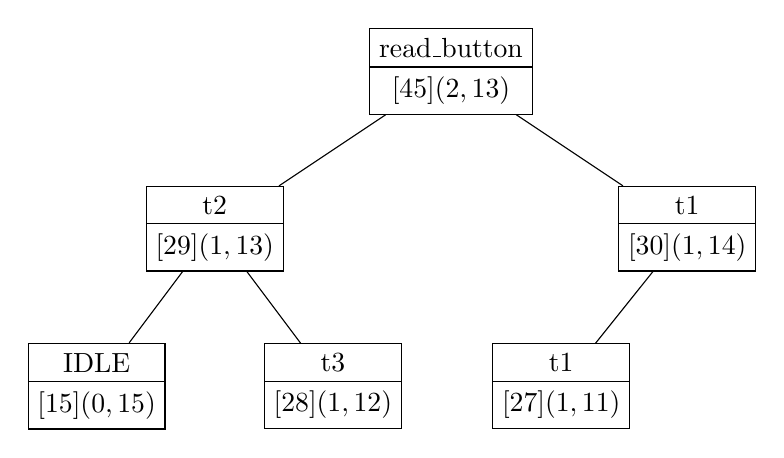
\begin{tikzpicture}[task/.style={rectangle split,rectangle split parts=2,rectangle split draw splits=true,draw}]
   \node[task] (rb) at (0,0) {\nodepart{one} read_button \nodepart{two}$[45](2,13)$};
   \node[task] (t2) at (-3,-2) {\nodepart{one} t2 \nodepart{two}$[29](1,13)$};
   \node[task] (idle) at (-4.5,-4) {\nodepart{one} IDLE \nodepart{two}$[15](0,15)$};
   \node[task] (t3) at (-1.5,-4) {\nodepart{one} t3 \nodepart{two}$[28](1,12)$};
   \node[task] (t1-0) at (3,-2) {\nodepart{one} t1 \nodepart{two}$[30](1,14)$};
   \node[task] (t1-1) at (1.4,-4) {\nodepart{one} t1 \nodepart{two}$[27](1,11)$};
   \draw (rb) -- (t2);
   \draw (rb) -- (t1-0);
   \draw (t2) -- (idle);
   \draw (t2) -- (t3);
   \draw (t1-0) -- (t1-1);
   \end{tikzpicture}
   \caption{Binary heap tree from the example of \ref{sec:readylist}}
   \label{fig:bintree}
\end{figure}

%!TEX root = ./main.tex

\chapter{Building a Trampoline application}

An application using trampoline RTOS is made of a set of source files (C/C++) and a set of oil files (.oil). An oil file allows to define the properties of the different objects handled by the RTOS (tasks, resources, alarms, ...).

\note{Trampoline is a static RTOS, all objects are defined at compile time}

The build phase requires a first step to read these OIL files and transform them into data structures (.c/.h files) for the compilation step. This first operation is done with the tool \goil, provided with Trampoline (Figure \ref{fig:filesbis}).

\begin{figure}[htbp]
    \centering
	\begin{adjustbox}{width=.7\linewidth,keepaspectratio}
		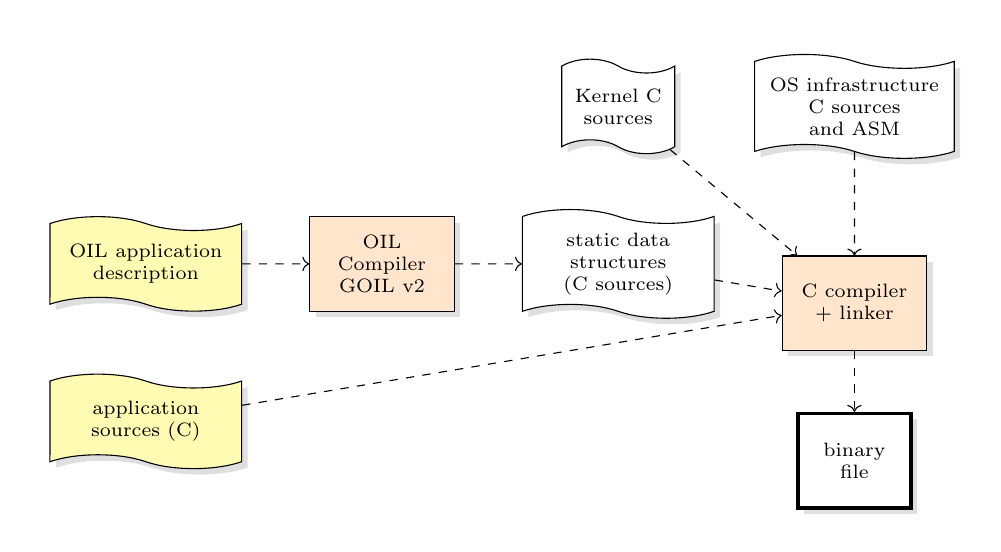
\begin{tikzpicture}[
    manager/.style={draw,fill=white,drop shadow={opacity=0.25},font=\scriptsize, text width=1.6cm, text centered, minimum height=1.2cm},
    exe/.style={draw, very thick,fill=white,drop shadow={opacity=0.25},font=\scriptsize, text width=1.2cm, text centered, minimum height=1.2cm},
    src/.style={draw,tape,fill=white,drop shadow={opacity=0.25},font=\scriptsize, text width=1.2cm, text centered, minimum height=1.2cm, tape bend top=out and in, tape bend bottom=out and in},
    srclarge/.style={draw,tape,fill=white,drop shadow={opacity=0.25},font=\scriptsize, text width=2.3cm, text centered, minimum height=1.2cm, tape bend top=out and in, tape bend bottom=out and in}
    ]
        %cadre (car ça dépasse)
\draw[line width=0pt, white] (-0.5,-3.3) rectangle (11.5,3);

    %\draw[fill=gray!30,drop shadow] (0,0) rectangle (10.2,4);
    %\node[,color=red!50,font=\tiny] at (1,1.15) {OS generation process};
    %\node[,color=red!50,font=\tiny] at (1,0.85) {Application generation process};
    %\node[src] (sdmlsrc)          at (1,4)  {SDML Description};
    %\node[manager] (sdmlcompiler) at (4,4)  {SDML Compiler};
    \node[src] (oskernel)         at (7,2)  {Kernel C sources};
    \node[srclarge] (osinfra)     at (10,2) {OS infrastructure\\C sources and ASM};
    %\node[src,text width=2.7cm] (template)	at (4,2)  { System configuration \\ templates};
    \node[src,,text width=2.2cm,fill=yellow!30] (oil)		at (1,0)  { OIL application description};
    \node[src,,text width=2.2cm,fill=yellow!30] (appli)            at (1,-2)  {application sources (C)};
    \node[src,text width=2.2cm] (applidesc)        at (7,0)  {static data structures  \\(C sources)};
    \node[manager,fill=orange!20] (goil)         at (4,0)  {OIL Compiler\\ GOIL v2};
    \node[manager,fill=orange!20] (c)            at (10,-0.5)  {C compiler + linker };
    \node[exe] (exe)              at (10,-2.5)  {binary file};
    %\path (sdmlsrc) edge [dashed,->] (sdmlcompiler);
    %\path (sdmlcompiler) edge [dashed,->] (oskernel);
    \path (oskernel) edge [dashed,->] (c);
    \path (osinfra) edge [dashed,->] (c);
    \path (applidesc) edge [dashed,->] (c);
    \path (appli) edge [dashed,->] (c);
    %\path (sdmlcompiler) edge [dashed,->] (template);
    \path (oil) edge [dashed,->] (goil);
    %\path (template) edge [dashed,->] (goil);
    \path (goil) edge [dashed,->] (applidesc);
    \path (c) edge [dashed,->] (exe);
    %\draw [thick,dashed,color=red!50] (-1,1) -- (12,1);
    %\draw [dashed,->] ($ (messages.south) + (2mm,0) $) -- ++(0,-4mm) -- ($ (events.south) + (0,-4mm) $) -- (events.south);
    %\draw [dashed,->] ($ (messages.south) - (2mm,0) $) -- ++(0,-6mm) -- ($ (tasks.south) + (0,-6mm) $) -- (tasks.south);
    %\draw [dashed,->] ($ (alarms.south) + (2mm,0) $) -- ++(0,-2mm) -- ($ (tasks.south) + (-2mm,-2mm) $) -- ($ (tasks.south) + (-2mm,0) $);
    %\path (alarms) edge [dashed,->] (events);
    %\path (events) edge [dashed,->] (scheduler);
    %\path (tasks) edge [dashed,->] (scheduler);
    %\path (interrupts) edge [dashed,->] (scheduler);
    %\path (resources) edge [dashed,->] (scheduler);
\end{tikzpicture}
	\end{adjustbox}
\caption{Trampoline Application: from source to binary}
	\label{fig:filesbis}
\end{figure}

In addition to the generation of static data structures, \goil\ is able to generate other files, such as those for the definition of memory mapping (link script), tools for debugging (see \ref{chap:trace}), or tools for the compilation of the application. This chapter deals with the generation of the application.

\section{Main OIL file}

To build the application, some additional information is needed, defined in the sub-attribute \oilattr{CPU->OS->BUILD}. Example for ARM Cortex-M target:

\lstset{language=OIL}
\begin{lstlisting}
CPU blink {
  OS config { 
    BUILD = TRUE {
      TRAMPOLINE_BASE_PATH = "/opt/trampoline";
      APP_SRC = "blink.c";
      APP_NAME = "blink_exe";
      CFLAGS  = "-O0";
      LDFLAGS = "-Map=blink.map";
      COMPILER = "arm-none-eabi-gcc";
      ASSEMBLER = "arm-none-eabi-as";
      LINKER = "arm-none-eabi-ld";
      COPIER = "arm-none-eabi-objcopy";
      SYSTEM = PYTHON;
    };
  ..
\end{lstlisting}

\note{For each target, at least one example is provided in the tree structure \file{examples/}. This is a good starting point.}

This attribute is specific to Trampoline, it contains several sub-attributes to build the application (cross-compiler, flags, source files, …):
\begin{itemize}
	\item \oilattr{TRAMPOLINE_BASE_PATH}: The path to the root of Trampoline. Required
	\item \oilattr{APP_SRC}, \oilattr{APP_CPPSRC} give respectively the C and C++ source files of the application.
	\item \oilattr{CFLAGS}, \oilattr{CPPFLAGS}, \oilattr{ASFLAGS}, \oilattr{LDFLAGS} define the flags to give to the compiler for respectively C, C++, assembly, linker phase. \oilattr{COMMONFLAGS} gives flags for both c,C++and asm source files.
	\item \oilattr{APP_NAME} define the name of the output binary file (to flash)
	\item \oilattr{COMPILER}, \oilattr{CPPCOMPILER}, \oilattr{ASSEMBLER}, \oilattr{LINKER} and \oilattr{COPIER} are the tools (cross compiler collection) related to the C compiler, C++ compiler, assembler, linker and copier (as the GNU tool objcopy)
	\item \oilattr{SYSTEM} defines the build tool in use. It can be either \oilattr{PYTHON} (default) to generate a set of python scripts, or \oilattr{CMAKE} to use the CMake build tool. See section \ref{sec:buildsystem}.
\end{itemize}

As this description is in OIL language, if a sub-attribute is defined twice, then it will be accumulated. For instance:
\lstset{language=OIL}
\begin{lstlisting}
  APP_SRC = "blink.c";
  APP_SRC = "file2.c";
\end{lstlisting}
is equivalent to:
\begin{lstlisting}
  APP_SRC = "blink.c file2.c";
\end{lstlisting}

\section{Build system}
\label{sec:buildsystem}
2 build system are available for Trampoline, defined in the sub-attribute \oilattr{CPU->OS->BUILD->SYSTEM}:
\begin{itemize}
	\item \oilattr{PYTHON} is a set of python script
	\item \oilattr{CMAKE} is a set of CMake files 
\end{itemize}

\subsection{Python build}
The python system generates 2 files \file{build.py} and \file{make.py}. The script will take into account all the dependancies. For example, modifying an object in the oil file will result in calling goil (and generating again the \file{build.py} file again), before doing the rest of the build step. As a result, \goil\ should be called only once (bootstrap), and then \com{./make.py} will do all the stuff.
A basic run is (from \file{examples/cortex/armv7em/stm32f303/Nucleo-32/blink})
\begin{verbatim}
% goil --target=cortex/armv7em/stm32f303 --templates=../../../../../../goil/templates/ blink.oil
Created 'blink/tpl_dispatch_table.c'.
Created 'blink/tpl_invoque.S'.
Created 'blink/tpl_os.h'.
Created 'blink/tpl_service_ids.h'.
Created 'build.py'.
Created 'make.py'.
Created 'blink/tpl_app_custom_types.h'.
Created 'blink/tpl_app_config.c'.
Created 'blink/tpl_app_config.h'.
Created 'blink/tpl_app_define.h'.
Created 'blink/MemMap.h'.
Created 'blink/Compiler.h'.
Created 'blink/Compiler_Cfg.h'.
Created 'blink/script.ld'.
Created 'blink/AsMemMap.h'.
Created 'blink/tpl_static_info.json'.
Created 'blink/tpl_vectors.c'.
Created 'blink/tpl_primary_irq.S'.
Created 'blink/cmsis_wrapper.h'.
Created 'blink/tpl_external_interrupts.c'.
Created 'blink/tpl_app_interrupts.c'.
Created 'blink/tpl_cortex_definitions.h'.
Created 'blink/stm_structure.c'.
executing plugin gdb_commands.goilTemplate
Created '/home/mik/prog/trampoline/examples/cortex/armv7em/stm32f303/Nucleo-32/blink/build/blink.oil.dep'.
No warning, no error.
\end{verbatim}
Then, we call the python script \com{./make.py}:
\begin{verbatim}
-> % ./make.py 
Nothing to make.
Making "build/os" directory
[  3%] Compiling ../../../../../../os/tpl_os_kernel.c
[  6%] Compiling ../../../../../../os/tpl_os_timeobj_kernel.c
…
[ 96%] Compiling ../../../../../../machines/cortex/armv7em/stm32f303/tpl_trace.c
[100%] Linking blink_exe
		   Generating binary blink_exe.bin from blink_exe	
\end{verbatim}

In most cases, an additional target has been defined to flash the application (see section \ref{sec:additionnalTarget}). For Cortex-M targets, this is \com{./make.py burn}.

\subsection{CMake build system}

The CMake build system generates 2 text based files:
\begin{itemize}
	\item \file{CMakeLists.txt} is the main project file
	\item \file{blink/compiler.cmake} (if project is defined in \file{blink.oil}) defines cross-compiler definitions.
\end{itemize}

The bootstrap using \goil\ is the same as in PYTHON:
\begin{verbatim}
% goil --target=cortex/armv7em/stm32f303 --templates=../../../../../../goil/templates/ blink.oil
Created 'blink/tpl_dispatch_table.c'.
Created 'blink/tpl_invoque.S'.
Created 'blink/tpl_os.h'.
Created 'blink/tpl_service_ids.h'.
Created 'CMakeLists.txt'.
Created 'blink/compiler.cmake'.
Created 'blink/tpl_app_custom_types.h'.
Created 'blink/tpl_app_config.c'.
Created 'blink/tpl_app_config.h'.
Created 'blink/tpl_app_define.h'.
Created 'blink/MemMap.h'.
Created 'blink/Compiler.h'.
Created 'blink/Compiler_Cfg.h'.
Created 'blink/script.ld'.
Created 'blink/AsMemMap.h'.
Created 'blink/tpl_static_info.json'.
Created 'blink/tpl_vectors.c'.
Created 'blink/tpl_primary_irq.S'.
Created 'blink/cmsis_wrapper.h'.
Created 'blink/tpl_external_interrupts.c'.
Created 'blink/tpl_app_interrupts.c'.
Created 'blink/tpl_cortex_definitions.h'.
Created 'blink/stm_structure.c'.
executing plugin gdb_commands.goilTemplate
Created '/home/mik/prog/trampoline/examples/cortex/armv7em/stm32f303/Nucleo-32/blink/build/blink.oil.dep'.
No warning, no error.
\end{verbatim}

Then, the command to generate the binary are the standard way, except a special attention to define the correct cross-compiler when calling \tool{cmake}, using the generated cross-compiler access: \com{cmake -D CMAKE_TOOLCHAIN_FILE=../blink/compiler.cmake ..}

\note{These commands are defined in comments in the head of \file{CMakeLists.txt}.}

\begin{verbatim}
% cd build    
% cmake -D CMAKE_TOOLCHAIN_FILE=../blink/compiler.cmake ..
-- The C compiler identification is GNU 9.3.1
-- The CXX compiler identification is GNU 9.4.0
-- Detecting C compiler ABI info
-- Detecting C compiler ABI info - done
-- Check for working C compiler: /opt/gcc-arm/bin/arm-none-eabi-gcc - skipped
-- Detecting C compile features
-- Detecting C compile features - done
-- Detecting CXX compiler ABI info
-- Detecting CXX compiler ABI info - done
-- Check for working CXX compiler: /usr/bin/g++ - skipped
-- Detecting CXX compile features
-- Detecting CXX compile features - done
-- The ASM compiler identification is GNU
-- Found assembler: /opt/gcc-arm/bin/arm-none-eabi-gcc
-- Configuring done
-- Generating done
-- Build files have been written to: /home/mik/prog/trampoline/examples/cortex/armv7em/stm32f303/Nucleo-32/blink/build
-> % make
Scanning dependencies of target blink_exe
[  3%] Building C object CMakeFiles/blink_exe.dir/blink.c.obj
[  6%] Building C object CMakeFiles/blink_exe.dir/home/mik/
...
[ 96%] Linking C executable blink_exe
[100%] Built target blink_exe
\end{verbatim}

In most cases, an additional target has been defined to flash the application (see section \ref{sec:additionnalTarget}). For Cortex-M targets, this is \com{make burn}.

\warning{If the oil file is updated, the build system will call \goil. \goil\ may update \file{CMakeLists.txt}, but this modification will not be taken into account during this pass. In that case, the command \com{make} should be run twice to get a correct behavior.}

The interest of using CMake is that several IDEs are based on this system for the project management (Qt Creator{\footnote{https://www.qt.io/product/development-tools}}, VS Code{footnote{https://code.visualstudio.com/}}, ...). Therefore, we can take advantage of the features of these editors (code completion, navigation between files, ...)

A special case is for VS Code editor. With an additional sub-atribute, a \file{.vscode/} directory is generated (if it does not exist yet), so that the debugger is well configured. In that way, you can directly compile and debug from the editor.
It runs for some Cortex-M based target at this date (STM32).
\lstset{language=OIL}
\begin{lstlisting}
 SYSTEM = CMAKE { VSCODE=TRUE; };
\end{lstlisting}

\section{Goil related features}

Many parts of the build system are generated for \goil\ templates. This section introduces these features.

\subsection{Compilation flags}

Some flags may be defined globally for a specific target. It can be retrieved in the \goil\ templates, in the \file{config/} subfolders. The file is named \file{buildOptions.oil}. For instance, on ARM Cortex-M4 (armv7em ISA), the path is \file{goil/templates/config/cortex/armv7em/buildOptions.oil}.
begin
Some other flags can be added directly in the main \file{config.oil} file in the templates.

\subsection{Additionnal files}

Depending on the target, additional files may need to be compiled. For example, for the \posix\ target, the C files located in the \file{machines/posix} directory must be compiled to enable Trampoline and the application to run in a Unix process. The list of required files is given in one or many OIL objects located along the path in the \file{config} subdirectory of the template directory.

For example, for the target \posix, the list of additional files is as follows:

\begin{lstlisting}[language=OIL]
PLATFORM_FILES posix_port {
    PATH = "posix";
    CFILE = "tpl_machine_posix.c";
    CFILE = "tpl_viper_interface.c";
    CFILE = "tpl_posix_autosar.c";
    CFILE = "tpl_posix_irq.c";
    CFILE = "tpl_posix_context.c";
    CFILE = "tpl_posixvp_irq_gen.c";
};

PLATFORM_FILES posix_port_trace {
    IF = TRACE;
    PATH = "posix";
    CFILE = "tpl_trace.c";
};
\end{lstlisting}

The first object, \lstinline{posix_port}, lists the files that are always required, and the second, \lstinline{posix_port_trace}, lists the file \file{tpl_trace.c} that is required if trace is enabled.

A \oilobj{PLATFORM_FILES} object has the following attributes:

\begin{description}
\item[\texttt{PATH}] is mandatory. It indicates in which directory, relative to the \file{machines} directory, the files are located;
\item[\texttt{CFILE}] gives a C file to be compiled. Several \oilattr{CFILE} attributes may be present;
\item[\texttt{CPPFILE}] gives a C++ file to be compiled. Several \oilattr{CPPFILE} attributes may be present;
\item[\texttt{ASFILE}] gives a assembly language file to be compiled. Several \oilattr{ASFILE} attributes may be present;
\item[\texttt{IF}] refers to a Boolean attribute of the OS object. If this attribute is \oilval{TRUE}, the files are compiled, otherwise they are not.
\end{description}

For example, the following statement indicates that the file \file{machines/tpl_trace.c} should be compiled if the \oilattr{TRACE} attribute of the \oilattr{OS} object is \oilval{TRUE}.

\begin{lstlisting}[language=OIL]
PLATFORM_FILES posix_port_trace {
    IF = TRACE;
    PATH = "posix";
    CFILE = "tpl_trace.c";
};
\end{lstlisting}


\subsection{Libraries}



\subsection{Additionnal build target}
\label{sec:additionnalTarget}
TODO


\part{Trampoline RTOS internals}

%!TEX root = ./trampoline.tex

\chapter{System generation and compilation}

Trampoline is a static operating system. This means all the objects (tasks, ISR, ...) are known at compile time. This way, an application is made of tasks' code and ISRs' code, application data, and statically initialized descriptor for each object the operating system manages. A system generation tool, like \goil, generates these descriptors in C files from an application configuration described in OIL or in XML. After that the Trampoline source code, the generated files and the application source code are compiled and linked together to produce an executable file as shown in figure \ref{fig:buildtrampoline}.

\begin{figure}[htbp] %  figure placement: here, top, bottom, or page
   \centering
   \includegraphics[width=4.5in]{pictures/buildProcess.pdf} 
   \caption{\textbf{Build process of an application with Trampoline.} Starting from the left, the .c and .h corresponding to the application description given in OIL (or XML) are generated by \goil\ (or another system generation tool, for instance an Autosar compliant one) and compiled using a C compiler. Trampoline source files are compiled too and include .h from the description for configuration purpose (see section \ref{sec:configmacros}). Application files are compiled and include .h files from Trampoline. All the object files are then linked together using an optional link script generated by \goil\ or provided with the application.}\label{fig:buildtrampoline}
\end{figure}

\section{The generated files}
\label{sec:generatedfiles}

The following files are generated by \goil\ from the OIL file or should be generated if you use a different system configuration tool. More information may be found in part \ref{part:goil}.

\rowcolors{1}{white}{light-gray}
\begin{longtableii}{l|p{3.5in}}{file}{File name}{Usage}

\lineii{tpl_app_define.h\index{tpl_app_define.h}}{This file contains all the configuration macros (see section \ref{sec:configmacros}) and is included in all the Trampoline files to trigger conditional compilation. \goil\ generates this file using the \file{tpl_app_define_h.goilTemplate} template file.}

\lineii{tpl_app_config.h\index{tpl_app_config.h}}{This file contains the declarations of the constants and functions required by the OSEK and Autosar standard (like OSMAXALLOWEDVALUE_x, OSTICKSPERBASE_x or OSMINCYCLE_x constants for counter x). \goil\ generates this file using the \file{tpl_app_config_h.goilTemplate} template file.}

\lineii{tpl_app_config.c\index{tpl_app_config.c}}{This file contains the definitions of the constants and functions required by the OSEK and Autosar standard and the definitions of object descriptors used by Trampoline (see section \ref{sec:structs}) \goil\ generates this file using the \file{tpl_app_config_c.goilTemplate} template file.}

\lineii{tpl_app_custom_types.h\index{tpl_app_custom_types.h}}{Some data types used by Trampoline are not statically defined. They are generated to fit size or performance criterions. For instance, the type used for a TaskType may be a byte if there is less than 256 tasks in the system and a word otherwise. This file defined these data types.}

\lineii{tpl_service_ids.h\index{tpl_service_ids.h}}{This file is generated only if Trampoline is compiled with service calls implemented using a system call. It contains all the identifiers of the services used by the application according to the configuration. \goil\ generates this file using the \file{tpl_service_ids_h.goilTemplate} template file.}

\lineii{tpl_dispatch_table.c\index{tpl_dispatch_table.c}}{This file is generated only if Trampoline is compiled with service calls implemented using a system call. It contains the dispatch table definition. See section \ref{sec:dispatchtable}. \goil\ generates this file using the \file{tpl_dispatch_table_c.goilTemplate} template file.}

\lineii{tpl_invoque.S\index{tpl_invoque.S}}{This file is generated only if Trampoline is compiled with service calls implemented using a system call. It contains the API functions for system services. See section \ref{sec:invoque}. The extension (here .S) may change according to the assembler used. \goil\ generates this file using the \file{tpl_invoque.goilTemplate} and \file{service_call.goilTemplate} template files.}

\lineii{MemMap.h\index{MemMap.h}}{This file is generated only if memory mapping is enabled. It contains macros for compiler abstraction memory mapping of functions and data as defined in the Autosar standard \cite{autosar31memorymapping}. \goil\ generates this file using the \file{MemMap_h.goilTemplate} template file.}

\lineii{Compiler.h\index{Compiler.h}}{This file is generated only if memory mapping is enabled. It contains macros for the compiler abstraction of functions and pointer qualifier as defined in the Autosar standard \cite{autosar31compilerabstraction}. \goil\ generates this file using the \file{Compiler_h.goilTemplate} template file.}

\lineii{Compiler_Cfg.h\index{Compiler_Cfg.h}}{This file is generated only if memory mapping is enabled. It contains macros for the compiler abstraction configuration as defined in the Autosar standard \cite{autosar31compilerabstraction}. \goil\ generates this file using the \file{Compiler_Cfg_h.goilTemplate} template file.}

\lineii{script.ld\index{script.ld}}{This file is generated only if memory mapping is enabled. It contains a link script to map the executable in the target memory. \goil\ generates this file using the \file{script.goilTemplate} template file.}

\end{longtableii}

The following sections give details about the content of these files.

\section{The Configuration Macros}
\label{sec:configmacros}

Trampoline can be compiled with various options. These options are controlled by setting the appropriate preprocessor configuration macros%
\index{Configuration macros}.
These macros are usually set by \goil
using the template found in \file{tpl_app_define_h.goilTemplate} file to produce the \file{tpl_app_define.h}\index{tpl_app_define.h} file that is included by the files of Trampoline. However, a different generation tool may be used and it should comply to the specification presented in the following tables. When Trampoline is compiled, the coherency and consistency of the configuration macros are checked, by using the preprocessor macros located in the \file{tpl_config_check.h} file, to ensure they correspond to a supported configuration.

3 kinds of configuration macros are used: boolean macros, numerical macros, symbol macros and string macros. Boolean macros may take 2 values: YES or NO. All macros should be defined, Trampoline does not use the \lstinline[language=C]{#ifdef} or \lstinline[language=C]{\#ifndef} scheme to limit the occurrences of unwanted misconfigurations except to prevent multiple inclusions of the same header file.

\subsection{Number of objects macros}

These macros gives the number of objects of each kind (tasks, ISRs, resources, \ldots) and other values. They are used in Trampoline to check the validity of the various identifiers and to define tables of the corresponding size:
 
\rowcolors{1}{white}{light-gray}
\begin{longtableiii}{l|l|p{3.1in}}{var}{Macro}{Kind}{Effect}
  \lineiii{\idxconfflag{PRIO_LEVEL_COUNT}}
  {Integer}
  {The number of priority levels used in the system.}
  \lineiii{\idxconfflag{TASK_COUNT}}
  {Integer}
  {The number of tasks (basic and extended) used in the system.}
  \lineiii{\idxconfflag{EXTENDED_TASK_COUNT}}
  {Integer}
  {The number of extended tasks used in the system.}
  \lineiii{\idxconfflag{ISR_COUNT}}
  {Integer}
  {The number of ISR category 2 used in the system.}
  \lineiii{\idxconfflag{ALARM_COUNT}}
  {Integer}
  {The number of alarms used in the system.}
  \lineiii{\idxconfflag{RESOURCE_COUNT}}
  {Integer}
  {The number of resources used in the system.}
  \lineiii{\idxconfflag{SEND_MESSAGE_COUNT}}
  {Integer}
  {The number of send messages used in the system.}
  \lineiii{\idxconfflag{RECEIVE_MESSAGE_COUNT}}
  {Integer}
  {The number of receive messages used in the system.}
  \lineiii{\idxconfflag{SCHEDTABLE_COUNT}}
  {Integer}
  {The number of schedule tables used in the system. This macros is only used when WITH_AUTOSAR is set to YES.}
  \lineiii{\idxconfflag{COUNTER_COUNT}}
  {Integer}
  {The number of counters used in the system. This macros is only used when WITH_AUTOSAR is set to YES.}
  \lineiii{\idxconfflag{APP_COUNT}}
  {Integer}
  {The number of OS applications used in the system. This macros is only used when WITH_AUTOSAR is set to YES.}
  \lineiii{\idxconfflag{TRUSTED_FCT_COUNT}}
  {Integer}
  {The number of trusted functions used in the system. This macros is only used when WITH_AUTOSAR is set to YES.}
  \lineiii{\idxconfflag{RES_SCHEDULER_PRIORITY}}
  {Integer}
  {The priority of the RES_SCHEDULER resource. This should be equal to the highest priority among the tasks.}
\end{longtableiii}

\subsection{Error Handling Macros}

Error handling related macros are used to configure what kind of error Trampoline checks and what extra processing is done when an error is encountered. The following macros are available:

\rowcolors{1}{white}{light-gray}
\begin{longtableiii}{l|l|p{2.5in}}{var}{Macro}{Kind}{Effect}
  \lineiii{\idxconfflag{WITH_OS_EXTENDED}}
  {Boolean}
  {When set to YES, Trampoline system services perform error checking on their arguments. \var{WITH_OS_EXTENDED} is set to YES with a \var{STATUS} = EXTENDED and is set to NO with a \var{STATUS} = BASIC in the oil OS object.}
  \lineiii{\idxconfflag{WITH_ERROR_HOOK}\label{sec:errorhook}}
  {Boolean}
  {When set to YES, the \function{ErrorHook()} function is called if an error occurs. \var{WITH_ERROR_HOOK} is set to YES/NO with a \var{ERRORHOOK} = TRUE/FALSE in the oil OS object.}
  \lineiii{\idxconfflag{WITH_USEGETSERVICEID}}
  {Boolean}
  {When set to YES, Trampoline system services store the id of the current service. This id may be retrieved in the \function{ErrorHook()} function by using the \function{OSErrorGetServiceId()} macro. \var{WITH_USEGETSERVICEID} is set to YES/NO with a \var{USEGETSERVICEID} = TRUE/FALSE in the oil OS object.}
  \lineiii{\idxconfflag{WITH_USEPARAMETERACCESS}}
  {Boolean}
  {When set to YES, Trampoline system services store the arguments of the current service. These arguments may be retrieved in the \function{ErrorHook()} function by using the ad-hoc access macros (see \ref{sec:errorhook}). \var{WITH_USEPARAMETERACCESS} is set to YES/NO with a \var{USEPARAMETERACCESS} = TRUE/FALSE in the oil OS object.}
  \lineiii{\idxconfflag{WITH_COM_ERROR_HOOK}}
  {Boolean}
  {When set to YES, the communication error hook is called when error occurs in the communication sub-system. This macro is only available when WITH_COM is set to true.}
  \lineiii{\idxconfflag{WITH_COM_USEGETSERVICEID}}
  {Boolean}
  {When set to YES, Trampoline/COM system services store the id of the current service. This id may be retrieved in the \function{COMErrorHook()} function by using the \function{COMErrorGetServiceId()} macro. \var{WITH_COM_USEGETSERVICEID} is set to YES/NO with a \var{COMUSEGETSERVICEID} = TRUE/FALSE in the oil COM object.}
  \lineiii{\idxconfflag{WITH_COM_USEPARAMETERACCESS}}
  {Boolean}
  {When set to YES, Trampoline/COM system services store the arguments of the current service. These arguments may be retrieved in the \function{COMErrorHook()} function by using the ad-hoc access macros (see \ref{sec:comerrorhook}). \var{WITH_COM_USEPARAMETERACCESS} is set to YES/NO with a \var{COMUSEPARAMETERACCESS} = TRUE/FALSE in the oil COM object.}
  \lineiii{\idxconfflag{WITH_COM_EXTENDED}}
  {Boolean}
  {When set to YES, Trampoline/COM system services perform error checking on their arguments. \var{WITH_COM_EXTENDED} is set to YES with a \var{COMSTATUS} = EXTENDED and is set to NO with a \var{COMSTATUS} = BASIC in the oil COM object.}
\end{longtableiii}

\subsection{Protection Macros}

Protection macros deal with protection facility provided by the Autosar standard. The following Macros are available:

\rowcolors{1}{white}{light-gray}
\begin{longtableiii}{l|l|p{2.9in}}{var}{Macro}{Kind}{Effect}
  \lineiii{\idxconfflag{WITH_MEMORY_PROTECTION}}
  {Boolean}
  {When set to YES, Trampoline enables the memory protection facility. This is only supported on some ports (MPC5510 and ARM9 at time of writing). Memory protection requires the memory mapping and the use of system call. \var{WITH_MEMORY_PROTECTION} is set to YES/NO with the MEMORY_PROTECTION attribute of MEMMAP object (see \ref{sec:memmap}) set to TRUE/FALSE.}
  \lineiii{\idxconfflag{WITH_TIMING_PROTECTION}}
  {Boolean}
  {When set to YES, Trampoline enables the timing protection facility. \var{WITH_TIMING_PROTECTION} is set to YES if the \var{AUTOSAR_SC} is 2 or 4 (see \ref{sec:autosarsc}) and a least one of the objects specifies a timing protection related attribute in the oil file.}
  \lineiii{\idxconfflag{WITH_PROTECTION_HOOK}\label{sec:protectionhook}}
  {Boolean}
  {When set to YES, Trampoline calls the ProtectionHook() with the appropriate argument when a protection fault occurs. \var{WITH_PROTECTION_HOOK} is set to YES with a \var{PROTECTIONHOOK} = TRUE in the oil OS object.}
  \lineiii{\idxconfflag{WITH_STACK_MONITORING}}
  {Boolean}
  {When set to YES, Trampoline enables the stack monitoring. Each time a context switch occurs, the stack pointer is checked. If the stack pointer is outside the stack zone of the process, a fault occurs. \var{WITH_STACK_MONITORING} is set to YES with a \var{STACKMONITORING} = TRUE in the oil OS object.}
\end{longtableiii}

\subsection{Hook call macros}

Hook call macros control whether a hook is called or not. The following Macros are available:

\rowcolors{1}{white}{light-gray}
\begin{longtableiii}{l|l|p{3.1in}}{var}{Macro}{Kind}{Effect}
  \lineiii{\idxconfflag{WITH_ERROR_HOOK}}
  {Boolean}
  {see \ref{sec:errorhook}}
  \lineiii{\idxconfflag{WITH_PRE_TASK_HOOK}}
  {Boolean}
  {When set to YES, each time a task is scheduled, the function PreTaskHook() is called.
  \var{WITH_PRE_TASK_HOOK} is set to YES/NO with a \var{PRETASKHOOK} = TRUE/FALSE
  in the oil OS object.}
  \lineiii{\idxconfflag{WITH_POST_TASK_HOOK}}
  {Boolean}
  {When set to YES, each time a task is descheduled, the function PostTaskHook() is called.
  \var{WITH_POST_TASK_HOOK} is set to YES/NO with a \var{POSTTASKHOOK} = TRUE/FALSE
  in the oil OS object.}
  \lineiii{\idxconfflag{WITH_STARTUP_HOOK}}
  {Boolean}
  {When set to YES, the function StartupHook() is called within the StartOS service.
  \var{WITH_STARTUP_HOOK} is set to YES/NO with a \var{STARTUPHOOK} = TRUE/FALSE
  in the oil OS object.}
  \lineiii{\idxconfflag{WITH_SHUTDOWN_HOOK}}
  {Boolean}
  {When set to YES, the function ShutdownHook() is called within the ShutdownOS service.
  \var{WITH_SHUTDOWN_HOOK} is set to YES/NO with a \var{SHUTDOWNHOOK} = TRUE/FALSE
  in the oil OS object.}
  \lineiii{\idxconfflag{WITH_PROTECTION_HOOK}}
  {Boolean}
  {see \ref{sec:protectionhook}}
\end{longtableiii}

\subsection{Miscellaneous macros}

Here are the other available macros:

\rowcolors{1}{white}{light-gray}
\begin{longtableiii}{l|l|p{2.6in}}{var}{Macro}{Kind}{Effect}
  \lineiii{\idxconfflag{WITH_USERESSCHEDULER}}
  {Boolean}
  {When set to YES, the RES_SCHEDULER resource is used by at least one process. \var{WITH_USERESSCHEDULER} is set to YES/NO with a \var{USERESSCHEDULER} = TRUE/FALSE
  in the oil OS object.}
  \lineiii{\idxconfflag{WITH_SYSTEM_CALL}}
  {Boolean}
  {When set to YES, services are called by the mean of a system call, also known as a software interrupt (see section \ref{sec:systemcall}).
  \var{WITH_SYSTEM_CALL} is set to YES/NO according to the target architecture and requires a memory mapping}
  \lineiii{\idxconfflag{WITH_MEMMAP}}
  {Boolean}
  {When set to YES, a memory mapping is used: A \file{MemMap.h} files giving the available memory segments is included and should be generated or provided by the user. \goil\ generates such a file.
  \var{WITH_MEMMAP} is set to YES/NO with a \var{MEMMAP} = TRUE/FALSE
  in the oil OS object.}
  \lineiii{\idxconfflag{WITH_COMPILER_SETTINGS}}
  {Boolean}
  {When set to YES, the compiler dependent Autosar macros are used: \file{Compiler.h} and \file {Compiler_Cfg.h} files are includes and should generated or provided by the user. \goil\ generates these  files if \var{MEMMAP} is TRUE and the \var{COMPILER} sub-attribute is set.}
  \lineiii{\idxconfflag{WITH_AUTOSAR}}
  {Boolean}
  {When set to YES, Trampoline contains additional system services, code and declarations related to the Autosar standard. For instance, the counter descriptor includes the counter type (hardware or software).
  \var{WITH_AUTOSAR} is set to YES/NO when at least an Autosar object is present in the system configuration (oil file for instance).}
  \lineiii{\idxconfflag{TRAMPOLINE_BASE_PATH}}
  {String}
  {The path to Trampoline root directory.}
  \lineiii{\idxconfflag{AUTOSAR_SC}}
  {Integer}
  {The Autosar scalability class\index{Scalability class} ranging from 0 to 4. 0 means OSEK}
  \lineiii{\idxconfflag{WITH_OSAPPLICATION}}
  {Boolean}
  {When set to YES, OS Application\index{OS Application} are used.}
  \lineiii{\idxconfflag{WITH_TRACE}}
  {Boolean}
  {When set to YES, the tracing of the operating system is enabled. Only available if WITH_TRACE is set to YES.}
  \lineiii{\idxconfflag{TRACE_TASK}}
  {Boolean}
  {When set to YES, task (de)scheduling events are traced. Only available if WITH_TRACE is set to YES.}
  \lineiii{\idxconfflag{TRACE_ISR}}
  {Boolean}
  {When set to YES, ISR category 2 (de)scheduling events are traced. Only available if WITH_TRACE is set to YES.}
  \lineiii{\idxconfflag{TRACE_RES}}
  {Boolean}
  {When set to YES, resources get and release are traced. Only available if WITH_TRACE is set to YES.}
  \lineiii{\idxconfflag{TRACE_ALARM}}
  {Boolean}
  {When set to YES, alarm activities are traced. Only available if WITH_TRACE is set to YES.}
  \lineiii{\idxconfflag{TRACE_U_EVENT}}
  {Boolean}
  {When set to YES, user events are traced. Only available if WITH_TRACE is set to YES.}
  \lineiii{\idxconfflag{TRACE_FORMAT}}
  {Symbol}
  {Trace format. A function named tpl_trace_format_\toreplace{trace_format} is expected. Only available if WITH_TRACE is set to YES.}
  \lineiii{\idxconfflag{TRACE_FILE}}
  {String}
  {File name where the trace is stored. Usable on Posix target only. Only available if WITH_TRACE is set to YES.}
  \lineiii{\idxconfflag{WITH_IT_TABLE}}
  {Boolean}
  {When set to YES, the external interrupts are dispatched using a table of fonction pointers.}
  \lineiii{\idxconfflag{WITH_COM}}
  {Boolean}
  {When set to YES, internal communication is used.}
  \lineiii{\idxconfflag{TPL_COMTIMEBASE}}
  {Integer}
  {The COMTIMEBASE expresses in nanoseconds.}
  \lineiii{\idxconfflag{WITH_COM_STARTCOMEXTENSION}}
  {Boolean}
  {When set to YES, the communication extension function is called.}
\end{longtableiii}

\section{Application configuration}

The application configuration is generated by \goil\ using the template found in \file{tpl_app_config_h.goilTemplate} file and \file{tpl_app_config_c.goilTemplate} file to produce the \file{tpl_app_define.h}\index{tpl_app_define.h} and \file{tpl_app_define.c}\index{tpl_app_define.c} files.

\subsection{Counter related constants declaration}

The \file{tpl_app_config.h} files contains the counters related constants: those of the SystemCounter\footnote{the default counter of an OSEK operating system} and those of the counters defined by the user. The SystemCounter constants are located in the generated files because the SystemCounter default attributes may be modified by the user in the OIL or XML file. The constants of a user defined counter are declared as follow:

\begin{lstlisting}[language=C]
extern CONST(tpl_tick, OS_CONST) OSTICKSPERBASE_<counter name>;
extern CONST(tpl_tick, OS_CONST) OSMAXALLOWEDVALUE_<counter name>;
extern CONST(tpl_tick, OS_CONST) OSMINCYCLE_<counter name>;
\end{lstlisting}

Where \toreplace{counter name} is obviously the name given to the counter in the confguration. For the SystemCounter, the following constants are declared:

\begin{lstlisting}[language=C]
extern CONST(tpl_tick, OS_CONST) OSTICKSPERBASE;
extern CONST(tpl_tick, OS_CONST) OSMAXALLOWEDVALUE;
extern CONST(tpl_tick, OS_CONST) OSMINCYCLE;
\end{lstlisting}

\subsection{Events definition}

The \file{tpl_app_config.c} file should contain the event mask definitions. For each event defined in the configuration, the following lines should appear:

\begin{lstlisting}[language=C]
#define API_START_SEC_CONST_UNSPECIFIED
#include "tpl_memmap.h"

#define <event name>_mask <mask value>
CONST(EventMaskType, AUTOMATIC) <event name> = <event name>_mask;

#define API_STOP_SEC_CONST_UNSPECIFIED
#include "tpl_memmap.h"
\end{lstlisting}

Where \toreplace{event name} is the name given to the event in the configuration and \toreplace{mask value} is the value set by the user in the configuration or, when set to AUTO, the value computed by the generation tool.

\subsection{Standard resources definition}

Standard resources need the definition of an identifier used to reference the resource in a system service (\cfunction{GetResource()} and \cfunction{ReleaseResource()}) and an instance of a \ctype{tpl_resource} structure (see \ref{sec:structtplresource}). This is done with the following definitions:

\begin{lstlisting}[language=C]
#define API_START_SEC_CONST_UNSPECIFIED
#include "tpl_memmap.h"

#define <resource name>_id <resource id>
CONST(ResourceType, AUTOMATIC) <resource name> = <resource name>_id;

#define API_STOP_SEC_CONST_UNSPECIFIED
#include "tpl_memmap.h"

#define OS_START_SEC_VAR_UNSPECIFIED
#include "tpl_memmap.h"

VAR(tpl_resource, OS_VAR) <resource name>_rez_desc = {
  /* ceiling priority of the resource */  <resource priority>,
  /* owner previous priority          */  0,
  /* owner of the resource            */  INVALID_PROC_ID,
#if WITH_OSAPPLICATION == YES
  /* OS Application id                */  <resource application id>,
#endif    
  /* next resource in the list        */  NULL
};

#define OS_STOP_SEC_VAR_UNSPECIFIED
#include "tpl_memmap.h"
\end{lstlisting}

Where \toreplace{resource name} is the name given to the resource in the configuration, \toreplace{resource priority} is the priority of the resource that is computed by the generation tool and is the maximum priority of the processes that use the resource and \toreplace{resource application id} is the identifier of the OS Application the resource belongs to. Since this field is protected by \var{WITH_OSAPPLICATION}, it may be leaved empty when no OS Application is used.

\toreplace{resource id} ranges from 0 to the number of standard resources minus 1. Once every standard resource descriptor is defined, a table gathering pointers to the resource descriptors and indexed by the resource id has to be defined. This table is used by system services to get the resource descriptor from the resource id. Suppose 3 standard resource, \var{motor1}, \var{motor2} and \var{dac} has been defined and RES_SCHEDULER is used, the table should be as follow:

\begin{lstlisting}[language=C]
#define OS_START_SEC_CONST_UNSPECIFIED
#include "tpl_memmap.h"
CONSTP2VAR(tpl_resource, AUTOMATIC, OS_APPL_DATA)
tpl_resource_table[RESOURCE_COUNT] = {
  &motor1_rez_desc,
  &motor2_rez_desc,
  &dac_rez_desc,
  &res_sched_rez_desc  
};
#define OS_STOP_SEC_CONST_UNSPECIFIED
#include "tpl_memmap.h"
\end{lstlisting}

\var{\&res_sched_rez_desc}, the pointer to the resource descriptor of RES_SCHEDULER should always be the last element of the table. If RES_SCHEDULER is not used, simply remove it from the table.

\subsection{Tasks definition}

Each task needs an identifier to reference a task un a system service (\cfunction{ActivateTask()}, \cfunction{ChainTask()}, \cfunction{GetTaskState()}, \cfunction{SetEvent()} and \cfunction{GetEvent()}) and the declaration of the task function. The following definitions should appear for each task:

\begin{lstlisting}[language=C]
#define API_START_SEC_CONST_UNSPECIFIED
#include "tpl_memmap.h"

#define <task name>_id <task id>
CONST(TaskType, AUTOMATIC) <task name> = <task name>_id;

#define API_STOP_SEC_CONST_UNSPECIFIED
#include "tpl_memmap.h"

#define APP_Task_<task name>_START_SEC_CODE
#include "tpl_memmap.h"

FUNC(void, OS_APPL_CODE) <task name>_function(void);

#define APP_Task_<task name>_STOP_SEC_CODE
#include "tpl_memmap.h"
\end{lstlisting}

Where \toreplace{task name} is the name given to the task in the configuration and \toreplace{task id} is the identifier of the task computed by the system generation tool. Task ids should range from 0 to the number of tasks minus 1. In addition, id allocation must start with extended tasks first and basic task after. In addition an instance of the static task descriptor must be provided:

\begin{lstlisting}[language=C]
#define OS_START_SEC_CONST_UNSPECIFIED
#include "tpl_memmap.h"
CONST(tpl_proc_static, OS_CONST) <task name>_task_stat_desc = {
  /* context                  */  <task name>_CONTEXT,
  /* stack                    */  <task name>_STACK,
  /* entry point (function)   */  <task name>_function,
  /* internal ressource       */  <internal resource>,
  /* task id                  */  <task name>_id,
#if WITH_OSAPPLICATION == YES
  /* OS application id        */  <application>,
#endif
  /* task base priority       */  <task priority>,
  /* max activation count     */  <task activation>,
  /* task type                */  <task type>
#if WITH_AUTOSAR_TIMING_PROTECTION == YES
  /* pointer to the timing
     protection descriptor    */  ,<timing protection>
#endif
};
#define OS_STOP_SEC_CONST_UNSPECIFIED
#include "tpl_memmap.h"
\end{lstlisting}

Where \toreplace{task name} is the name given to the task in the configuration. \toreplace{internal resource} mays be one of the following:

\begin{itemize}
\item a pointer to the internal resource descriptor (see \ref{sec:internalresource}) if an internal resource has been defined in the configuration;
\item a pointer to the scheduler internal resource if the task has been defined as non-preemptable in the configuration;
\item NULL if none of the above cases apply.
\end{itemize}

\toreplace{application} is the id of the OS Application the task belongs to when OS Application are used or, when they are not used, nothing at all. \toreplace{task priority} is the priority of the task as computed by the \sysgen. \toreplace{task activation} is the maximum number of task activation allowed as defined in the configuration. \toreplace{task type} may be EXTENDED or BASIC. \toreplace{timing protection} is a pointer to the timing protection descriptor or NULL if no timing protection is defined for the task.

Also an instance of the dynamic task descriptor must be provided:

\begin{lstlisting}[language=C]
#define OS_START_SEC_VAR_UNSPECIFIED
#include "tpl_memmap.h"

VAR(tpl_proc, OS_VAR) <task name>_task_desc = {
  /* resources                      */  NULL,
#if WITH_MEMORY_PROTECTION == YES
  /* if > 0 the process is trusted  */  <trusted count>,    
#endif /* WITH_MEMORY_PROTECTION */
  /* activate count                 */  0,
  /* task priority                  */  <task priority>,
  /* task state                     */  <task state>
#if WITH_AUTOSAR_TIMING_PROTECTION == YES
  /* activation allowed             */  ,TRUE
#endif
};

#define OS_STOP_SEC_VAR_UNSPECIFIED
#include "tpl_memmap.h"
\end{lstlisting}

Where \toreplace{task name} is the name given to the task in the configuration. \toreplace{trusted count} is 0 if the task belongs to a non trusted OS Application and 1 if the tasks belongs to a trusted OS Application. \toreplace{task priority} is the priority of the task as computed by the \sysgen. \toreplace{task state} is the initial state of the task and must be set to AUTOSTART or SUSPENDED.

If the task is an EXTENDED one, an event mask descriptor is added:

%\lstdefinelanguage[trampconf]{C}{morecomment=[s][\color{red}]{<}{>}}

\begin{lstlisting}[language=C]
VAR(tpl_task_events, OS_VAR) <task name>_task_evts = {
  /* event set  */ 0,
  /* event wait */ 0
};
\end{lstlisting}

Where \toreplace{task name} is the name given to the task in the configuration.


%!TEX root = ./main.tex

\chapter{Implementation details}

\section{The \var{tpl_kern} structure}

The \var{tpl_kern} structure gathers informations about the \RUNNING\ process and flags to notify if a context switch and/or a context save are needed. It eases the access to these informations when programming in assembly language. The \var{tpl_kern} structure is an instance of the \ctype{tpl_kern_state} type:

\begin{lstlisting}[language=C]
typedef struct 
{
  P2CONST(tpl_proc_static, TYPEDEF, OS_CONST) s_old;
  P2CONST(tpl_proc_static, TYPEDEF, OS_CONST) s_running;
  P2VAR(tpl_proc, TYPEDEF, OS_VAR)            old;
  P2VAR(tpl_proc, TYPEDEF, OS_VAR)            running;
  VAR(int, TYPEDEF)                           running_id;
  VAR(u8, TYPEDEF)                            need_switch;
} tpl_kern_state;
\end{lstlisting}
\documentclass[11pt, oneside]{article}   	% use "amsart" instead of "article" for AMSLaTeX format
\usepackage{geometry}                		% See geometry.pdf to learn the layout options. There are lots.
\geometry{letterpaper}                   		% ... or a4paper or a5paper or ... 
%\geometry{landscape}                		% Activate for for rotated page geometry
%\usepackage[parfill]{parskip}    		% Activate to begin paragraphs with an empty line rather than an indent
\usepackage{graphicx}				% Use pdf, png, jpg, or eps§ with pdflatex; use eps in DVI mode
								% TeX will automatically convert eps --> pdf in pdflatex		
\usepackage{amssymb}
\usepackage[utf8]{inputenc}
\usepackage{listings}
\usepackage{hyperref}
\usepackage{tikz}
\usetikzlibrary{patterns,calc}

\newcommand{\sch}{\lstinline{tpl_sc_handler}}

\title{MSP430X port}
\author{Jean-Luc Béchennec}
%\date{}							% Activate to display a given date or no date

\lstset{% general command to set parameter(s)
	basicstyle=\footnotesize\ttfamily,
	backgroundcolor=\color{lightgray!30},
	frame=single, framerule=0pt
}

\begin{document}
\maketitle

Instruction set of the MSP430X is available in \cite{slau208q} or \cite{slau367o}.

\section{ABI}

In \cite{slaa664} a change has been made in GCC so that it conforms to the ABI defined in \cite{slaa534} and becomes compatible with the proprietary Texas Instruments compiler. So there are two GCC compilers for MSP430: the one that does not conform to the ABI defined by Texas Instruments, \emph{MSPGCC}, and the one that does conform to the ABI, \emph{GCC compiler for MSP}. 

As it is difficult to support both ABIs simultaneously, it was decided to support both ABIs at compile time. A precompiled \emph{MSPGCC} is available in the latest version of Energia\footnote{GCC 4.6.3.}. Energia can be downloaded at {\small\url{https://energia.nu}}. A precompiled \emph{GCC compiler for MSP} is available at {\small\url{http://www.ti.com/tool/msp430-gcc-opensource}}.

In both ABIs the registers used to pass arguments to functions are \lstinline{r12}, \lstinline{r13}, \lstinline{r14} and \lstinline{r15}. In the ABI of \emph{MSPGCC}, \lstinline{r15} is the first argument, \lstinline{r14} the second and so on. If a function returns a value, it is placed in \lstinline{r15}. In the ABI of \emph{GCC compiler for MSP} \lstinline{r12} is the first argument, \lstinline{r13} the second and so on. If a function returns a value, it is placed in \lstinline{r12}.
 No Trampoline service uses more than 3 arguments and therefore \lstinline{r12}, for \emph{MSPGCC} ABI, or \lstinline{r15}, for \emph{GCC compiler for MSP} ABI, is available to pass the service ID into the wrapper.
 
Adapting to both ABIs at compile time is not very complicated. This involves exchanging the use made of the registers \lstinline{r12}, identifying the service, and \lstinline{r15}, the return value of the service and the argument of \lstinline{tpl_run_elected}. This can be done by defining an abstract register to pass the service identifier and an abstract register to return the return value of the service. The register selection can be made using the preprocessor and the macro \lstinline{__GXX_ABI_VERSION} as shown at Figure \ref{lst:macroabi}. This macro is \lstinline{1002} for \emph{MSPGCC} and \lstinline{1011} for \emph{GCC compiler for MSP}. 2 abstract registers are defined: \lstinline{REG_SID} which is \lstinline{r12} in \emph{MSPGCC} ABI and \lstinline{r15} in \emph{GCC compiler for MSP} ABI, and \lstinline{REG_RETARG} which is \lstinline{r15} in \emph{MSPGCC} ABI and \lstinline{r12}  in \emph{GCC compiler for MSP} ABI.

\begin{figure}[h]
\caption{ABI selection with C preprocessor macros}
\begin{lstlisting}
#if __GXX_ABI_VERSION == 1002
/* MSPGCC ABI */
#define MSPGCC_ABI
#define REG_SID r12
#define REG_RETARG r15
#elif __GXX_ABI_VERSION == 1011
/* GCC compiler for MSP ABI */
#define GCCFORMSP_ABI
#define REG_SID r15
#define REG_RETARG r12
#else
#error "Unsupported ABI"
#endif
\end{lstlisting}
\label{lst:macroabi}
\end{figure}

The following table summarizes the use of the registers in both ABIs if we consider all arguments are small enough to be stored in one register. Although \lstinline{r11} is volatile in one of them, for simplification purposes later on, \lstinline{r11} is considered as non-volatile. A preserved register is noted P and a Volatile register is noted V.

\begin{center}
\begin{tabular}{|l|c|c|}
\hline
Register & \emph{MSPGCC} & \emph{GCC compiler for MSP} \\
\hline
\hline
\lstinline|r0| & \multicolumn{2}{c|}{Program Counter, saved on stack by cpu} \\
\hline
\lstinline|r1| & \multicolumn{2}{c|}{Stack Pointer} \\
\hline
\lstinline|r2| & \multicolumn{2}{c|}{Status Register} \\
\hline
\lstinline|r3| & \multicolumn{2}{c|}{Constants Generator} \\
\hline
\lstinline|r4-r10| & \multicolumn{2}{c|}{Not preserved by the callee} \\
\hline
\lstinline|r11| & V & P \\
\hline
\lstinline|r12| & V, argument 4 & V, argument 1, return value \\
\hline
\lstinline|r13| & V, argument 3 & V, argument 2 \\
\hline
\lstinline|r14| & V, argument 2 & V, argument 3 \\
\hline
\lstinline|r15| & V, argument 1, return value & V, argument 4 \\
\hline
\end{tabular}
\end{center}


It can be noted that the arguments being passed through the low weight 16 bits of the registers, except perhaps for the far pointers, the arguments of the Trampoline services must fit on 16 bits. This limits the tick argument of the services related to alarms to 16 bits. 

% Some Trampoline services use a pointer as an argument: \lstinline{GetTaskId}, \lstinline{GetTaskState}, \lstinline{GetAlarmBase}, \lstinline{GetAlarm}, \lstinline{GetEvent}, \lstinline{SendMessage}, \lstinline{ReceiveMessage}, \lstinline{GetCounterValue}, \lstinline{GetScheduleTableStatus} and \lstinline{GetApplica-}    \lstinline{tionState}. Since none of these services uses more than 2 arguments, a pointer to a high address will occupy 2 registers and the other argument only one. An AUTOSAR service is a problem: \lstinline{GetElapsedCounterValue}. This service takes 3 arguments, two of which are pointers. If the pointed data are in high addresses, some of the arguments will be passed through the stack. However, by forcing the storage of application data whose pointers have been passed to the OS in the lower memory, only 3 registers will be used. Not doing so would lead to unreasonable complexity of wrappers and of the services handler.

\section{Stack}
%\subsection{}

A service call is done using the \lstinline{CALLA} instruction in the service call wrapper. The service identifier is passed to the service call handler through the \lstinline{REG_SID} register. So a service call wrapper is as shown in listing at figure \ref{lst:wrapper}.

\begin{figure}[h]
\caption{Service wrapper}
\begin{lstlisting}
    mov   #<service_id>, REG_SID
    calla #tpl_sc_handler        /* call the service call handler */
    ret                          /* return to the caller          */
\end{lstlisting}
\label{lst:wrapper}
\end{figure}

When in the \sch\ the stack is as shown at figure \ref{fig:stacksc}\footnote{stacks are drawn with the lower address up so they are growing upward, not downward. Each stack location is a 16 bits word.}. \texttt{PTOS} stands for \emph{Process Top Of Stack}.

\begin{figure}[h]
\caption{Stack in \sch}
\centering
\vspace{1em}
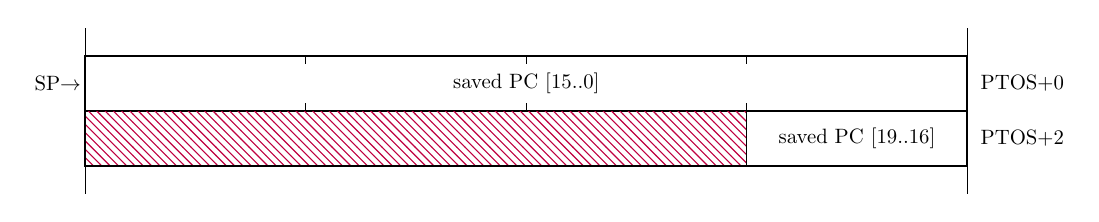
\begin{tikzpicture}[scale=0.7, every node/.style={scale=0.75}]
\draw[thick] (0,3) rectangle ++(16,1); \node at (8,3.5) {saved PC [15..0]};
\foreach \x in {4,8,12} { \draw (\x,3) -- ++(0,.15);  \draw (\x,4) -- ++(0,-.15); }
\draw[thick] (0,2) rectangle ++(16,1); \node at (14,2.5) {saved PC [19..16]};
%\draw[thick] (0,1) rectangle ++(16,1); \node at (8,1.5) {service identifier};
%\foreach \x in {4,8,12} { \draw (\x,1) -- ++(0,.15);  \draw (\x,2) -- ++(0,-.15); }
%\draw[thick] (0,0) rectangle ++(16,1); \node at (14,.5) {saved r11 [19..16]};
%\draw (12,0) -- ++(0,1);
%\draw[pattern=north west lines, pattern color=purple] (0,0) rectangle ++(12,1);
\draw[pattern=north west lines, pattern color=purple] (0,2) rectangle ++(12,1);
\foreach \x in {0,16} \draw (\x,1.5) -- (\x,4.5);
\node at (-.5,3.5) {SP$\rightarrow$};
\foreach \y/\offset in {3.5/0,2.5/2} \node at (17,\y) {PTOS+\offset};
\end{tikzpicture}
\label{fig:stacksc}
\end{figure}

When an interrupt is taken into account, the \lstinline{PC} and the \lstinline{SR} are pushed on the stack. To save space, the \lstinline{SR} is stored in the same 16-bit word as bits 19..16 of \lstinline{PC}. For an obscure reason, words are in reverse order and bits 19..16 of \lstinline{PC} are in high bits. The stack is shown at figure \ref{fig:stackit}.

\begin{figure}[h]
\caption{Stack in an interrupt handler}
\centering
\vspace{1em}
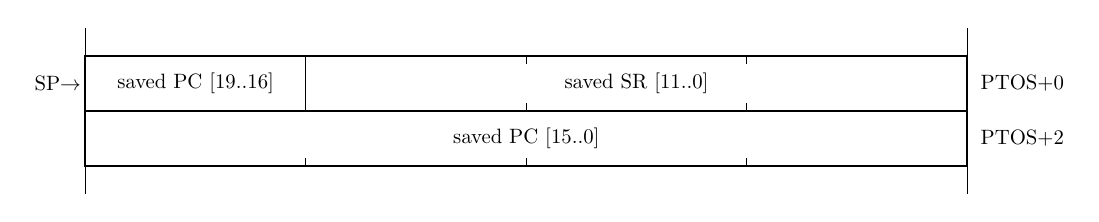
\begin{tikzpicture}[scale=0.7, every node/.style={scale=0.75}]
\draw[thick] (0,2) rectangle ++(16,1); \node at (8,2.5) {saved PC [15..0]};
\foreach \x in {4,8,12} { \draw (\x,2) -- ++(0,.15);  \draw (\x,4) -- ++(0,-.15); }
\draw[thick] (0,3) rectangle ++(16,1); \node at (2,3.5) {saved PC [19..16]}; \node at (10,3.5) {saved SR [11..0]};
\foreach \x in {4,8,12} { \draw (\x,3) -- ++(0,.15);  \draw (\x,4) -- ++(0,-.15); }
%\draw[thick] (0,1) rectangle ++(16,1); \node at (8,1.5) {saved r11 [15..0]};
%\foreach \x in {4,8,12} { \draw (\x,1) -- ++(0,.15);  \draw (\x,2) -- ++(0,-.15); }
%\draw[thick] (0,0) rectangle ++(16,1); \node at (14,.5) {saved r11 [19..16]};
\draw (4,3) -- ++(0,1);
%\draw[pattern=north west lines, pattern color=purple] (0,0) rectangle ++(12,1);
%\draw[pattern=north west lines, pattern color=purple] (0,2) rectangle ++(12,1);
\foreach \x in {0,16} \draw (\x,1.5) -- (\x,4.5);
\node at (-.5,3.5) {SP$\rightarrow$};
\foreach \y/\offset in {3.5/0,2.5/2} \node at (17,\y) {PTOS+\offset};
\end{tikzpicture}
\label{fig:stackit}
\end{figure}

\subsection*{Preemption cases}

A preemption can be synchronous or asynchronous. A synchronous preemption (SP) happens when a service call is done, for instance when a task activates a higher priority task. An asynchronous preemption (AP) happens under interrupt, for instance when a higher priority task is activated by an alarm. A preempted task may resume its execution following a synchronous event (SR) : the running task calls \lstinline{TerminateTask}, \lstinline{ChainTask}, \lstinline{WaitEvent} or \lstinline{SetEvent} or following an asynchronous event (AR) : an alarm does a \lstinline{SetEvent}. So there are 4 cases:.

\begin{description}

\item[SPSR] Synchronous Preemption, Synchronous Resume. $\tau_1$ is running, $\tau_2$ is ready. $P(\tau_1) > P(\tau_2)$.
$\tau_1$ calls \lstinline{WaitEvent} and is preempted synchronously, $\tau_2$ becomes running and  calls \lstinline{SetEvent}. $\tau_2$ is preempted and $\tau_1$ is resumed synchronously.

\item[SPAR] Synchronous Preemption, Asynchronous Resume. $\tau_1$ calls \lstinline{WaitEvent} ans is synchronously preempted, An alarm does a \lstinline{SetEvent} on $\tau_1$ which is asynchronously resumed.

\item[APSR] Asynchronous Preemption, Synchronous Resume. $\tau_1$ is running, $\tau_2$ is suspended. $P(\tau_1) < P(\tau_2)$. An alarm activates $\tau_2$, $\tau_1$ is asynchronously preempted, $\tau_2$ calls \lstinline{TerminateTask}, $\tau_1$ is synchronously resumed.

\item[APAR] Asynchronous Preemption, Asynchronous Resume. $\tau_1$ is running, $\tau_2$ is suspended. $P(\tau_1) < P(\tau_2)$. An alarm activates $\tau_2$, $\tau_1$ is asynchronously preempted. $\tau_2$ is terminated by the OS because of protection fault, for instance a timing protection interrupt and $\tau_1$ is asynchronously resumed.

\end{description}

So \emph{the stack frame has to be normalized}. The normalized stack frame is the asynchronous one shown at figure \ref{fig:stackit} because it contains the Status Register. Normalization is done at the beginning of the \sch. The end of the \sch is done using the \texttt{reti} instruction, as at the end of an interrupt.

The normalized stack frame may be done only when a context is saved to prevent a normalization if there is no context switch. However, the load of the context is much complicated, as the restauration of \texttt{r2} (aka status register) in the \sch re-enable the interrupts before the end of the function.

\section{The tpl\_sc\_handler}

The background color of the code snippets depends on the current active stack:
\begin{description}
	\item[green] process stack
	\item[red]   kernel stack
	\item[yellow] either kernel or process stack
\end{description}

%\fbox{\parbox{.99\textwidth}{The stack structure should be reviewed for the \lstinline{tpl_sc_handler}. Since volatile registers must be stacked first by an ISR, they should be at the bottom of the stack, just above the PC, and not at the top.}}

\vspace{1em}

The first thing to do is to compare the service id to the number of services to verify its validity.

\begin{lstlisting}[backgroundcolor=\color{yellow!15}]
    cmp #SYSCALL_COUNT, REG_SID
    jhs tpl_sc_handler_invalid_service_id
\end{lstlisting}

We need to have the same stack pattern for both the \sch\ and an interrupt handler which calls the operation system. Obviously volatile registers (r12 to r15 because we take into account both ABIs) are not saved in \sch\ since the caller does not expect their values to be preserved but we need to make room (8 bytes) on the stack for them because an interrupt handler will save these registers at this location. The 16 bit words at the bottom of this area is for the \lstinline{REG_RETARG} which is not saved yet.

\begin{lstlisting}[backgroundcolor=\color{yellow!15}]
    sub     #8, r1
\end{lstlisting}

The \sch\ needs one working register and we choose to use \lstinline{r11} which has to be saved on the process stack before using it.

\begin{lstlisting}[backgroundcolor=\color{yellow!15}]
    pushx.w r11
\end{lstlisting}

Then interrupts are disabled.

\begin{lstlisting}[backgroundcolor=\color{yellow!15}]
    dint
\end{lstlisting}

At that stage the stack is as follow:

\begin{center}
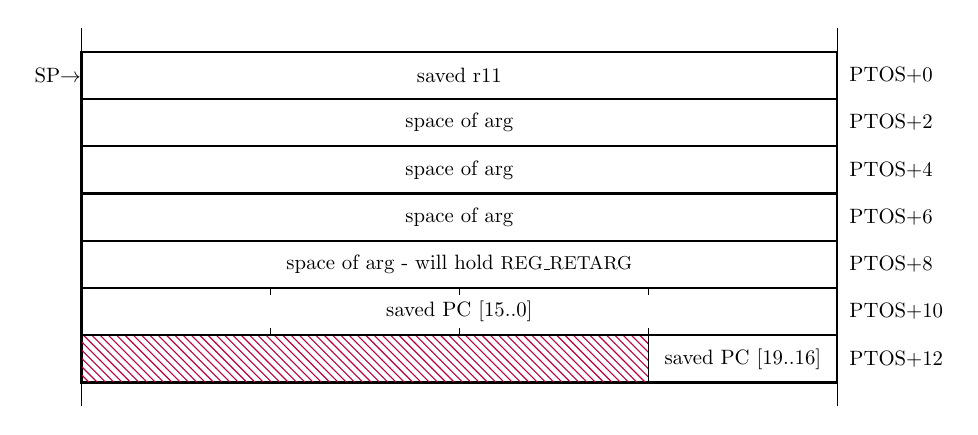
\begin{tikzpicture}[xscale=0.6, yscale=-.6, every node/.style={scale=0.75}]
\draw[thick] (0,0) rectangle ++(16,1); \node at (8,0.5) {saved r11};
\draw[thick] (0,5) rectangle ++(16,1); \node at (8,5.5) {saved PC [15..0]};
%\foreach \x in {4,8,12} { \draw (\x,6) -- ++(0,.15);  \draw (\x,7) -- ++(0,-.15); }
\draw[thick] (0,6) rectangle ++(16,1); \node at (14,6.5) {saved PC [19..16]};% \node at (10,5.5) {saved SR [11..0]};
\draw[pattern=north west lines, pattern color=purple] (0,6) rectangle ++(12,1);
\foreach \x in {4,8,12} { \draw (\x,5) -- ++(0,.15);  \draw (\x,6) -- ++(0,-.15); }
\draw (12,6) -- ++(0,1);
\foreach \y in {1,2,3} {
\draw[thick] (0,\y) rectangle ++(16,1); \node at ($(8,\y+.5)$) {space of arg};
}
\draw[thick] (0,4) rectangle ++(16,1); \node at ($(8,4.5)$) {space of arg - will hold {\small REG\_RETARG}};
\foreach \x in {0,16} \draw (\x,-.5) -- (\x,7.5);
\node at (-.5,0.5) {SP$\rightarrow$};
\foreach \offset in {0,2,...,12} \node[anchor=west] at ($(16.1,.5+.5*\offset)$) {PTOS+\offset};
\end{tikzpicture}
\end{center}



The bottom of the stack have to be updated to the normalized stack (i.e. the stack in an interrupt handler, figure \ref{fig:stackit}).

\begin{lstlisting}[backgroundcolor=\color{yellow!15}]
    mov     12(r1), r11    /* Saved PC [19..16] -> r11                  */
    mov     10(r1), 12(r1) /* Copy saved PC [15..0] at the good place   */
    swpb    r11            /* Get saved PC [19..16] in bits 11..8       */
    rlam.w  #4, r11        /* Shift them to bits 19..16                 */
    bis     r2, r11        /* Add the SR in its location at 11..0       */
    bis     #8, r11        /* set GIE bit (reset just before with dint) */
    mov     r11, 12(r1)    /* The stack is ok                           */
\end{lstlisting}

The stack is then as follow:

\begin{center}
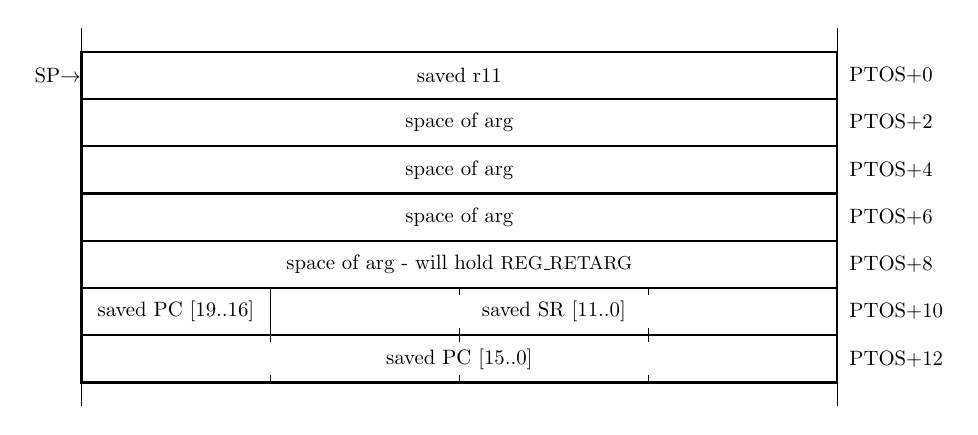
\begin{tikzpicture}[xscale=0.6, yscale=-.6, every node/.style={scale=0.75}]
\draw[thick] (0,0) rectangle ++(16,1); \node at (8,0.5) {saved r11};
\draw[thick] (0,6) rectangle ++(16,1); \node at (8,6.5) {saved PC [15..0]};
\foreach \x in {4,8,12} { \draw (\x,6) -- ++(0,.15);  \draw (\x,7) -- ++(0,-.15); }
\draw[thick] (0,5) rectangle ++(16,1); \node at (2,5.5) {saved PC [19..16]}; \node at (10,5.5) {saved SR [11..0]};
\foreach \x in {8,12} { \draw (\x,5) -- ++(0,.15);  \draw (\x,6) -- ++(0,-.15); }
\draw (4,5) -- ++(0,1);
\foreach \y in {1,2,3} {
\draw[thick] (0,\y) rectangle ++(16,1); \node at ($(8,\y+.5)$) {space of arg};
}
\draw[thick] (0,4) rectangle ++(16,1); \node at ($(8,4.5)$) {space of arg - will hold {\small REG\_RETARG}};
\foreach \x in {0,16} \draw (\x,-.5) -- (\x,7.5);
\node at (-.5,0.5) {SP$\rightarrow$};
\foreach \offset in {0,2,...,12} \node[anchor=west] at ($(16.1,.5+.5*\offset)$) {PTOS+\offset};
\end{tikzpicture}
\end{center}


The reentrancy counter is checked to prevent a switch to the kernel stack when executing a service called by a hook.

\begin{lstlisting}[backgroundcolor=\color{yellow!15}]
    tst.b &tpl_reentrancy_counter
    jnz   tpl_sc_handler_no_stack_switch
\end{lstlisting}

In case of stack switch, the process stack pointer (PSP) is saved on the kernel stack

\begin{lstlisting}[backgroundcolor=\color{red!15}]
    mov  r1,r11
    mov  #tpl_kern_stack_bottom, r1
    push r11
\end{lstlisting}

The kernel stack is as follow (\texttt{KTOS} stands for \emph{Kernel Top Of Stack}):

\begin{center}
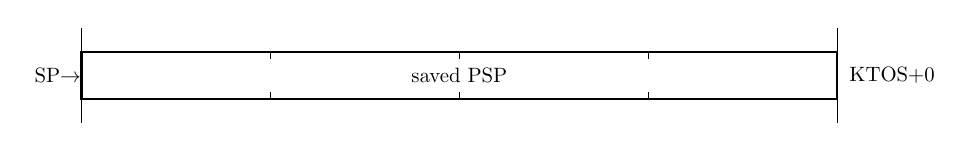
\begin{tikzpicture}[scale=0.6, every node/.style={scale=0.75}]
\draw[thick] (0,3) rectangle ++(16,1); \node at (8,3.5) {saved PSP};
\foreach \x in {4,8,12} { \draw (\x,3) -- ++(0,.15);  \draw (\x,4) -- ++(0,-.15); }
\foreach \x in {0,16} \draw (\x,2.5) -- (\x,4.5);
\node at (-.5,3.5) {SP$\rightarrow$};
\foreach \y/\offset in {3.5/0} \node[anchor=west] at (16.1,\y) {KTOS+\offset};
\end{tikzpicture}
\end{center}

Increment the reentrancy counter.

\begin{lstlisting}[backgroundcolor=\color{red!15}]
tpl_sc_handler_no_stack_switch:
    inc.b &tpl_reentrancy_counter
\end{lstlisting}

Init the \lstinline{NEED_SWITCH}/\lstinline{SAVE} in \lstinline{tpl_kern}.

\begin{lstlisting}[backgroundcolor=\color{red!15}]
    mov #tpl_kern, r11
    mov.b #NO_NEED_SWITCH_NOR_SCHEDULE, TPL_KERN_OFFSET_NEED_SWITCH(r11)
    mov.b #NO_NEED_SWITCH_NOR_SCHEDULE, TPL_KERN_OFFSET_NEED_SCHEDULE(r11)
\end{lstlisting}

Call the service.

\begin{lstlisting}[backgroundcolor=\color{red!15}]
    rla  REG_SID /* index -> offset */
    call tpl_dispatch_table(REG_SID)
\end{lstlisting}

From there, \lstinline{REG_RETARG} holds the return value. It is put at its location in the process stack. Also \lstinline{r13} and \lstinline{r14} become usable whatever is the ABI.

\begin{lstlisting}[backgroundcolor=\color{red!15}]
    pop	    r13 //get back PSP => r13
    movx.w  REG_RETARG, 8(r13) //put in Process's stack
\end{lstlisting}

Check the context switch condition in \lstinline{tpl_kern}.
\begin{lstlisting}[backgroundcolor=\color{red!15}]
    mov     #tpl_kern, r11
    tst.b   TPL_KERN_OFFSET_NEED_SWITCH(r11)
    jz      tpl_sc_handler_no_context_switch
\end{lstlisting}

Prepare the call to \lstinline{tpl_run_elected} by setting \lstinline{REG_RETARG} to 0, aka no save.
\begin{lstlisting}[backgroundcolor=\color{red!15}]
    mov     #0, REG_RETARG
\end{lstlisting}

Test the \lstinline{NEED_SAVE} condition.

\begin{lstlisting}[backgroundcolor=\color{red!15}]
    bit.b   #NEED_SAVE, TPL_KERN_OFFSET_NEED_SWITCH(r11)
    jz      tpl_sc_handler_no_save_running_context
\end{lstlisting}
Save the context. The MSP430 have a ``push multiple words", but no ``move multiple word". So, we get back to process stack to benefit this instruction

\begin{lstlisting}[backgroundcolor=\color{red!15}]
    mov     r1, r14	/* get a copy of the KSP to restore it later */
\end{lstlisting}
\begin{lstlisting}[backgroundcolor=\color{yellow!15}]
    mov     r13, r1	/* change stack to process stack */	
    pushm.w #7, r10	/* Push r4 to r10 on process stack (save) */
\end{lstlisting}
\begin{lstlisting}[backgroundcolor=\color{red!15}]
    mov     r14, r1	/* get back to kernel stack */
\end{lstlisting}

The whole context is now saved on process stack and the kernel stack has been cleaned. The saved context structure is shown at figure \ref{fig:context}.

\begin{figure}[h!]
\caption{Context saved on stack}
\begin{center}
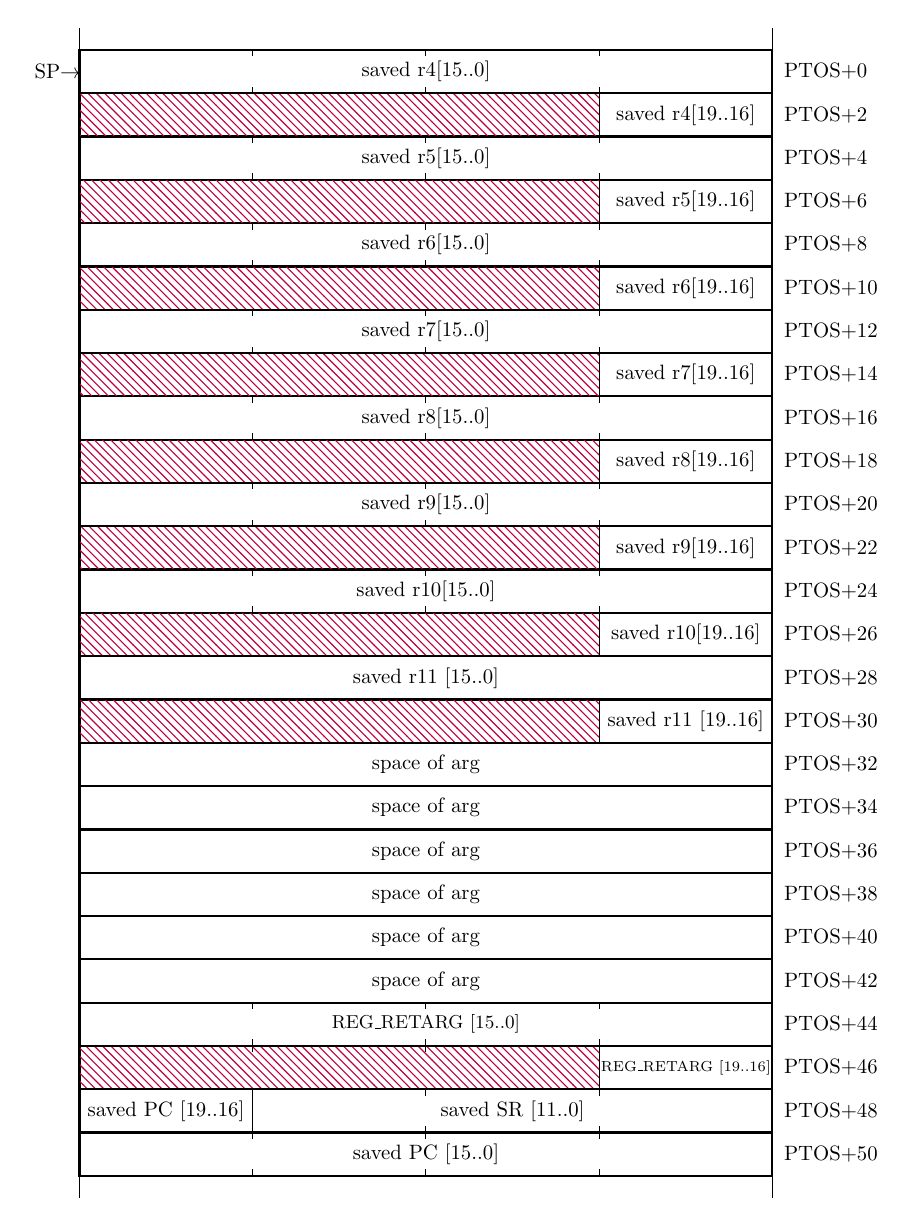
\begin{tikzpicture}[scale=0.55, every node/.style={scale=0.75}]

\foreach \reg/\y in {10/7,9/9,8/11,7/13,6/15,5/17,4/19} {
\draw[thick] ($(0,\y+8)$) rectangle ++(16,1); \node at ($(8,\y+8.5)$) {saved r\reg [15..0]};
\foreach \x in {4,8,12} { \draw ($(\x,\y+8)$) -- ++(0,.15);  \draw ($(\x,\y+9)$) -- ++(0,-.15); }
\draw[thick] ($(0,\y+7)$) rectangle ++(16,1); \node at ($(14,\y+7.5)$) {saved r\reg [19..16]};
\draw[pattern=north west lines, pattern color=purple] ($(0,\y+7)$) rectangle ++(12,1);
}

\draw[thick] (0,5) rectangle ++(16,1); \node at (8,5.5) {\small REG\_RETARG [15..0]};
\foreach \x in {4,8,12} { \draw (\x,23) -- ++(0,.15);  \draw (\x,5) -- ++(0,-.15); }
\draw[thick] (0,4) rectangle ++(16,1); \node at (14,4.5) {\scriptsize REG\_RETARG [19..16]};
\draw[pattern=north west lines, pattern color=purple] (0,4) rectangle ++(12,1);


\foreach \y in {6,7,...,11} {
\draw[thick] (0,\y) rectangle ++(16,1); \node at ($(8,\y+.5)$) {space of arg};
}

\draw[thick] (0,13) rectangle ++(16,1); \node at (8,13.5) {saved r11 [15..0]};
\foreach \x in {4,8,12} { \draw (\x,5) -- ++(0,.15);  \draw (\x,6) -- ++(0,-.15); }
\draw[thick] (0,12) rectangle ++(16,1); \node at (14,12.5) {saved r11 [19..16]};
\draw[pattern=north west lines, pattern color=purple] (0,12) rectangle ++(12,1);

\draw[thick] (0,2) rectangle ++(16,1); \node at (8,2.5) {saved PC [15..0]};
\foreach \x in {4,8,12} { \draw (\x,3) -- ++(0,.15);  \draw (\x,4) -- ++(0,-.15); }
\draw[thick] (0,3) rectangle ++(16,1); \node at (2,3.5) {saved PC [19..16]};
\draw[thick] (0,3) rectangle ++(16,1); \node at (10,3.5) {saved SR [11..0]};
\foreach \x in {4,8,12} { \draw (\x,2) -- ++(0,.15);  \draw (\x,3) -- ++(0,-.15); }
\draw (4,3) -- ++(0,1);
\foreach \x in {0,16} \draw (\x,1.5) -- (\x,28.5);
\node at (-.5,27.5) {SP$\rightarrow$};
\foreach \offset in {0,2,...,50} \node[anchor=west] at ($(16.1,27.5-.5*\offset)$) {PTOS+\offset};
\end{tikzpicture}
\end{center}
\label{fig:context}
\end{figure}

Now the stack pointer is saved in the dedicated location.

\begin{lstlisting}[backgroundcolor=\color{red!15}]
    mov     &tpl_kern, r11  /* Get the s_running slot of tpl_kern in r11 */
    mov     @r11, r11       /* Get the pointer to the context (SP alone) */
    mov     r13, @r11       /* Save the stack pointer                    */
\end{lstlisting}

Prepare the argument of \lstinline{tpl_run_elected} : 1 (aka save) and call it after switching back to the kernel stack.

\begin{lstlisting}[backgroundcolor=\color{red!15}]
    mov     #1, REG_RETARG
tpl_sc_handler_no_save_running_context:
    call    tpl_run_elected
\end{lstlisting}

\lstinline{tpl_run_elected} has copied the elected process slot of \lstinline{tpl_kern} to the \lstinline{running} slot. We load the stack pointer of the new running process.

\begin{lstlisting}[backgroundcolor=\color{red!15}]
    mov &tpl_kern, r11  /* Get the s_running slot of tpl_kern in r11 */
    mov @r11, r11       /* Get the pointer to the context (SP alone) */
\end{lstlisting}
\begin{lstlisting}[backgroundcolor=\color{yellow!15}]
    mov @r11, r1        /* Get the stack pointer                     */
\end{lstlisting}

Now, the context of the new running process is loaded. First we pop \lstinline{r4} to \lstinline{r10}

\begin{lstlisting}[backgroundcolor=\color{yellow!15}]
    popm.a #7,r10       /* Pop r4 to r10  */
	jmp tpl_sc_end_of_context_switch
\end{lstlisting}

The process stack is then as in figure \ref{fig:processStackLoaded}.

\begin{figure}[h!]
\caption{Process stack just loaded}
\begin{center}
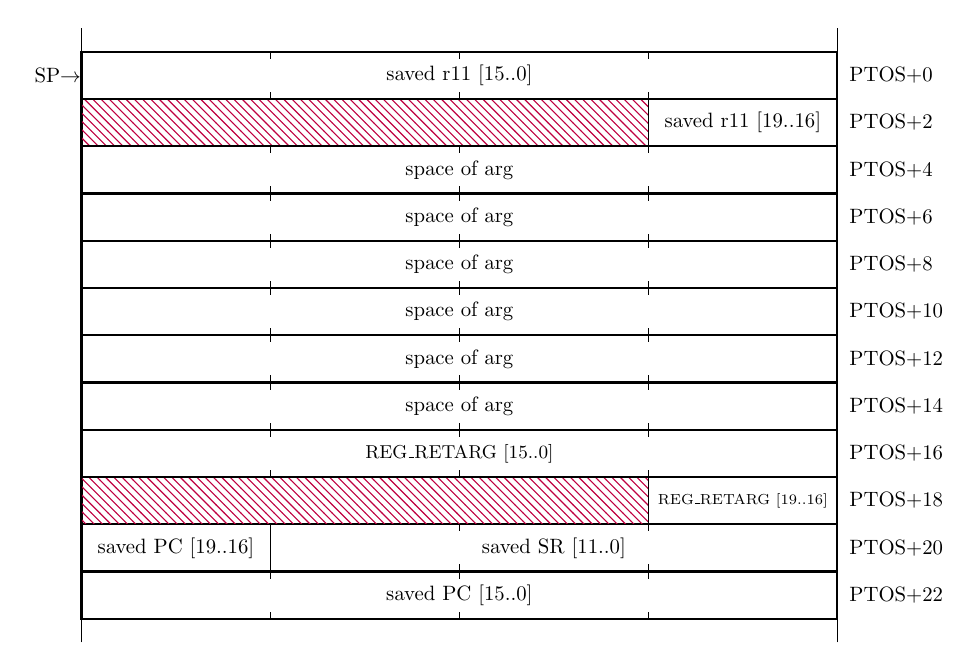
\begin{tikzpicture}[scale=0.6, every node/.style={scale=0.75}]
%\draw[thick] (0,7) rectangle ++(16,1); \node at (8,7.5) {saved r10 [15..0]};
%\foreach \x in {4,8,12} { \draw (\x,7) -- ++(0,.15);  \draw (\x,8) -- ++(0,-.15); }
%\draw[thick] (0,6) rectangle ++(16,1); \node at (14,6.5) {saved r10 [19..16]};
%\draw[pattern=north west lines, pattern color=purple] (0,6) rectangle ++(12,1);
\draw[thick] (0,13) rectangle ++(16,1); \node at (8,13.5) {saved r11 [15..0]};
\foreach \x in {4,8,12} { \draw (\x,13) -- ++(0,.15);  \draw (\x,14) -- ++(0,-.15); }
\draw[thick] (0,12) rectangle ++(16,1); \node at (14,12.5) {saved r11 [19..16]};
\draw[pattern=north west lines, pattern color=purple] (0,12) rectangle ++(12,1);
%\draw[thick] (0,3) rectangle ++(16,1); \node at (8,3.5) {saved PC [15..0]};
%\foreach \x in {4,8,12} { \draw (\x,3) -- ++(0,.15);  \draw (\x,4) -- ++(0,-.15); }
%\draw[thick] (0,2) rectangle ++(16,1); \node at (14,2.5) {saved PC [19..16]};
%\draw[pattern=north west lines, pattern color=purple] (0,2) rectangle ++(12,1);

\draw[thick] (0,2) rectangle ++(16,1); \node at (8,2.5) {saved PC [15..0]};
\foreach \x in {4,8,12} { \draw (\x,3) -- ++(0,.15);  \draw (\x,4) -- ++(0,-.15); }
\draw[thick] (0,3) rectangle ++(16,1); \node at (2,3.5) {saved PC [19..16]};
\draw[thick] (0,3) rectangle ++(16,1); \node at (10,3.5) {saved SR [11..0]};
\foreach \x in {4,8,12} { \draw (\x,2) -- ++(0,.15);  \draw (\x,3) -- ++(0,-.15); }
\draw (4,3) -- ++(0,1);


%\draw[thick] (0,1) rectangle ++(16,1); \node at (8,1.5) {service identifier};
%\foreach \x in {4,8,12} { \draw (\x,1) -- ++(0,.15);  \draw (\x,2) -- ++(0,-.15); }
%\draw[thick] (0,0) rectangle ++(16,1); \node at (14,.5) {saved r11 [19..16]};
%\draw (12,0) -- ++(0,1);
%\draw[pattern=north west lines, pattern color=purple] (0,0) rectangle ++(12,1);

\foreach \y in {6,7,...,11} {
\draw[thick] (0,\y) rectangle ++(16,1); \node at ($(8,\y+.5)$) {space of arg};
\foreach \x in {4,8,12} { \draw (\x,\y) -- ++(0,.15);  \draw ($(\x,\y+1)$) -- ++(0,-.15); }
}

\draw[thick] (0,5) rectangle ++(16,1); \node at ($(8,5.5)$) {\small REG\_RETARG [15..0]};
\foreach \x in {4,8,12} { \draw (\x,5) -- ++(0,.15);  \draw ($(\x,6)$) -- ++(0,-.15); }
\draw[thick] (0,4) rectangle ++(16,1); \node at ($(14,4.5)$) {\scriptsize REG\_RETARG [19..16]};
\draw[pattern=north west lines, pattern color=purple] (0,4) rectangle ++(12,1);

\foreach \x in {0,16} \draw (\x,1.5) -- (\x,14.5);
\node at (-.5,13.5) {SP$\rightarrow$};
\foreach \offset in {0,2,...,22} \node[anchor=west] at ($(16.1,13.5-.5*\offset)$) {PTOS+\offset};
\end{tikzpicture}
\end{center}
\label{fig:processStackLoaded}
\end{figure}

In case of no context switch, we have to get to the process stack, stored in r13

\begin{lstlisting}[backgroundcolor=\color{red!15}]
tpl_sc_handler_no_context_switch:
	mov r13, r1	 /* get back to process stack */
\end{lstlisting}
At last the reentrancy counter is decremented, r11 is restored, the \emph{space of args}, used in asynchronous preemption is removed from stack and the \lstinline{REG_RETARG} is poped.

Interrupts are enables during the \texttt{reti} instruction because it is related to the \texttt{GIE} bit in the status register.
\begin{lstlisting}[backgroundcolor=\color{yellow!15}]
tpl_sc_end_of_context_switch:
    dec.b  &tpl_reentrancy_counter
    jnz    tpl_sc_handler_still_in_kernel    

tpl_sc_handler_still_in_kernel:
    popx.a r11
    add    #12,r1       /* Skip volatile             */
    popx.a REG_RETARG   /* Get back the return value */
    reti
\end{lstlisting}

\subsection{Context initialisation}
The context that shoud be set during the task's initialisation (\texttt{tpl\_init\_context}) is the one of the figure \ref{fig:context}, but with a call to either \texttt{CallTerminateTask} or \texttt{CallTerminateISR2}, depending of the type of the process to init.

\emph{TODO} Works only with 16-bit register.Should be updated.

\begin{figure}[h!]
\caption{Context initialisation}
\begin{center}
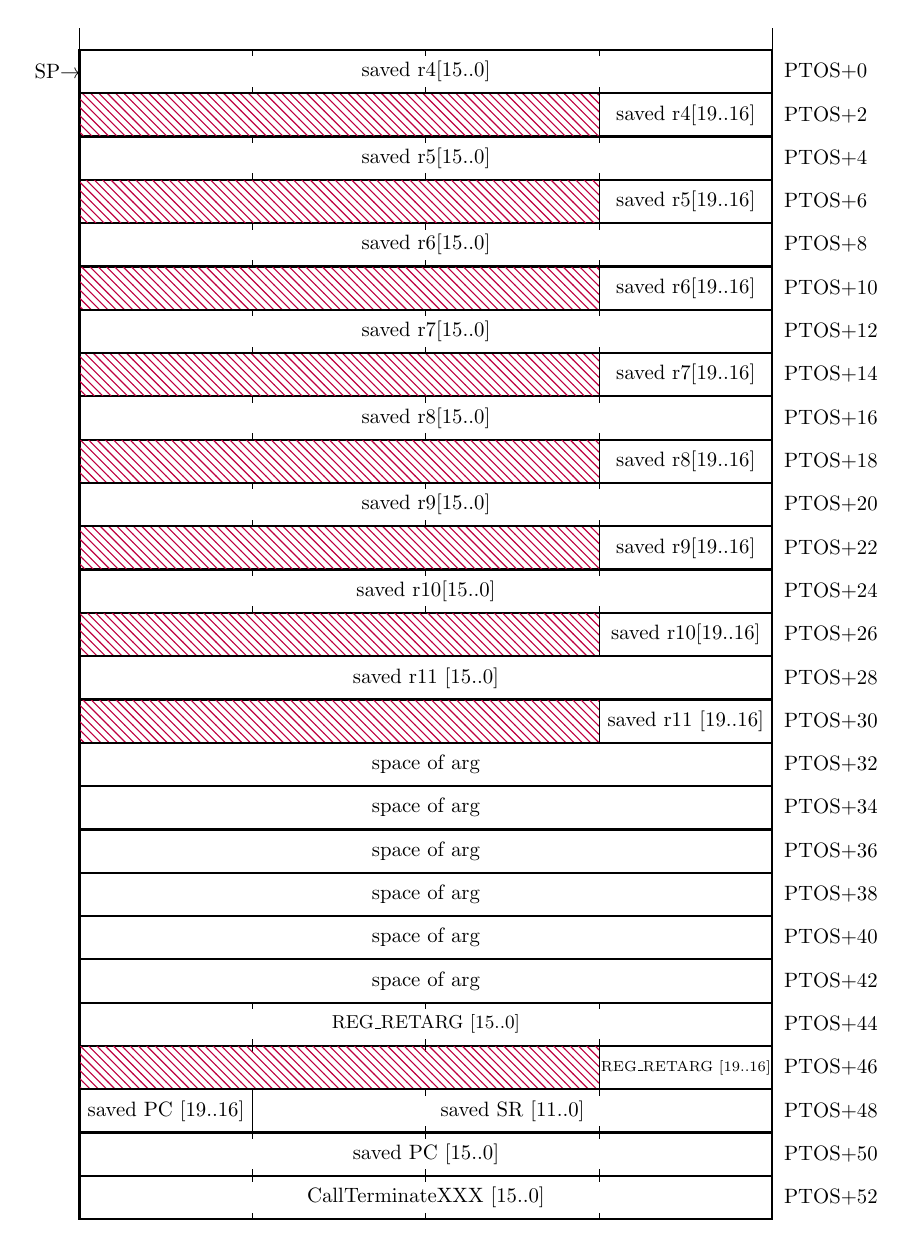
\begin{tikzpicture}[scale=0.55, every node/.style={scale=0.75}]

\foreach \reg/\y in {10/7,9/9,8/11,7/13,6/15,5/17,4/19} {
\draw[thick] ($(0,\y+8)$) rectangle ++(16,1); \node at ($(8,\y+8.5)$) {saved r\reg [15..0]};
\foreach \x in {4,8,12} { \draw ($(\x,\y+8)$) -- ++(0,.15);  \draw ($(\x,\y+9)$) -- ++(0,-.15); }
\draw[thick] ($(0,\y+7)$) rectangle ++(16,1); \node at ($(14,\y+7.5)$) {saved r\reg [19..16]};
\draw[pattern=north west lines, pattern color=purple] ($(0,\y+7)$) rectangle ++(12,1);
}

\draw[thick] (0,5) rectangle ++(16,1); \node at (8,5.5) {\small REG\_RETARG [15..0]};
\foreach \x in {4,8,12} { \draw (\x,23) -- ++(0,.15);  \draw (\x,5) -- ++(0,-.15); }
\draw[thick] (0,4) rectangle ++(16,1); \node at (14,4.5) {\scriptsize REG\_RETARG [19..16]};
\draw[pattern=north west lines, pattern color=purple] (0,4) rectangle ++(12,1);


\foreach \y in {6,7,...,11} {
\draw[thick] (0,\y) rectangle ++(16,1); \node at ($(8,\y+.5)$) {space of arg};
}

%\draw[thick] (0,6) rectangle ++(16,1); \node at (8,6.5) {saved r15};
%\foreach \x in {4,8,12} { \draw (\x,6) -- ++(0,.15);  \draw (\x,7) -- ++(0,-.15); }

\draw[thick] (0,13) rectangle ++(16,1); \node at (8,13.5) {saved r11 [15..0]};
\foreach \x in {4,8,12} { \draw (\x,5) -- ++(0,.15);  \draw (\x,6) -- ++(0,-.15); }
\draw[thick] (0,12) rectangle ++(16,1); \node at (14,12.5) {saved r11 [19..16]};
\draw[pattern=north west lines, pattern color=purple] (0,12) rectangle ++(12,1);

\draw[thick] (0,2) rectangle ++(16,1); \node at (8,2.5) {saved PC [15..0]};
\foreach \x in {4,8,12} { \draw (\x,3) -- ++(0,.15);  \draw (\x,4) -- ++(0,-.15); }
\draw[thick] (0,3) rectangle ++(16,1); \node at (2,3.5) {saved PC [19..16]};
\draw[thick] (0,3) rectangle ++(16,1); \node at (10,3.5) {saved SR [11..0]};
\foreach \x in {4,8,12} { \draw (\x,2) -- ++(0,.15);  \draw (\x,3) -- ++(0,-.15); }
\draw (4,3) -- ++(0,1);
\foreach \x in {0,16} \draw (\x,1.5) -- (\x,28.5);
\node at (-.5,27.5) {SP$\rightarrow$};
\foreach \offset in {0,2,...,52} \node[anchor=west] at ($(16.1,27.5-.5*\offset)$) {PTOS+\offset};
%22.5/0,21.5/2,20.5/4,19.5/6,18.5/8,17.5/10,16.5/12,15.5/14,14.5/16,13.5/18,
%12.5/20,11.5/22,10.5/24,9.5/26,8.5/28,7.5/30,6.5/32,5.5/34,4.5/36,3.5/38,2.5/40,
%1.5/42,0.5/44,-.5/46,-1.5/48,-2.5/50,-3.5/52,-4.5/54
%} \node[anchor=west] at ($(16.1,\y+7)$) {PTOS+\offset};
\draw[thick] (0,1) rectangle ++(16,1); \node at (8,1.5) {CallTerminateXXX [15..0]};
\foreach \x in {4,8,12} { \draw (\x,1) -- ++(0,.15);  \draw (\x,2) -- ++(0,-.15); }
\end{tikzpicture}
\end{center}
\label{fig:context}
\end{figure}


\section{The Systick Handler}

The Systick is generated by using a \lstinline{TIMERA} register. On the MSP430FR5969, \lstinline{TIMERA3} has been chosen. When entering the ISR, the stack is as shown at figure \ref{fig:stackit} and \lstinline{PC} (\lstinline{r0}) and \lstinline{SR} (\lstinline{r2}) have been saved. Before doing anything we have to save the volatile registers, which are \lstinline{r11}\footnote{r11 is not volatile in the \emph{MSPGCC} ABI but is volatile in \emph{GCC compiler for MSP} ABI. Anyway, in order to limit variabilility, \lstinline{r11} is saved for both ABIs.} to \lstinline{r15}, because they will not be saved when we will call the \lstinline{tpl_counter_tick_SystemCounter} C function.

\begin{lstlisting}[basicstyle=\footnotesize\ttfamily]
tpl_systick_handler:
    pushx.a REG_RETARG
#ifdef MSPGCC_ABI
    /* r15 has been pushed by pushx.a REG_RETARG */
    pushm.a #4, r14  /* Push r11, r12, r13, r14 */
#endif
#ifdef GCCFORMSP_ABI
    /* r12 has been pushed by pushx.a REG_RETARG */
    pushm.a #3, r15  /* Push r13, r14, r15 */
    pushx.a r11
#endif
\end{lstlisting}

As a result the stack is as follow for \emph{MSPGCC} ABI:

\begin{center}
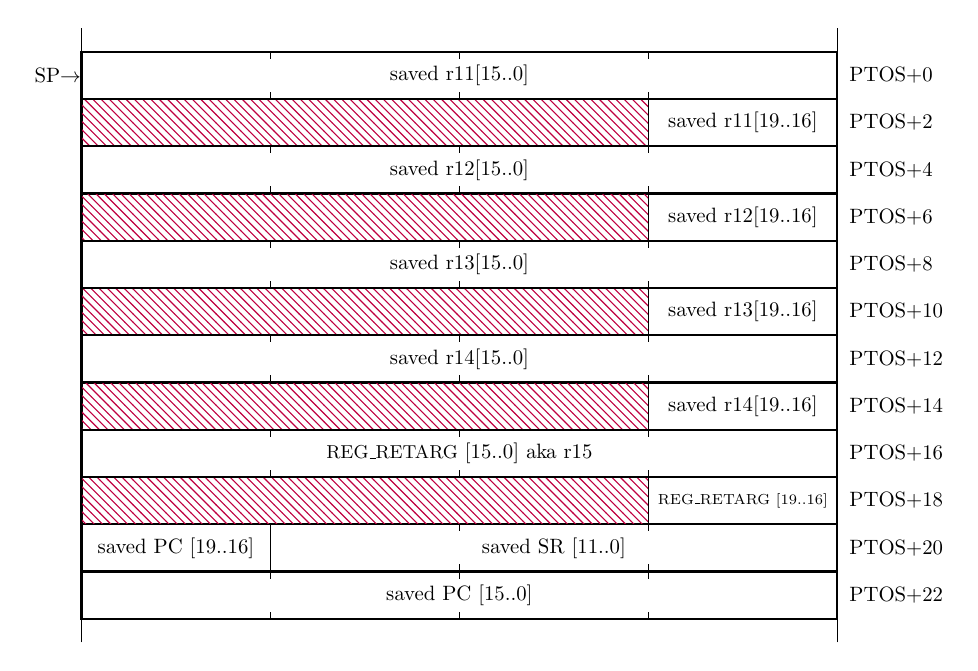
\begin{tikzpicture}[scale=0.6, every node/.style={scale=0.75}]
%\draw[thick] (0,7) rectangle ++(16,1); \node at (8,7.5) {saved r10 [15..0]};
%\foreach \x in {4,8,12} { \draw (\x,7) -- ++(0,.15);  \draw (\x,8) -- ++(0,-.15); }
%\draw[thick] (0,6) rectangle ++(16,1); \node at (14,6.5) {saved r10 [19..16]};
%\draw[pattern=north west lines, pattern color=purple] (0,6) rectangle ++(12,1);
%\draw[thick] (0,13) rectangle ++(16,1); \node at (8,13.5) {saved r11 [15..0]};
%\foreach \x in {4,8,12} { \draw (\x,13) -- ++(0,.15);  \draw (\x,14) -- ++(0,-.15); }
%\draw[thick] (0,12) rectangle ++(16,1); \node at (14,12.5) {saved r11 [19..16]};
%\draw[pattern=north west lines, pattern color=purple] (0,12) rectangle ++(12,1);
%\draw[thick] (0,3) rectangle ++(16,1); \node at (8,3.5) {saved PC [15..0]};
%\foreach \x in {4,8,12} { \draw (\x,3) -- ++(0,.15);  \draw (\x,4) -- ++(0,-.15); }
%\draw[thick] (0,2) rectangle ++(16,1); \node at (14,2.5) {saved PC [19..16]};
%\draw[pattern=north west lines, pattern color=purple] (0,2) rectangle ++(12,1);

\draw[thick] (0,2) rectangle ++(16,1); \node at (8,2.5) {saved PC [15..0]};
\foreach \x in {4,8,12} { \draw (\x,3) -- ++(0,.15);  \draw (\x,4) -- ++(0,-.15); }
\draw[thick] (0,3) rectangle ++(16,1); \node at (2,3.5) {saved PC [19..16]};
\draw[thick] (0,3) rectangle ++(16,1); \node at (10,3.5) {saved SR [11..0]};
\foreach \x in {4,8,12} { \draw (\x,2) -- ++(0,.15);  \draw (\x,3) -- ++(0,-.15); }
\draw (4,3) -- ++(0,1);


%\draw[thick] (0,1) rectangle ++(16,1); \node at (8,1.5) {service identifier};
%\foreach \x in {4,8,12} { \draw (\x,1) -- ++(0,.15);  \draw (\x,2) -- ++(0,-.15); }
%\draw[thick] (0,0) rectangle ++(16,1); \node at (14,.5) {saved r11 [19..16]};
%\draw (12,0) -- ++(0,1);
%\draw[pattern=north west lines, pattern color=purple] (0,0) rectangle ++(12,1);

%\foreach \y in {6,7,...,11} {
%\draw[thick] (0,\y) rectangle ++(16,1); \node at ($(8,\y+.5)$) {space of arg};
%\foreach \x in {4,8,12} { \draw (\x,\y) -- ++(0,.15);  \draw ($(\x,\y+1)$) -- ++(0,-.15); }
%}
\foreach \reg in {11,12,13,14} {
\draw[thick] ($(0,35-2*\reg)$) rectangle ++(16,1); \node at ($(8,35.5-2*\reg)$) {saved r\reg [15..0]};
\foreach \x in {4,8,12} { \draw ($(\x,35-2*\reg)$) -- ++(0,.15);  \draw ($(\x,36-2*\reg)$) -- ++(0,-.15); }
\draw[thick] ($(0,34-2*\reg)$) rectangle ++(16,1); \node at ($(14,34.5-2*\reg)$) {saved r\reg [19..16]};
\draw[pattern=north west lines, pattern color=purple] ($(0,34-2*\reg)$) rectangle ++(12,1);
}

\draw[thick] (0,5) rectangle ++(16,1); \node at ($(8,5.5)$) {{\small REG\_RETARG} [15..0] aka r15};
\foreach \x in {4,8,12} { \draw (\x,5) -- ++(0,.15);  \draw ($(\x,6)$) -- ++(0,-.15); }
\draw[thick] (0,4) rectangle ++(16,1); \node at ($(14,4.5)$) {\scriptsize REG\_RETARG [19..16]};
\draw[pattern=north west lines, pattern color=purple] (0,4) rectangle ++(12,1);

\foreach \x in {0,16} \draw (\x,1.5) -- (\x,14.5);
\node at (-.5,13.5) {SP$\rightarrow$};
\foreach \offset in {0,2,...,22} \node[anchor=west] at ($(16.1,13.5-.5*\offset)$) {PTOS+\offset};
\end{tikzpicture}
\end{center}
%\begin{center}
%\begin{tikzpicture}[scale=0.7, every node/.style={scale=0.75}]
%
%%\foreach \reg/\y in {15/} {
%%\draw[thick] (0,5) rectangle ++(16,1); \node at (8,5.5) {saved r11 [15..0]};
%%\foreach \x in {4,8,12} { \draw (\x,5) -- ++(0,.15);  \draw (\x,6) -- ++(0,-.15); }
%%\draw[thick] (0,4) rectangle ++(16,1); \node at (14,4.5) {saved r11 [19..16]};
%%\draw[pattern=north west lines, pattern color=purple] (0,4) rectangle ++(12,1);
%%}
%
%\draw[thick] (0,2) rectangle ++(16,1); \node at (8,2.5) {saved PC [15..0]};
%\foreach \x in {4,8,12} { \draw (\x,3) -- ++(0,.15);  \draw (\x,4) -- ++(0,-.15); }
%\draw[thick] (0,3) rectangle ++(16,1); \node at (2,3.5) {saved PC [19..16]};
%\draw[thick] (0,3) rectangle ++(16,1); \node at (10,3.5) {saved SR [11..0]};
%\foreach \x in {4,8,12} { \draw (\x,2) -- ++(0,.15);  \draw (\x,3) -- ++(0,-.15); }
%\draw (4,3) -- ++(0,1);
%\foreach \x in {0,16} \draw (\x,1.5) -- (\x,6.5);
%\node at (-.5,5.5) {SP$\rightarrow$};
%\foreach \y/\offset in {5.5/0,4.5/2,3.5/4,2.5/6} \node at (17,\y) {PTOS+\offset};
%\end{tikzpicture}
%\end{center}

And as follow for the \emph{GCC compiler for MSP} ABI:

\begin{center}
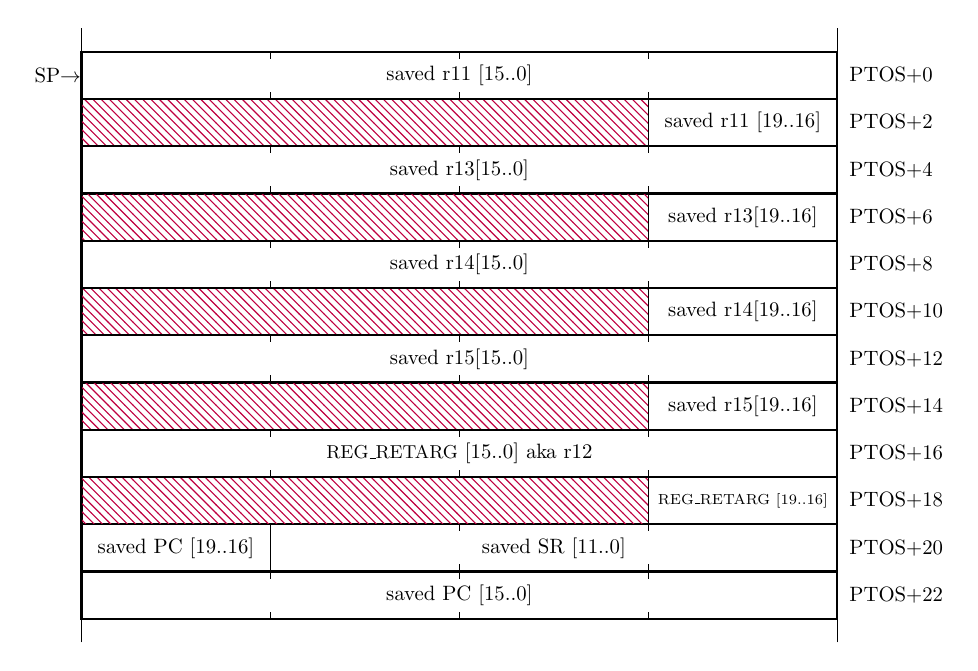
\begin{tikzpicture}[scale=0.6, every node/.style={scale=0.75}]
%\draw[thick] (0,7) rectangle ++(16,1); \node at (8,7.5) {saved r10 [15..0]};
%\foreach \x in {4,8,12} { \draw (\x,7) -- ++(0,.15);  \draw (\x,8) -- ++(0,-.15); }
%\draw[thick] (0,6) rectangle ++(16,1); \node at (14,6.5) {saved r10 [19..16]};
%\draw[pattern=north west lines, pattern color=purple] (0,6) rectangle ++(12,1);
\draw[thick] (0,13) rectangle ++(16,1); \node at (8,13.5) {saved r11 [15..0]};
\foreach \x in {4,8,12} { \draw (\x,13) -- ++(0,.15);  \draw (\x,14) -- ++(0,-.15); }
\draw[thick] (0,12) rectangle ++(16,1); \node at (14,12.5) {saved r11 [19..16]};
\draw[pattern=north west lines, pattern color=purple] (0,12) rectangle ++(12,1);
%\draw[thick] (0,3) rectangle ++(16,1); \node at (8,3.5) {saved PC [15..0]};
%\foreach \x in {4,8,12} { \draw (\x,3) -- ++(0,.15);  \draw (\x,4) -- ++(0,-.15); }
%\draw[thick] (0,2) rectangle ++(16,1); \node at (14,2.5) {saved PC [19..16]};
%\draw[pattern=north west lines, pattern color=purple] (0,2) rectangle ++(12,1);

\draw[thick] (0,2) rectangle ++(16,1); \node at (8,2.5) {saved PC [15..0]};
\foreach \x in {4,8,12} { \draw (\x,3) -- ++(0,.15);  \draw (\x,4) -- ++(0,-.15); }
\draw[thick] (0,3) rectangle ++(16,1); \node at (2,3.5) {saved PC [19..16]};
\draw[thick] (0,3) rectangle ++(16,1); \node at (10,3.5) {saved SR [11..0]};
\foreach \x in {4,8,12} { \draw (\x,2) -- ++(0,.15);  \draw (\x,3) -- ++(0,-.15); }
\draw (4,3) -- ++(0,1);


%\draw[thick] (0,1) rectangle ++(16,1); \node at (8,1.5) {service identifier};
%\foreach \x in {4,8,12} { \draw (\x,1) -- ++(0,.15);  \draw (\x,2) -- ++(0,-.15); }
%\draw[thick] (0,0) rectangle ++(16,1); \node at (14,.5) {saved r11 [19..16]};
%\draw (12,0) -- ++(0,1);
%\draw[pattern=north west lines, pattern color=purple] (0,0) rectangle ++(12,1);

%\foreach \y in {6,7,...,11} {
%\draw[thick] (0,\y) rectangle ++(16,1); \node at ($(8,\y+.5)$) {space of arg};
%\foreach \x in {4,8,12} { \draw (\x,\y) -- ++(0,.15);  \draw ($(\x,\y+1)$) -- ++(0,-.15); }
%}
\foreach \reg in {13,14,15} {
\draw[thick] ($(0,37-2*\reg)$) rectangle ++(16,1); \node at ($(8,37.5-2*\reg)$) {saved r\reg [15..0]};
\foreach \x in {4,8,12} { \draw ($(\x,37-2*\reg)$) -- ++(0,.15);  \draw ($(\x,38-2*\reg)$) -- ++(0,-.15); }
\draw[thick] ($(0,36-2*\reg)$) rectangle ++(16,1); \node at ($(14,36.5-2*\reg)$) {saved r\reg [19..16]};
\draw[pattern=north west lines, pattern color=purple] ($(0,36-2*\reg)$) rectangle ++(12,1);
}

\draw[thick] (0,5) rectangle ++(16,1); \node at ($(8,5.5)$) {{\small REG\_RETARG} [15..0] aka r12};
\foreach \x in {4,8,12} { \draw (\x,5) -- ++(0,.15);  \draw ($(\x,6)$) -- ++(0,-.15); }
\draw[thick] (0,4) rectangle ++(16,1); \node at ($(14,4.5)$) {\scriptsize REG\_RETARG [19..16]};
\draw[pattern=north west lines, pattern color=purple] (0,4) rectangle ++(12,1);

\foreach \x in {0,16} \draw (\x,1.5) -- (\x,14.5);
\node at (-.5,13.5) {SP$\rightarrow$};
\foreach \offset in {0,2,...,22} \node[anchor=west] at ($(16.1,13.5-.5*\offset)$) {PTOS+\offset};
\end{tikzpicture}
\end{center}

Switch to the kernel stack.

\begin{lstlisting}[basicstyle=\footnotesize\ttfamily]
    mov r1,r11                     /* Copy the PSP in r11        */
    mov #tpl_kern_stack_bottom, r1 /* Switch to the kernel stack */
    push r11                       /* Save PCP to kernel stack   */
\end{lstlisting}

The kernel stack is as follow:

\begin{center}
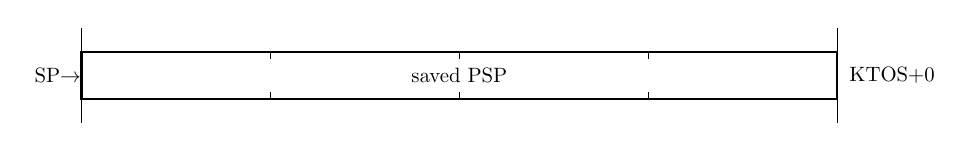
\begin{tikzpicture}[scale=0.6, every node/.style={scale=0.75}]
%\draw[thick] (0,7) rectangle ++(16,1); \node at (8,7.5) {saved r10 [15..0]};
%\foreach \x in {4,8,12} { \draw (\x,7) -- ++(0,.15);  \draw (\x,8) -- ++(0,-.15); }
%\draw[thick] (0,6) rectangle ++(16,1); \node at (14,6.5) {saved r10 [19..16]};
%\draw[pattern=north west lines, pattern color=purple] (0,6) rectangle ++(12,1);
%\draw[thick] (0,5) rectangle ++(16,1); \node at (8,5.5) {saved r11 [15..0]};
%\foreach \x in {4,8,12} { \draw (\x,5) -- ++(0,.15);  \draw (\x,6) -- ++(0,-.15); }
%\draw[thick] (0,4) rectangle ++(16,1); \node at (14,4.5) {saved r11 [19..16]};
%\draw[pattern=north west lines, pattern color=purple] (0,4) rectangle ++(12,1);
\draw[thick] (0,3) rectangle ++(16,1); \node at (8,3.5) {saved PSP};
\foreach \x in {4,8,12} { \draw (\x,3) -- ++(0,.15);  \draw (\x,4) -- ++(0,-.15); }
%\draw[thick] (0,2) rectangle ++(16,1); \node at (14,2.5) {saved PC [19..16]};
%\draw[pattern=north west lines, pattern color=purple] (0,2) rectangle ++(12,1);
%\draw[thick] (0,1) rectangle ++(16,1); \node at (8,1.5) {service identifier};
%\foreach \x in {4,8,12} { \draw (\x,1) -- ++(0,.15);  \draw (\x,2) -- ++(0,-.15); }
%\draw[thick] (0,0) rectangle ++(16,1); \node at (14,.5) {saved r11 [19..16]};
%\draw (12,0) -- ++(0,1);
%\draw[pattern=north west lines, pattern color=purple] (0,0) rectangle ++(12,1);
\foreach \x in {0,16} \draw (\x,2.5) -- (\x,4.5);
\node at (-.5,3.5) {SP$\rightarrow$};
\foreach \y/\offset in {3.5/0} \node[anchor=west] at (16.1,\y) {KTOS+\offset};
\end{tikzpicture}
\end{center}

Init the \lstinline{NEED_SWITCH}/\lstinline{SAVE} in \lstinline{tpl_kern}.

\begin{lstlisting}[basicstyle=\footnotesize\ttfamily]
    mov   #tpl_kern, r11
    mov.b #NO_NEED_SWITCH_NOR_SCHEDULE, TPL_KERN_OFFSET_NEED_SWITCH(r11)
    mov.b #NO_NEED_SWITCH_NOR_SCHEDULE, TPL_KERN_OFFSET_NEED_SCHEDULE(r11)
\end{lstlisting}

Call the function that increments the SystemCounter and manages alarm.

\begin{lstlisting}[basicstyle=\footnotesize\ttfamily]
    call tpl_counter_tick_SystemCounter
\end{lstlisting}

Switch back to the process stack

\begin{lstlisting}[basicstyle=\footnotesize\ttfamily]
    mov r1, r13 /* get a copy of the KSP to restore it later */
    pop r1      /* get the saved process stack pointer back  */
\end{lstlisting}

Check the context switch condition in \lstinline{tpl_kern}.

\begin{lstlisting}[basicstyle=\footnotesize\ttfamily]
    mov   #tpl_kern, r11
    tst.b TPL_KERN_OFFSET_NEED_SWITCH(r11)
    jz    tpl_systick_handler_no_context_switch
\end{lstlisting}

Save the rest of the context.

\begin{lstlisting}[basicstyle=\footnotesize\ttfamily]
    pushm.a #7, r10 /* Push r4 to r10 */
\end{lstlisting}

Now the stack pointer is saved in the dedicated location.

\begin{lstlisting}[basicstyle=\footnotesize\ttfamily]
    mov &tpl_kern, r11  /* Get the s_running slot of tpl_kern in r11 */
    mov @r11, r11       /* Get the pointer to the context (SP alone) */
    mov r1, @r11        /* Save the stack pointer                    */
\end{lstlisting}

Call \lstinline{tpl_run_elected} with argument 1 (aka save) after switching back to the kernel stack.

\begin{lstlisting}[basicstyle=\footnotesize\ttfamily]
    mov r13, r1         /* Switch back to the kernel stack         */
    mov #1, REG_RETARG
    add #2, r1          /* "pop" the PSP which is no longer useful */
    call tpl_run_elected
\end{lstlisting}

\lstinline{tpl_run_elected} has copied the elected process slot of \lstinline{tpl_kern} to the \lstinline{running} slot. We load the stack pointer of the new running process.

\begin{lstlisting}[basicstyle=\footnotesize\ttfamily]
    mov &tpl_kern, r11  /* Get the s_running slot of tpl_kern in r11 */
    mov @r11, r11       /* Get the pointer to the context (SP alone) */
    mov @r11, r1        /* Get the stack pointer                     */
\end{lstlisting}

Now, the context of the new running process is loaded. First we pop \lstinline{r4} to \lstinline{r10}

\begin{lstlisting}[basicstyle=\footnotesize\ttfamily]
    popm.a #7,r10       /* Pop r4 to r10  */
\end{lstlisting}



Restore the volatile registers and return from the interrupt handler.

\begin{lstlisting}[basicstyle=\footnotesize\ttfamily]
tpl_systick_handler_no_context_switch:

#ifdef MSPGCC_ABI
    /* r15 will be popped by popx.a REG_RETARG */
    popm.a #4, r14  /* Pop r11, r12, r13, r14 */
#endif
#ifdef GCCFORMSP_ABI
    /* r12 will be popped by popx.a REG_RETARG */
    popx.a r11
    popm.a #3, r15  /* Pop r13, r14, r15 */
#endif
    popx.a REG_RETARG
    reti
\end{lstlisting}

That's all !

\bibliographystyle{plain}
\bibliography{porting}

\end{document}  

%!TEX root = ./trampoline.tex

\chapter{Ports details}

\section{PowerPC}

\subsection{The MPC5510 Memory Protection Unit}

The access control rights of the memory region descriptor rules the access of 5 bus masters (labeled from 4 to 0). Unused bus masters are set to the same access right for all the regions. Bus master 4 is used for factory testing only, so the access rights should be set to no access. Bus master 3 is the Flexray controller. Since it is not used in the current version of Trampoline, it is set to no access to. Bus master 2 is the DMA controller. For the same reason it is set to no access. Bus master 1 is the Z0 core. Again it is set to no access.

The access control rights register has the following bit usage:

\includegraphics[width=\textwidth]{pictures/MPUacr.pdf} 

Bus master 4 is a special case. The 2 bits have the following meaning:

\rowcolors{1}{white}{light-gray}
\begin{longtableii}{p{0.4in}|p{4.8in}}{}{Bit}{Meaning}
  \lineii{M4RE}
  {If set to 1, bus master 4 may \strong{read} memory in the region. If 0, no read is allowed}
  \lineii{M4WE}
  {If set to 1, bus master 4 may \strong{write} memory in the region. If 0, no write is allowed}
\end{longtableii}

So in our case, these bits are set to 0.

Of course, other bus masters have more sophisticated access right:

\rowcolors{1}{white}{light-gray}
\begin{longtableii}{p{0.4in}|p{4.8in}}{}{Bit}{Meaning}
  \lineii{MxPE}
  {The PID Enable bit. Set to 0 in our case}
  \lineii{MxSM}
  {These 2 bits rules the supervisor mode access control with the following meaning: $00=rwx$, $01=rx$, $10=rw$, $11=$ {\it same as defined by MxUM}. In our case, it is set to $00$ for code and constants and to $11$ for data.}
  \lineii{MxUM}
  {These 2 bits rules the user mode access control. The first bit means $r$, the second one $w$ and the third one $x$.}
\end{longtableii}

Trampoline uses 4 descriptors:

\rowcolors{1}{white}{light-gray}
\begin{longtableiii}{p{0.8in}|p{2in}|p{2.3in}}{}{Descriptor}{Usage}{MxUM value}
  \lineiii{MPU\_RGD0}
  {Constants and program\footnote{This region is set to the whole addressing space. This is not definitive and should be improved because reading a peripheral control register should be protected. So an additional descriptor has to be used to allow the kernel (supervisor mode) a complete access on all the memory space and no access at all for applications (user mode).}.}
  {$rwx=00$ for supervisor mode, $rx=101$ for user mode.}
  \lineiii{MPU\_RGD1}
  {Private variables of the process.}
  {$rw=110$ for supervisor and user mode.}
  \lineiii{MPU\_RGD2}
  {Stack of the process.}
  {$rw=110$ for supervisor and user mode.}
  \lineiii{MPU\_RGD3}
  {Variables of the OS Application if OS Applications are used.}
  {$rw=110$ for supervisor and user mode.}
\end{longtableiii}

So values of access control bits should be:

\includegraphics[width=\textwidth]{pictures/MPUprog.pdf} 

So in hexa:

\rowcolors{1}{white}{light-gray}
\begin{longtableii}{l|l}{}{Kind}{Value}
  \lineii{Program region access}
  {$0x00000005$}
  \lineii{Variable region access}
  {$0x0000001E$}
\end{longtableii}

\subsubsection{What happen in case of memory protection violation ?}

Two exception handler are used to handle a memory protection violation, one for data access, one for code access.

The Data Storage exception is tied to the IVOR~2 vector (VPR offset = 0x020), see page 8-2 of the {\em MPC5510 Microcontroller Family Reference Manual}.

The Instruction Storage exception is tied to the IVOR~3 vector (VPR offset = 0x030), see page 8-2 of the {\em MPC5510 Microcontroller Family Reference Manual}.

However, it appears one of these exceptions is raised when the processor is in user mode. The behavior is different in supervisor mode {\em to be completed}.



\part{The Goil system generator}
%!TEX root = ./main.tex

\chapter{The Goil templates}
\label{chap:goiltemplates}

\lettrine{G}oil includes a template interpreter which is used for file generation. Goil generates the structures needed by trampoline to compile the application and may generate other files like a memory mapping file \file{MemMap.h}, the compiler abstraction files, \file{Compiler.h} and \file{Compiler\_cfg.h} and a linker script depending on which attributes you set in the OIL file. 

A template is a file which is located in the default template directory (set with the environment variable \envvar{GOIL\_TEMPLATES} or with the \longprogramopt{templates} option on the command line) or in the directory of your project. Goil starts by looking for a template in the directory of your project, then, if the template is not found, in the default templates directory.

Four sets of templates are used:
\begin{itemize}
\item code generation templates that are located in the \file{code} subdirectory of the template directory;
\item build system templates that are located in the \file{build} subdirectory;
\item compiler dependent stuff in the \file{compiler} subdirectory and
\item linker script templates in the \file{linker} subdirectory.
\end{itemize}

Templates are written using a simple language which allow to access the application configuration data and to mix them with text to produce files.

Files are produced by a template program located in the \file{root.goilTemplate} file which is as the root of the template directory. By default the following files are produced:
\begin{itemize}
\item \file{tpl\_app\_config.c} by using the \file{tpl\_app\_config.c.goilTemplate} file
\item \file{tpl\_app\_config.h} by using the \file{tpl\_app\_config.h.goilTemplate} file
\item \file{Makefile} (if option \programopt{g} or \longprogramopt{generate-makefile} is given) by using the \file{Makefile.goilTemplate} file
\item \file{script.ld} (if memory mapping is used and if the default name is not changed) by using the \file{script.goilTemplate} file
\item \file{MemMap.h} (if memory mapping is used) by using the \file{MemMap.h.goilTemplate} file
\item \file{Compiler.h} (if memory mapping is used) by using the \file{Compiler.h.goilTemplate} file
\item \file{Compiler\_Cfg.h} (if memory mapping is used) by using the\\\file{Compiler\_Cfg.h.goilTemplate} file
\end{itemize}

\section{The configuration data}

The configuration data are computed by Goil from the OIL source files, from the options on the command line and from the \file{target.cfg} file. They are available as a set of predefined boolean, string, integer or list variables. All these variables are in capital letters.

%\warning{Some configuration data are not listed here because they are dependent on the target. For instance, the \member{STACKSIZE} data may be an attribute of each item of a \var{TASKS} list for ppc target but are missing for the c166 target.}




\warning{Some configuration data are not listed here because they depend on the target. For instance, the \member{STACKSIZE} data may be an attribute of each item of a \var{TASKS} list for ppc target but are missing for the c166 target.}

\subsection{The \var{PROCESSES}, \var{TASKS}, \var{BASICTASKS}, \var{EXTENDEDTASKS}, \var{ISRS1} and \var{ISRS2} lists}

Theses variables are lists where informations about the processes\footnote{In Trampoline, a process is a task or an ISR category 2.} used in the application are stores:

\rowcolors{1}{white}{light-gray}
\begin{longtable}[c]{l|p{4.5in}}
{\bf List} & {\bf Content}\\
\hline
\var{PROCESSES} & the list of processes. The items are sorted in the following order: extended tasks, then basic tasks, then ISRs category 2.\\
\var{TASKS} & the list of tasks, basic and extended. The items are sorted in the following order: extended tasks, then basic tasks.\\
\var{BASICTASKS} & the list of basic tasks.\\
\var{EXTENDEDTASKS} & the list of extended tasks.\\
\var{ISRS1} & the list of ISR category 1.\\
\var{ISRS2} & the list of ISR category 2.\\
\end{longtable}

Each item of these lists has the following attributes:

\rowcolors{1}{white}{light-gray}
\begin{longtable}{>{\mem}l|l|p{3.56in}}
{\bf Item}&{\bf Type}&{\bf Content}\\
\hline
\endhead
{NAME} & string & the name of the process.\\
{PROCESSKIND} & string & the kind of process: \stringlit{Task} or \stringlit{ISR}.\\
{EXTENDEDTASK} & boolean & true if the process is an extended task, false otherwise.\\
{NONPREEMPTABLE} & boolean & true if the process is a non-preemptable task, false otherwise.\\
{PRIORITY} & integer & the priority of the process.\\
{ACTIVATION} & integer & the number of activation of a task. 1 for and extended task or an ISR.\\
{AUTOSTART} & boolean & true if the process is an autostart task, false otherwise.\\
{USEINTERNALRESOURCE} & boolean & true if the process is a task that uses an internal resource, false otherwise.\\
{INTERNALRESOURCE} & string & the name of the internal resource if the process is a task that uses an internal resource, empty string otherwise.\\
{RESOURCES} & list & The resources used by the process. Each item has the following attribute: \member{NAME}\\
{TIMINGPROTECTION} & struct & The timing protection attributes. This attribute does not exist if no timing protection is defined for the process. See below for the content of this struct.\\
\end{longtable}

The \var{TIMINGPROTECTION} struct has the following sub-attributes:

\rowcolors{1}{white}{light-gray}
\begin{longtable}{l|l|p{3.355in}}
{\bf Item} & {\bf Type} & {\bf Content}\\
\hline
\member{EXECUTIONBUDGET} & integer & The execution budget of a task. This attribute is not defined for an ISR.\\
\member{EXECUTIONTIME} & integer & The execution time of an ISR. This attribute is not defined for a Task.\\
\member{TIMEFRAME} & integer & The time frame.\\
\member{MAXOSINTERRUPTLOCKTIME} & integer & The maximum locking time of OS interrupts.\\
\member{MAXALLINTERRUPTLOCKTIME} & integer & The maximum locking time of all interrupts.\\
\member{RESOURCESLOCK} & list & The maximum locking time of resources.\\
\end{longtable}

Each element of the \var{RESOURCESLOCK} list has the following attributes:

\rowcolors{1}{white}{light-gray}
\begin{longtable}{l|l|p{4.05in}}
{\bf Item} & {\bf Type} & {\bf Content}\\
\hline
\member{RESOURCENAME} & string & The name of the locked resource.\\
\member{LOCKTIME} & integer & The maximum locking time of the resource.\\
\end{longtable}

\subsection{The \var{COUNTERS}, \var{HARDWARECOUNTERS} and \var{SOFTWARECOUNTERS} lists}

These list contains all the informations about the counters used in the application, including the \var{SystemCounter}.

\rowcolors{1}{white}{light-gray}
\begin{longtable}{>{\va}l|p{4.37in}}
{\bf List} & {\bf Content}\\
\endhead
\hline
{COUNTERS} & the list of counters, both hardware and software as long as the \var{SystemCounter}.\\
{HARDWARECOUNTERS} & the list of hardware counters including the \var{SystemCounter}.\\
{SOFTWARECOUNTERS} & the list of software counters.\\
\end{longtable}

Each item of this list has the following attributes:

\rowcolors{1}{white}{light-gray}
\begin{longtable}{l|l|p{3.85in}}
{\bf Item} & {\bf Type} & {\bf Content}\\
\hline
\endhead
\member{NAME} & string & the name of the counter.\\
\member{TYPE} & string & the type: \stringlit{HARDWARE_COUNTER} or \stringlit{SOFTWARE_COUNTER}.\\
\member{MAXALLOWEDVALUE} & integer & the maximum allowed value of the counter.\\
\member{MINCYCLE} & integer & the minimum cycle value of the counter.\\
\member{TICKPERBASE} & integer & the number of ticks needed to increment the counter.\\
\member{SOURCE} & string & the interrupt source name of the counter. This is be used to wrap interrupt vector to a counter incrementation function.\\
\end{longtable}

\subsection{The \var{EVENTS} list}

This list contains the informations about the events of the application. Each item has the following attributes:

\rowcolors{1}{white}{light-gray}
\begin{longtable}{l|l|p{4.52in}}
{\bf Item}&{\bf Type}&{\bf Content}\\
\hline
\member{NAME} & string & the name of the event.\\
\member{MASK} & integer & the mask of the event.\\
\end{longtable}

\subsection{The \var{ALARMS} list}

This list contains the informations about the alarms of the application. Each item has the following attributes:

\rowcolors{1}{white}{light-gray}
\begin{longtable}{l|l|p{4.2in}}
{\bf Item}&{\bf Type}&{\bf Content}\\
\hline
\member{NAME} & string & the name of the alarm.\\
\member{COUNTER} & string & the name of the counter that drives the alarm.\\
\member{ACTION} & string & the action to be done when the alarm expire. It can take the following values: \stringlit{setEvent}, \stringlit{activateTask} and \stringlit{callback}. The last action is not available in \autosar\ mode.\\
\member{TASK} & string & the name of the task on which the action is performed. This attribute is defined for \stringlit{setEvent} and \stringlit{activateTask} actions only.\\
\member{EVENT} & string & the name of the event to set on the target task. This attribute is defined for \stringlit{setEvent} action only.\\
\member{AUTOSTART} & boolean & true if the alarm is autostart, false otherwise \\
\member{ALARMTIME} & integer & the alarm time of the alarm. This attribute is set if \member{AUTOSTART} is true.\\
\member{CYCLETIME} & integer & the cycle time of the alarm. This attribute is set if \member{AUTOSTART} is true.\\
\member{APPMODE} & string & the application mode in which the alarm is autostart. This attribute is set if \member{AUTOSTART} is true.\\
\end{longtable}

\subsection{The \var{REGULARRESOURCES} and \var{INTERNALRESOURCES} lists}

These lists contains the informations about the resources of the application.

\rowcolors{1}{white}{light-gray}
\begin{longtable}{>{\va}l|p{4.31in}}
{\bf List}&{\bf Content}\\
\hline
\endhead
{REGULARRESOURCES} & the list of \oilattr{STANDARD} and \oilattr{LINKED} resources.\\
{INTERNALRESOURCES} & the list of \oilattr{INTERNAL} resources.\\
\end{longtable}

Each item has the following attributes:

\rowcolors{1}{white}{light-gray}
\begin{longtable}{>{\mem}l|l|p{4.25in}}
{\bf Item} & {\bf Type} & {\bf Content}\\
\hline
\endhead
{NAME} & string & the name of the resource.\\
{PRIORITY} & integer & the priority of the resource.\\
{TASKUSAGE} & list & the list of tasks that use the resource. Each item of this list has an attribute \member{NAME} which is the name of the task.\\
{ISRUSAGE} & list & the list of ISRs that use the resource. Each item of this list has an attribute \member{NAME} which is the name of the ISR.\\
\end{longtable}

\subsection{The \var{MESSAGES}, \var{SENDMESSAGES} and \var{RECEIVEMESSAGES} lists}

These lists contain the informations about the messages of the application.

\rowcolors{1}{white}{light-gray}
\begin{longtable}{>{\va}l|p{4.44in}}
{\bf List} & {\bf Content}\\
\hline\endhead
MESSAGES & the list of messages, both send and receive message.\\
SENDMESSAGES & the list of send messages.\\
RECEIVEMESSAGES & the list of receive messages.\\
\end{longtable}

Each item has the following attributes

\rowcolors{1}{white}{light-gray}
\begin{longtable}{>{\mem}l|l|p{3.85in}}
{\bf Item}& {\bf Type} & {\bf Content}\\
\hline\endhead
NAME & string & the name of the message.\\
MESSAGEPROPERTY & string & the type of the message. It can be \stringlit{RECEIVE\_ZERO\_INTERNAL}, \stringlit{RECEIVE\_UNQUEUED\_INTERNAL}, \stringlit{RECEIVE\_QUEUED\_INTERNAL}, \stringlit{SEND\_STATIC\_INTERNAL}, \stringlit{SEND\_ZERO\_INTERNAL} or \stringlit{RECEIVE\_ZERO\_SENDERS}.\\
{NEXT} & {string} & {the name of the next message in a receive message chain. This attribute is defined for receive messages only.}\\
{SOURCE} & {string} & {the name of the send message which is connected to the receive message. This attribute is defined for receive messages only.}\\
{CTYPE} & {string} & {the C language type of the message. This attribute is not defined for \stringlit{RECEIVE\_ZERO\_INTERNAL} and  \stringlit{SEND\_ZERO\_INTERNAL} messages.}\\
{INITIALVALUE} & {string} & {initial value of the receive message. This attribute is defined for \stringlit{RECEIVE\_UNQUEUED\_INTERNAL} and  \stringlit{RECEIVE\_ZERO\_SENDERS} messages only.}\\
{QUEUESIZE} & {integer} & {queue size of a receive queued message. This attribute is defined for \stringlit{RECEIVE\_QUEUED\_INTERNAL} messages only.}\\
{TARGET} & {string} & {target message of a send message. This is the first message in a receive message chain. This attribute is defined for \stringlit{SEND\_STATIC\_INTERNAL} and \stringlit{SEND\_ZERO\_INTERNAL} messages only.}\\
{FILTER} & {string} & {the kind of filter to apply. This attribute may take the following values: \stringlit{ALWAYS}, \stringlit{NEVER}, \stringlit{MASKEDNEWEQUALSX}, \stringlit{MASKEDNEWDIFFERSX}, \stringlit{NEWISEQUAL}, \stringlit{NEWISDIFFERENT}, \stringlit{MASKEDNEWEQUALSMASKEDOLD}, \stringlit{MASKEDNEWDIFFERSMASKEDOLD}, \stringlit{NEWISWITHIN}, \stringlit{NEWISOUTSIDE}, \stringlit{NEWISGREATER}, \stringlit{NEWISLESSOREQUAL}, \stringlit{NEWISLESS}, \stringlit{NEWISGREATEROREQUAL} or \stringlit{ONEEVERYN}.}\\
{MASK} & {integer} & {Mask of the filter when needed. This attribute is defined for \stringlit{MASKEDNEWEQUALSX}, \stringlit{MASKEDNEWDIFFERSX}, \stringlit{MASKEDNEWEQUALSMASKEDOLD} and \stringlit{MASKEDNEWDIFFERSMASKEDOLD} filters only.}\\
{X} & {integer} & {Value of the filter when needed. This attribute is defined for \stringlit{MASKEDNEWEQUALSMASKEDOLD} and \stringlit{MASKEDNEWDIFFERSX} filters only.}\\
{MIN} & {integer} & {Minimum value of the filter when needed. This attribute is defined for \stringlit{NEWISWITHIN} and \stringlit{NEWISOUTSIDE} filters only.}\\
{MAX} & {integer} & {Maximum value of the filter when needed. This attribute is defined for \stringlit{NEWISWITHIN} and \stringlit{NEWISOUTSIDE}.}\\
{PERIOD} & {integer} & {Period of the filter. This attribute is defined for \stringlit{ONEEVERYN} filter only.}\\
{OFFSET} & {integer} & {Offset of the filter. This attribute is defined for \stringlit{ONEEVERYN} filter only.}\\
{ACTION} & {string} & {the action (or notification) to be done when the message is delivered. It can take the following values: \stringlit{setEvent} or \stringlit{activateTask}.}\\
{TASK} & {string} & {the name of the task on which the notification is performed. This attribute is defined for \stringlit{setEvent} and \stringlit{activateTask} actions only.}\\
{EVENT} & {string} & {the name of the event to set on the target task. This attribute is defined for \stringlit{setEvent} notification only.}\\
\end{longtable}

\subsection{The \var{SCHEDULETABLES} list}

This list contains the informations about the schedule tables of the application.

\rowcolors{1}{white}{light-gray}
\begin{longtable}{>{\mem}l|l|p{3.985in}}
{\bf Item} & {\bf Type} & {\bf Content}\\
\hline\endhead
 {NAME}&
  {string}&
  {the name of the schedule table.}\\
 {COUNTER}&
  {string}&
  {the name of the counter which drives the schedule table.}\\
 {PERIODIC}&
  {boolean}&
  {true if the schedule table is a periodic one, false otherwise.}\\
 {SYNCSTRATEGY}&
  {string}&
  {the synchronization strategy of the schedule table. This attribute may take the following values: \stringlit{SCHEDTABLE_NO_SYNC}, \stringlit{SCHEDTABLE_IMPLICIT_SYNC} or \stringlit{SCHEDTABLE_EXPLICIT_SYNC}.}\\
 {PRECISION}&
  {integer}&
  {the precision of the synchronization. This attribute is define when \member{SYNCSTRATEGY} is \stringlit{SCHEDTABLE_EXPLICIT_SYNC}.}\\
 {STATE}&
  {string}&
  {the state of the schedule table. This attribute may take the following values: {\stringlit{SCHEDULETABLE_STOPPED}, \stringlit{SCHEDULETABLE_AUTOSTART_SYNCHRON}, \stringlit{SCHEDULETABLE_AUTOSTART_RELATIVE}} or {\stringlit{SCHEDULETABLE_AUTOSTART_ABSOLUTE}}.}\\
 {DATE}&
  {integer}&
  {the start date of the schedule table. This attribute has an actuel value when \member{STATE} is {\stringlit{SCHEDULETABLE_AUTOSTART_RELATIVE}} or {\stringlit{SCHEDULETABLE_AUTOSTART_ABSOLUTE}}, otherwise it is set to 0.}\\
 {LENGTH}&
  {integer}&
  {The length of the schedule table.}\\
 {EXPIRYPOINTS}&
  {list}&
  {The expiry points of the schedule table. See the following table for items attributes.}\\
\end{longtable}

Each item of the \member{EXPIRYPOINTS} list has the following attributes:

\rowcolors{1}{white}{light-gray}
\begin{longtable}{>{\mem}l|l|p{3.91in}}
{\bf Item}&{\bf Type}&{\bf Content}\\
\hline\endhead
 {ABSOLUTEOFFSET}&
  {integer}&
  {the absolute offset of the expiry points.}\\
 {RELATIVEOFFSET}&
  {integer}&
  {the relative offset of the expiry points from the previous expiry point.}\\
 {MAXRETARD}&
  {integer}&
  {maximum retard to keep the schedule table synchronous.}\\
 {MAXADVANCE}&
  {integer}&
  {maximum advance to keep the schedule table synchronous.}\\
 {ACTIONS}&
  {list}&
  {the actions to perform on the expiry point. See the following table for items attributes.}\\
\end{longtable}

Each item of the \member{ACTIONS} list has the following attributes:

\rowcolors{1}{white}{light-gray}
\begin{longtable}{>{\mem}l|l|p{4.03in}}
{\bf Item}&{\bf Type}&{\bf Content}\\
\hline\endhead
 {ACTION}&
  {string}&
  {the action to be done when the alarm expire. It can take the following values: \stringlit{setEvent}, \stringlit{activateTask}, \stringlit{incrementCounter} and \stringlit{finalizeScheduleTable}.}\\
 {TASK}&
  {string}&
  {the name of the task on which the action is performed. This attribute is defined for \stringlit{setEvent} and \stringlit{activateTask} actions only.}\\
 {EVENT}&
  {string}&
  {the name of the event to set on the target task. This attribute is defined for \stringlit{setEvent} action only.}\\
 {TARGETCOUNTER}&
  {string}&
  {the name of the counter to increment. This attribute is defined for \stringlit{incrementCounter} action only.}\\
\end{longtable}

\subsection{The \var{OSAPPLICATIONS} list}

This list contains the informations about the OS Applications of the application.

\rowcolors{1}{white}{light-gray}
\begin{longtable}{>{\mem}l|l|p{3.135in}}
{\bf Item}&{\bf Type}&{\bf Content}\\
\hline\endhead
 {NAME}&
  {string}&
  {the name of the OS Application.}\\
 {RESTART}&
  {string}&
  {the name of the restart task. This attribute is not defined is there is no restart task for the OS Application.}\\
 {PROCESSACCESSVECTOR}&
  {string}&
  {access right for the processes}\\
 {PROCESSACCESSITEMS}&
  {string}&
  {access right for the processes as bytes in a table}\\
 {PROCESSACCESSNUM}&
  {integer}&
  {number of elements in the previous table}\\
 {ALARMACCESSVECTOR}&
  {string}&
  {access right for the alarms}\\
 {ALARMACCESSITEMS}&
  {string}&
  {access right for the alarms as bytes in a table}\\
 {ALARMACCESSNUM}&
  {integer}&
  {number of elements in the previous table}\\
 {RESOURCEACCESSVECTOR}&
  {string}&
  {access right for the resources}\\
 {RESOURCEACCESSITEMS}&
  {string}&
  {access right for the resources as bytes in a table}\\
 {RESOURCEACCESSNUM}&
  {integer}&
  {number of elements in the previous table}\\
 {SCHEDULETABLEACCESSVECTOR}&
  {string}&
  {access right for the schedule tables}\\
 {SCHEDULETABLEACCESSITEMS}&
  {string}&
  {access right for the schedule tables as bytes in a table}\\
 {SCHEDULETABLEACCESSNUM}&
  {integer}&
  {number of elements in the previous table}\\
 {COUNTERACCESSVECTOR}&
  {string}&
  {access right for the software counters}\\
 {COUNTERACCESSITEMS}&
  {string}&
  {access right for the software counters as bytes in a table}\\
 {COUNTERACCESSNUM}&
  {integer}&
  {number of elements in the previous table}\\
 {PROCESSES}&
  {list}&
  {list of the processes that belong to the OS Application. Each item has an attribute \member{NAME} which is the name of the process.}\\
 {HASSTARTUPHOOK}&
  {boolean}&
  {true if the OS Application has a startup hook.}\\
 {HASSHUTDOWNHOOK}&
  {boolean}&
  {true if the OS Application has a shutdown hook.}\\
 {TASKS}&
  {list}&
  {list of the tasks that belong to the OS Application. Each item has an attribute \member{NAME} which is the name of the task.}\\
 {ISRS}&
  {list}&
  {list of the ISRs that belong to the OS Application. Each item has an attribute \member{NAME} which is the name of the ISR.}\\
 {ALARMS}&
  {list}&
  {list of the alarms that belong to the OS Application. Each item has an attribute \member{NAME} which is the name of the alarm.}\\
 {RESOURCES}&
  {list}&
  {list of the resources that belong to the OS Application. Each item has an attribute \member{NAME} which is the name of the resource.}\\
 {REGULARRESOURCES}&
  {list}&
  {list of the standard or linked resources that belong to the OS Application. Each item has an attribute \member{NAME} which is the name of the resource.}\\
 {INTERNALRESOURCES}&
  {list}&
  {list of the internal resources that belong to the OS Application. Each item has an attribute \member{NAME} which is the name of the resource.}\\
 {SCHEDULETABLES}&
  {list}&
  {list of the schedule tables that belong to the OS Application. Each item has an attribute \member{NAME} which is the name of the schedule table.}\\
 {COUNTERS}&
  {list}&
  {list of the counters that belong to the OS Application. Each item has an attribute \member{NAME} which is the name of the counter.}\\
 {MESSAGES}&
  {list}&
  {list of the messages that belong to the OS Application. Each item has an attribute \member{NAME} which is the name of the messages.}\\
\end{longtable}

\subsection{The \var{TRUSTEDFUNCTIONS} list}

This list contains the informations about the trusted functions of the application. Each item contains one attribute only.

\rowcolors{1}{white}{light-gray}
\begin{longtable}{>{\mem}l|l|p{4.58in}}
{\bf Item}&{\bf Type}&{\bf Content}\\
\hline\endhead
 {NAME}&
  {string}&
  {the name of the trusted function.}\\
\end{longtable}

\subsection{The \var{READYLIST} list}

This list contains the informations about the ready list. Items are sorted by priority from 0 to the maximum computed priority. The only attribute of each item is the size of the queue.

\rowcolors{1}{white}{light-gray}
\begin{longtable}{>{\mem}l|l|p{4.525in}}
{\bf Item}&{\bf Type}&{\bf Content}\\
\hline\endhead
 {SIZE}&
  {integer}&
  {the size of the queue for the corresponding priority.}\\
\end{longtable}

\subsection{The \var{SOURCEFILES}, \var{CFLAGS}, \var{CPPFLAGS}, \var{ASFLAGS}, \var{LDFLAGS} and\\ \var{TRAMPOLINESOURCEFILES} lists}

The \var{SOURCEFILES} list contains the source files as found in attributes \oilattr{APP_SRC} of the OS object in the OIL file. Each item in the list has one attribute.

\rowcolors{1}{white}{light-gray}
\begin{longtable}{>{\mem}l|l|p{4.6in}}
{\bf Item}&{\bf Type}&{\bf Content}\\
\hline\endhead
 {FILE}&
  {string}&
  {the source file name.}\\
\end{longtable}

The \var{CFLAGS} list contains the flags for the C compiler as found in attributes \oilattr{CFLAGS} of the OS object in the OIL file. Each item in the list has one attribute.

\rowcolors{1}{white}{light-gray}
\begin{longtable}{>{\mem}l|l|p{4.575in}}
{\bf Item}&{\bf Type}&{\bf Content}\\
\hline\endhead
 {CFLAG}&
  {string}&
  {the C compiler flag.}\\
\end{longtable}

The \var{CPPFLAGS} list contains the flags for the C++ compiler as found in attributes \oilattr{CPPFLAGS} of the OS object in the OIL file. Each item in the list has one attribute.

\rowcolors{1}{white}{light-gray}
\begin{longtable}{>{\mem}l|l|p{4.445in}}
{\bf Item}&{\bf Type}&{\bf Content}\\
\hline\endhead
 {CPPFLAG}&
  {string}&
  {the C++ compiler flag.}\\
\end{longtable}

The \var{ASFLAGS} list contains the flags for the assembler as found in attributes \member{ASFLAGS} of the OS object in the OIL file. Each item in the list has one attribute.

\rowcolors{1}{white}{light-gray}
\begin{longtable}{>{\mem}l|l|p{4.51in}}
{\bf Item}&{\bf Type}&{\bf Content}\\
\hline\endhead
 {ASFLAG}&
  {string}&
  {the assembler flag.}\\
\end{longtable}

The \var{LDFLAGS} list contains the flags for the linker as found in attributes \member{LDFLAGS} of the OS object in the OIL file. Each item in the list has one attribute.

\rowcolors{1}{white}{light-gray}
\begin{longtable}{>{\mem}l|l|p{4.51in}}
{\bf Item}&{\bf Type}&{\bf Content}\\
\hline\endhead
 {LDFLAG}&
  {string}&
  {the linker flag.}\\
\end{longtable}

The \var{TRAMPOLINESOURCEFILES} list contains the trampoline source files used by the application. Each item in the list has two attributes.

\rowcolors{1}{white}{light-gray}
\begin{longtable}{>{\mem}l|l|p{4.31in}}
{\bf Item}&{\bf Type}&{\bf Content}\\
\hline\endhead
 {DIRECTORY}&
  {string}&
  {the directory of the source file relative to the Trampoline root directory (\file{os}, \file{com} or \file{autosar}).}\\
 {FILE}&
  {string}&
  {the source file name.}\\
\end{longtable}


\subsection{The \var{INTERRUPTSOURCES} list}

This list is extracted from the \file{target.cfg} file. Each item has the following attributes:

\rowcolors{1}{white}{light-gray}
\begin{longtable}{>{\mem}l|l|p{4.5in}}
{\bf Item}&{\bf Type}&{\bf Content}\\
\hline\endfirsthead
 {NAME}&
  {string}&
  {the name of the interrupt source. This is one of the name used in the OIL file as value for the \oilattr{SOURCE} attribute.}\\
 {NUMBER}&
  {string}&
  {the id of the interrupt source.}\\
\end{longtable}



\subsection{Scalar data}

The following scalar data are defined:

\rowcolors{1}{white}{light-gray}
\begin{sortedtable}{>{\va}l|l|p{3.535in}}
{\bf Data}&{\bf Type}&{\bf Content}
\sortline{APPNAME}
{string}
{name of executable as given in the \oilattr{APP_NAME} attribute in the OS object} 
\sortline{ARCH}
{string}
{name of the architecture. This is the first item in the target.} 
\sortline{ASSEMBLEREXE}
{string}
{name of the assembler executable used. This is the \oilattr{ASSEMBLER} attribute in the OS object. It is set to {\em as} by default. It is used for build dependent templates.} 
\sortline{ASSEMBLER}
{string}
{name of the assembler used. This is the \oilattr{ASSEMBLER} attribute in the \oilattr{MEMMAP} attribute of the OS object. It is used for assembler dependent templates.} 
\sortline{AUTOSAR}
{boolean}
{true if Trampoline is compiled with the Autosar extension.} 
\sortline{BOARD}
{string}
{name of the board. This is the third item (if any) in the target.} 
\sortline{CHIP}
{string}
{name of the chip. This is the second item (if any) in the target.} 
\sortline{COMPILEREXE}
{string}
{name of the compiler executable used. This is the \oilattr{COMPILER} attribute in the OS object. It is set to {\em gcc} by default. It is used for build dependent templates. Do not confuse with the \oilattr{COMPILER} data.} 
\sortline{COMPILER}
{string}
{name of the compiler used. This is the \oilattr{COMPILER} attribute in the \oilattr{MEMMAP} attribute of the OS object. It is used for compiler dependent templates.} 
\sortline{CPUNAME}
{string}
{name given to the OIL CPU object} 
\sortline{EXTENDED}
{boolean}
{true if Trampoline is compiled in extended error handling mode.} 
\sortline{FILENAME}
{string}
{the name of the file which will be written as the result of the computation of the current template.} 
\sortline{FILEPATH}
{string}
{the full absolute path of the file which will be written as the result of the computation of the current template.} 
\sortline{NATIVEFILEPATH}
{string}
{the full absolute path of the file which will be written as the result of the computation of the current template in native OS format.} 
\sortline{ITSOURCESLENGTH}
{integer}
{number of interrupt sources as defined in the \file{target.cfg} file.} 
\sortline{LINKEREXE}
{string}
{name of the linker executable used. This is the \oilattr{LINKER} attribute in the OS object. It is set to {\em gcc} by default. It is used for build dependent templates. Do not confuse with the \oilattr{LINKER} data.} 
\sortline{LINKER}
{string}
{name of the linker used. This is the \oilattr{LINKER} attribute in the \oilattr{MEMMAP} attribute of the OS object. It is used for linker dependent templates.} 
\sortline{LINKSCRIPT}
{string}
{name of the link script file as given in the \oilattr{MEMMAP} attribute of the OS object.} 
\sortline{MAXTASKPRIORITY}
{integer}
{the highest computed priority among the tasks.} 
\sortline{OILFILENAME}
{string}
{name of the root OIL source file} 
\sortline{PROJECT}
{string}
{name of the project. The name of the project is the \programopt{p} (or \longprogramopt{project}) value if it is set or the name of the oil file without the extension.} 
\sortline{SCALABILITYCLASS}
{integer}
{the Autosar scalability class used by the application. If Autosar is not enabled, \oilattr{SCALABILITYCLASS} is set to 0.} 
\sortline{TARGET}
{string}
{name of the target. This is the \programopt{t} (or \longprogramopt{target}) option value of goil.} 
\sortline{TEMPLATEPATH}
{string}
{path to the template root directory. This is the \longprogramopt{templates} option value of goil or the value of the \envvar{GOIL\_TEMPLATES} environment variable.} 
\sortline{TIMESTAMP}
{string}
{current date} 
\sortline{TRAMPOLINEPATH}
{string}
{path to the trampoline root directory. This is the \oilattr{TRAMPOLINE\_BASE\_PATH} attribute of the OS object. It defaults to ``..".} 
\sortline{USECOMPILERSETTINGS}
{boolean}
{true if memory mapping is enabled (Goil generates the \file{Compiler.h} and \file{Compiler_Cfg.h} files and Trampoline includes them).} 
\sortline{USEBUILDFILE}
{boolean}
{true if a build file is used for the project ie option \programopt{g} or \longprogramopt{generate-makefile} is given.} 
\sortline{USECOM}
{boolean}
{true if the application uses OSEK COM.} 
\sortline{USEERRORHOOK}
{boolean}
{true if Trampoline uses the Error Hook.} 
\sortline{USEGETSERVICEID}
{boolean}
{true if Trampoline uses the service ids access macros.} 
\sortline{USEINTERRUPTTABLE}
{boolean}
{true if the wrapping of interrupt vector to glue functions used to increment a counter or to activate an ISR2 (for instance) should be generated. The actual code generation is up to the port.} 
\sortline{USELOGFILE}
{boolean}
{true if goil generates a log file, ie option \programopt{l} or \longprogramopt{logfile} is given.}
\sortline{USEMEMORYMAPPING}
{boolean}
{true if memory mapping is enabled (Goil generates the \file{MemMap.h} file and Trampoline includes it).} 
\sortline{USEMEMORYPROTECTION}
{boolean}
{true if Trampoline uses the Memory Protection.} 
\sortline{USEOSAPPLICATION}
{boolean}
{true if Trampoline uses OS Applications.} 
\sortline{USEPARAMETERACCESS}
{boolean}
{true if Trampoline uses the parmaters access macros.} 
\sortline{USEPOSTTASKHOOK}
{boolean}
{true if Trampoline uses the Post-Task Hook.} 
\sortline{USEPRETASKHOOK}
{boolean}
{true if Trampoline uses the Pre-Task Hook.} 
\sortline{USEPROTECTIONHOOK}
{boolean}
{true if Trampoline uses the Protection Hook.} 
\sortline{USERESSCHEDULER}
{boolean}
{true if Trampoline uses the RES_SCHEDULER resource.} 
\sortline{USESHUTDOWNHOOK}
{boolean}
{true if Trampoline uses the Shutdown Hook.} 
\sortline{USESTACKMONITORING}
{boolean}
{true if Trampoline uses the Stack Monitoring.} 
\sortline{USESTARTUPHOOK}
{boolean}
{true if Trampoline uses the Startup Hook.} 
\sortline{USESYSTEMCALL}
{boolean}
{true if services are called using a System Call (i.e. a software interrupt).} 
\sortline{USETIMINGPROTECTION}
{boolean}
{true if Trampoline uses Timing Protection.} 
\sortline{USETRACE}
{boolean}
{true if tracing is enabled.} 
\end{sortedtable}


\section{The Goil template language (or GTL)}
\label{sec:goiltemplateslanguage}

A template is a text file with file extension \file{.goilTemplate}. This kind of file mixes literal text with an embedded program. Some instructions (see section \ref{outputInstruction}) in the embedded program outputs text as a result of the program execution and this text is put in place of the instructions. The resulting file is then stored.

The template interpreter starts in literal text mode. Switching from literal text mode to program mode and back to text mode is done when a \character{\%} is encountered. A literal \character{\%} and a literal \character{\textbackslash} may be used by escaping them with a \character{\textbackslash}.

\section{GTL types}

GTL supports 5 types: \strong{string}, \strong{integer}, \strong{boolean}, \strong{list} and \strong{struct}. The 4 first types have readers %\footnote{All the readers available in the corresponding Galgas types are available}
to get informations about a variable. A reader is invokes with the following syntax:

\begin{lstlisting}[language=goilTemplate]
[expression reader]
\end{lstlisting}

A struct is an aggregate of data. The `::' allows to get a member of the struct. For instance one of the member of \var{TIMINGPROTECTION} is \member{TIMEFRAME} so to get \member{TIMEFRAME}, the following syntax is used:

\begin{lstlisting}[language=goilTemplate]
TIMINGPROTECTION::TIMEFRAME
\end{lstlisting}

\subsection{string readers}

The following readers are available for string variables:

\rowcolors{1}{white}{light-gray}
\begin{longtable}{>{\ttfamily}l|l|p{2.35in}}
{\bf Item}&{\bf Type}&{\bf Meaning}\\
\hline\endhead
 {HTMLRepresentation}&
  {string}&
  {this reader returns a representation of the string suitable for an HTML encoded representation. \character{\&} is encoded by \cdata{\&amp;} , \character{"} by \cdata{\&quot;} , \character{<} by \cdata{\&lt;} and \character{>} by \cdata{\&gt;} .}\\
 {identifierRepresentation}&
  {string}&
  {this reader returns an unique representation of the string conforming to a C identifier. Any Unicode character that is not a latin letter is transformed into its hexadecimal code point value, enclosed by \character{_} characters. This representation is unique: two different strings are transformed into different C identifiers. For example: \cdata{value3} is transformed to \cdata{value_33_}; \cdata{+=} is transformed to \cdata{_2B__3D_};
\cdata{An_Identifier} is transformed to \cdata{An_5F_Identifier}.}\\
 {lowercaseString}&
  {string}&
  {this reader returns lowercased representation of the string.}\\
 {length}&
  {integer}&
  {this reader returns the number of characters in the string}\\
 {stringByCapitalizingFirstCharacter}&
  {string}&
  {if the string is empty, this reader returns the empty string; otherwise, it returns the string, the first character being replaced with the corresponding upper case character.}\\
 {uppercaseString}&
  {string}&
  {this reader returns uppercased representation of the receiver}\\
\end{longtable}

\subsection{boolean readers}

The following readers are available for boolean variables:

\rowcolors{1}{white}{light-gray}
\begin{longtable}{>{\ttfamily}l|l|p{4.025in}}
{\bf Item}&{\bf Type}&{\bf Meaning}\\
\hline\endhead
 {trueOrFalse}&
  {string}&
  {this reader returns \stringlit{true} or \stringlit{false} according to the boolean value}\\
 {yesOrNo}&
  {string}&
  {this reader returns \stringlit{yes} or \stringlit{no} according to the boolean value}\\
 {unsigned}&
  {integer}&
  {this reader returns 0 or 1 according to the boolean value}\\
\end{longtable}

\subsection{integer readers}

The following readers are available for integer variables:

\rowcolors{1}{white}{light-gray}
\begin{longtable}{>{\ttfamily}l|l|p{4.225in}}
{\bf Item}&{\bf Type}&{\bf Meaning}\\
\hline\endhead
 {string}&
  {string}&
  {This reader returns the integer value as a character string.}\\
 {hexString}&
  {string}&
  {this reader returns an hexadecimal string representation of the integer value.}\\
 {bitAtIndex}&
  {boolean}&
  {this reader takes one {\em int} argument. It returns true if the bit at the index passed as argument is set and false if it is not set. For instance {\tt let a := 3 let b := [a bitAtIndex: 0]} set {\tt b} to true because bit 0 of {\tt a} is 1}\\
 {setBitAtIndex}&
  {integer}&
  {this reader takes two arguments. The first one, the value, is a {\em boolean} and the second one, the index, an {\em int}. it returns the integer value with the bit at the index passed as second argument set at the value passed as the first argument. For instance {\tt let b := [1 setBitAtIndex: true, 4]} set {\tt b} to 17}\\
\end{longtable}

\subsection{list readers}

The following reader is available for list variables:

\rowcolors{1}{white}{light-gray}
\begin{longtable}{>{\ttfamily}l|l|p{4.395in}}
{\bf Item}&{\bf Type}&{\bf Meaning}\\
\hline\endhead
 {length}&
  {integer}&
  {this reader returns the number of objects currently in the list.}\\
\end{longtable}

\section{GTL operators}

\subsection{Unary operators}

\rowcolors{1}{white}{light-gray}
\begin{longtable}{c|l|l|p{2.56in}}
{\bf Operator}&{\bf Operand Type}&{\bf Result Type}&{\bf Meaning}\\
\hline\endhead
 {+}&
  {integer}&
  {integer}&
  {no operation.}\\
 {$\sim$}&
  {integer}&
  {integer}&
  {bitwise not.}\\
 {not}&
  {boolean}&
  {boolean}&
  {boolean not.}\\
 {exists}&
  {{\em any variable}}&
  {boolean}&
  {true if the variable is defined, false otherwise. But see below}\\
\end{longtable}

\note{A second form of \cdata{exists} is:}
 
\begin{lstlisting}[language=goilTemplate]
exists var default (expression)
\end{lstlisting}

\var{var} and {\em expression} should have the same type. If \var{var} exists, the returned value is the content of \var{var}. If it does not exist, {\em expression} is returned.


\subsection{Binary operators}

\rowcolors{1}{white}{light-gray}
\begin{longtable}{>{\ttfamily}c|l|l|p{2.47in}}
{\bf Operator}&{\bf Operands Type}&{\bf Result Type}&{\bf Meaning}\\
\hline\endhead
 {+}&
  {integer}&
  {integer}&
  {add.}\\
 {-}&
  {integer}&
  {integer}&
  {substract.}\\
 {*}&
  {integer}&
  {integer}&
  {multiply.}\\
 {/}&
  {integer}&
  {integer}&
  {divide.}\\
 {\&}&
  {integer}&
  {integer}&
  {bitwise and.}\\
 {\&}&
  {boolean}&
  {boolean}&
  {boolean and.}\\
 {$\mid$}&
  {integer}&
  {integer}&
  {bitwise or.}\\
 {$\mid$}&
  {boolean}&
  {boolean}&
  {boolean or.}\\
 {$\wedge$}&
  {integer}&
  {integer}&
  {bitwise xor.}\\
 {$\wedge$}&
  {boolean}&
  {boolean}&
  {boolean xor.}\\
 {.}&
  {string}&
  {string}&
  {string concatenation.}\\
 {$<<$}&
  {integer}&
  {integer}&
  {shift left.}\\
 {$>>$}&
  {integer}&
  {integer}&
  {shift right.}\\
 {!=}&
  {{\em any}}&
  {boolean}&
  {comparison (different).}\\
 {==}&
  {{\em any}}&
  {boolean}&
  {comparison (equal).}\\
 {$<$}&
  {integer {\em or} boolean}&
  {boolean}&
  {comparison (lower than).}\\
 {$<=$}&
  {integer {\em or} boolean}&
  {boolean}&
  {comparison (lower or equal).}\\
 {$>$}&
  {integer {\em or} boolean}&
  {boolean}&
  {comparison (greater).}\\
 {$>=$}&
  {integer {\em or} boolean}&
  {boolean}&
  {comparison (greater or equal).}\\
\end{longtable}

\subsection{Constants}

\rowcolors{1}{white}{light-gray}
\begin{longtable}{>{\ttfamily}l|l|p{4.11in}}
{\bf Constant}&{\bf Type}&{\bf Meaning}\\
\hline\endhead
 {emptyList}&
  {list}&
  {this constant is an empty list}\\
 {true}&
  {boolean}&
  {true boolean}\\
 {false}&
  {boolean}&
  {false boolean}\\
 {yes}&
  {boolean}&
  {true boolean}\\
 {no}&
  {boolean}&
  {false boolean}\\
\end{longtable}

\section{GTL instructions}

\subsection{The {\em let} instruction}

Data assignment instruction. The general form is:

\begin{lstlisting}
let var := expression
\end{lstlisting}

A second form allows to add a string to a list (only, this should be extended in the future). The string is added with the \var{NAME} attribute.

\begin{lstlisting}
let var += expression
\end{lstlisting}

\var{var} is a list and {\em expression} is a string.

The scope of a variable depends on the location where the variable is assigned the first time. For instance, in the following code:

\begin{lstlisting}
let a := 1
foreach task in TASKS do
  let b := INDEX
  let a := INDEX
end foreach
!a !b
\end{lstlisting}

Because a is assigned outside the {\tt foreach} loop, it contains the value of the last INDEX after the {\tt foreach}. Because b is assigned inside the {\tt foreach} loop, it does not exist after the loop anymore and {\tt!b} will trigger and error.


\subsection{The {\em if} instruction}

Conditional execution. The forms are:

\begin{lstlisting}
if expression then ... end if
if expression then ... else ... end if
if expression then ... elsif expression then ... end if
if expression then ... elsif expression then ... else ... end if
\end{lstlisting}    

The {\em expression} must be boolean. In the following example, the blue text (within the \%) is produced only if the \var{USECOM} boolean variable is true:

\begin{lstlisting}
if USECOM then %
#include "tpl_com.h" %
end if
\end{lstlisting}

\subsection{The {\em foreach} instruction}

This instruction iterates on the elements of a list. Each element may have many attributes that are available as variables within the {\bf do} section of the foreach loop. The simplest form is the following one

\begin{lstlisting}
foreach var in expression do ... end foreach
\end{lstlisting}

In the following example, for each element in the \var{ALARMS} list, the text between the {\tt do} and the {\tt end foreach} is produced with the \var{NAME} attribute of the current element of the \var{ALARMS} list inserted at the specified location. \var{INDEX} is not an attribute of the current element. It is generated for each element and ranges from 0 to the number of elements in the list minus 1.
\begin{lstlisting}
foreach ALARMS do
%
/* Alarm % !NAME % identifier */
#define % !NAME %_id % !INDEX %
CONST(AlarmType, AUTOMATIC) % !NAME % = % !NAME %_id;
%
end foreach
\end{lstlisting}

A more general form of the {\tt foreach} instruction is:

\begin{lstlisting}
foreach expression prefixedby string
  before ...
  do ...
  between ...
  after ...
end foreach
\end{lstlisting}

{\tt prefixedby} is optional and allows to prefix the attribute names by {\em string}. If the list is not empty, the {\tt before} section are executed once before the first execution of the {\tt do} section. The {\tt between} section is executed between the execution of the {\tt do} section.  If the list is not empty, the {\tt after} section is executed once after the last execution of the {\tt do} section.

In the following example, a table of pointers to alarm descriptors is generated:

\begin{lstlisting}
foreach ALARMS
  before %
tpl_time_obj *tpl_alarm_table[ALARM_COUNT] = {
%
  do %  &% !NAME %_alarm_desc%
  between %,
%
  after %
};
%
end foreach
\end{lstlisting}

\subsection{The {\em for} instruction}

The {\bf for} instruction iterates along a literal list of elements.

\begin{lstlisting}
for var in expression, ... , expression do
  ...
end for
\end{lstlisting}

At each iteration, {\em var} gets the value of the current {\em expression}. As in the {\tt foreach} instruction, \var{INDEX} is generated and ranges from 0 to the number of elements in the list minus 1.

\subsection{The {\em loop} instruction}

The {\bf loop} instruction is the classical integer loop. Its simplest form is:

\begin{lstlisting}
loop var from expression to expression do
  ...
end loop
\end{lstlisting}

Like in the foreach instruction, {\tt before},  {\tt between} and  {\tt after} sections may be used:

\begin{lstlisting}
loop var from expression to expression
  before ...
  do ...
  between ...
  after ...
end loop
\end{lstlisting}


\subsection{The {\em !} instruction}
\label{outputInstruction}

{\tt !} emits an expression. The form is:

\begin{lstlisting}
! expression
\end{lstlisting}

\subsection{The {\em ?} instruction}

{\tt ?} stores in a variable a number of spaces equal to the current column in the output. The form is:

\begin{lstlisting}
? var
\end{lstlisting}

\subsection{The {\em template} instruction}

The {\tt template} instruction includes the output of another template in the output of the current template. Its simplest form is the following one:

\begin{lstlisting}
template template_file_name
\end{lstlisting}

If the file {\em template\_file\_name}.goilTemplate does not exist, an error occurs. To include the output of a template without generating an error, use the following form:

\begin{lstlisting}
template if exists template_file_name
\end{lstlisting}

A third form allows to execute instructions when the included template file is not found:

\begin{lstlisting}
template if exists template_file_name or ... end template
\end{lstlisting}

At last, it is possible to search templates in a hierarchy (code, linker, compiler, build) different from the current one. For instance to include a template located in the linker hierarchy, use one of the following forms:

\begin{lstlisting}
template template_file_name in hierarchy
template if exists template_file_name in hierarchy
template if exists template_file_name in hierarchy or ... end template
\end{lstlisting}


In all cases, the included template inherits from the current variables table but works on its own local copy.

\subsection{The {\em write} instruction}

The write instruction defines a block where the template processing output is captured to be written to a file. The general form is:

\begin{lstlisting}
write to expression :
  ...
end write
\end{lstlisting}

Where {\em expression} is a string expression.

In the following example, the result of the \file{script} template is written to the link script file.

\begin{lstlisting}
if exists LINKER then
  write to PROJECT."/".LINKSCRIPT:
    template script in linker
  end write
end if
\end{lstlisting}


\subsection{The {\em error} and {\em warning} instructions}

It can be useful to generate an error or a warning if a data is not defined or if it looks strange. For instance if a target needs a \member{STACKSIZE} for a task or if the \member{STACKSIZE} is too large for a 16bit target. \strong{error} and \strong{warning} have 2 forms:

\begin{lstlisting}
error var expression
warning var expression
\end{lstlisting}

and

\begin{lstlisting}
error here expression
warning here expression
\end{lstlisting}

{\em expression} must be of type string. In the first form, \var{var} is a configuration data. The file location of this configuration may be a location in the OIL file or in the template file if the variable was assigned in the template. In the second form, \strong{here} means the current location in the template file.

In the following example an error is generated for each task with not \member{STACKSIZE} attribute in the OIL file:

\begin{lstlisting}
foreach TASKS do
  if not exists STACKSIZE then
    error NAME "STACKSIZE of Task " . NAME . " is not defined"
  end if
end foreach
\end{lstlisting}

In this second example, a warning is generated if a template is not found:

\begin{lstlisting}
template if exists interrupt_wrapping or
  warning here "interrupt_wrapping.goilTemplate not found"
end template
\end{lstlisting}

\section{Examples}

Here are examples of code generation using GTL.

\subsection{Computing the list of process ids}

\begin{lstlisting}
foreach PROCESSES do
  if PROCESSKIND == "Task" then
%
/* Task % !NAME % identifier */
#define % !NAME %_id % !INDEX %
CONST(TaskType, AUTOMATIC) % !NAME % = % !NAME %_id;
%
  else
%
/* ISR % !NAME % identifier */
#define % !NAME %_id % !INDEX 
    if AUTOSAR then
    #
    # ISR ids constants are only available for AUTOSAR
    #
%
CONST(ISRType, AUTOMATIC) % !NAME % = % !NAME %_id;
%
    end if
  end if
end foreach
\end{lstlisting}

\subsection{Computing an interrupt table}

\begin{lstlisting}
if USEINTERRUPTTABLE then
  loop ENTRY from 0 to ITSOURCESLENGTH - 1
    before
%
#define OS_START_SEC_CONST_UNSPECIFIED
#include "tpl_memmap.h"
CONST(tpl_it_vector_entry, OS_CONST)
tpl_it_table[% !ITSOURCESLENGTH %] = {
%
    do
      let entryFound := false
      foreach INTERRUPTSOURCES prefixedby interrupt_ do
        if ENTRY == interrupt_NUMBER then
          # check first for counters
          foreach HARDWARECOUNTERS prefixedby counter_ do
            if counter_SOURCE == interrupt_NAME & not entryFound then
              %  { tpl_tick_% !interrupt_NAME %, (void *)NULL }%
              let entryFound := true
            end if
          end foreach
          if not entryFound then
            foreach ISRS2 prefixedby isr2_ do
              if isr2_SOURCE == interrupt_NAME & not entryFound then
                %  { tpl_central_interrupt_handler_2, (void*)%
                !([TASKS length] + INDEX) % }%
                let entryFound := true
              end if
            end foreach
          end if
        end if
      end foreach
      if not entryFound then
        %  { tpl_null_it, (void *)NULL }%
      end if
   between %,
%
    after
%
};
#define OS_STOP_SEC_CONST_UNSPECIFIED
#include "tpl_memmap.h"
%
 end loop
end if
\end{lstlisting}

\subsection{Generation of all the files}

This is the default \file{root.goilTemplate} file

\begin{lstlisting}
write to PROJECT."/tpl_app_config.c":
  template tpl_app_config_c in code
end write

write to PROJECT."/tpl_app_config.h":
  template tpl_app_config_h in code
end write

write to PROJECT."/tpl_app_define.h":
  template tpl_app_define_h in code
end write

if exists COMPILER then
  write to PROJECT."/MemMap.h":
    template MemMap_h in compiler
  end write
  write to PROJECT."/Compiler.h":
    template Compiler_h in compiler
  end write
  write to PROJECT."/Compiler_Cfg.h":
    template Compiler_Cfg_h in compiler
  end write
end if

if exists LINKER then
  write to PROJECT."/".LINKSCRIPT:
    template script in linker
  end write
end if
\end{lstlisting}


\printindex
\bibliographystyle{plain}
\bibliography{trampoline}

\end{document}
